\documentclass[12pt]{report}
\usepackage{graphicx} % Required for inserting images
\usepackage{amsmath}
\usepackage{tikz-feynman}
\usepackage{hyperref}
\usepackage{amsfonts}
\usepackage{siunitx}
\usepackage{enumerate}
\usepackage{multirow}
\usepackage{xspace}
\usepackage{amsmath}
\usepackage{amssymb}
\usepackage{braket}
\usepackage{siunitx}
\usepackage{mathtools}
\usepackage{booktabs}
\usepackage{fancyhdr} % layout
\usepackage[a4paper, margin=3cm]{geometry}
\usepackage{lettrine}
\input{RoyalIn.fd}

\renewcommand{\LettrineFontHook}{\usefont{U}{RoyalIn}{xl}{n}}
\renewcommand{\chaptermark}[1]{\markboth{#1}{#1}}

\input RoyalIn.fd

\pagestyle{fancy}
\fancyhead[C]{\chaptername~\thechapter~-- \leftmark }
\fancyhead[L]{}
\fancyhead[R]{}

%\usepackage{biblatex}

%\addbibresource{bibliography.bib}


\title{Thesis}
\author{Fabrizio Chinu}
\date{October 2023}

\begin{document}

%\maketitle

\newcommand{\ds}{\ensuremath{\mathrm{D_s^+}}\xspace}
\newcommand{\dpl}{\ensuremath{\mathrm{D^+}}\xspace}
\newcommand{\dz}{\ensuremath{\mathrm{D^0}}\xspace}
\newcommand{\lc}{\ensuremath{\mathrm{\Lambda_c^+}}\xspace}
\newcommand{\kzs}{\ensuremath{\mathrm{K_s^0}}\xspace}
\newcommand{\dratio}{\ensuremath{\ds/\dpl}$\xspace}
\newcommand{\aeff}{\ensuremath{(\mathrm{Acc}\mkern-2mu\times\mkern-2mu\varepsilon)}\xspace}
\newcommand{\aeffp}{\ensuremath{(\mathrm{Acc}\mkern-2mu\times\mkern-2mu\varepsilon)_\mathrm{prompt}}\xspace}
\newcommand{\aeffpds}{\ensuremath{(\mathrm{Acc}\mkern-2mu\times\mkern-2mu\varepsilon)_\mathrm{prompt}^\ds}\xspace}
\newcommand{\aeffpdpl}{\ensuremath{(\mathrm{Acc}\mkern-2mu\times\mkern-2mu\varepsilon)_\mathrm{prompt}^\dpl}\xspace}
\newcommand{\aeffnp}{\ensuremath{(\mathrm{Acc}\mkern-2mu\times\mkern-2mu\varepsilon)_\mathrm{non\text{-}prompt}}\xspace}
\newcommand{\aeffnpds}{\ensuremath{(\mathrm{Acc}\mkern-2mu\times\mkern-2mu\varepsilon)_\mathrm{non\text{-}prompt}^\ds}\xspace}
\newcommand{\fp}{\ensuremath{f_\mathrm{prompt}}\xspace}
\newcommand{\fnp}{\ensuremath{f_\mathrm{non\text{-}prompt}}\xspace}
\newcommand{\fpds}{\ensuremath{f_\mathrm{prompt}^\ds}\xspace}
\newcommand{\fpdpl}{\ensuremath{f_\mathrm{prompt}^\dpl}\xspace}
\newcommand{\fnpds}{\ensuremath{f_\mathrm{non\text{-}prompt}^\ds}\xspace}
\newcommand{\fnpdpl}{\ensuremath{f_\mathrm{non\text{-}prompt}^\dpl}\xspace}


\newcommand{\ct}{\ensuremath{c\mathrm{\tau}}\xspace}
\newcommand{\pt}{\ensuremath{p_\mathrm{T}}\xspace}
\newcommand{\als}{\ensuremath{\alpha_s}\xspace}
\newcommand{\de}{\ensuremath{\mathrm{d}}\xspace}
\newcommand{\sqs}{\ensuremath{\sqrt{s}}\xspace}
\newcommand{\snn}{\ensuremath{\sqrt{s_\mathrm{NN}}}\xspace}
\newcommand{\et}{\ensuremath{E_\mathrm{T}}\xspace}
\newcommand{\mt}{\ensuremath{m_\mathrm{T}}\xspace}
\newcommand{\raa}{\ensuremath{R_\mathrm{AA}}\xspace}
\newcommand{\dedx}{\ensuremath{\de E/\de x}\xspace}


\newcommand{\tev}{Te\kern-.1emV\xspace}
\newcommand{\gev}{Ge\kern-.1emV\xspace}
\newcommand{\mev}{Me\kern-.1emV\xspace}
\newcommand{\thirteen}{\ensuremath{\sqrt{s}=13.6~\mathrm{Te\kern-.1emV}}\xspace}
\newcommand{\fivenn}{\ensuremath{\sqrt{s_\mathrm{NN}}=5.36~\mathrm{Te\kern-.1emV}}\xspace}
\newcommand{\gevc}{\ensuremath{\mathrm{Ge\kern-.1emV}/c}\xspace}
\newcommand{\mevc}{\ensuremath{\mathrm{Me\kern-.1emV}/c}\xspace}
\newcommand{\kevc}{\ensuremath{\mathrm{ke\kern-.1emV}/c}\xspace}
\newcommand{\gevcc}{\ensuremath{\mathrm{Ge\kern-.1emV}/c^2}\xspace}
\newcommand{\mevcc}{\ensuremath{\mathrm{Me\kern-.1emV}/c^2}\xspace}
\newcommand{\ee}{\ensuremath{\mathrm{e^+e^-}}\xspace}
\newcommand{\pbpb}{Pb--Pb\xspace}


\newcommand{\osq}{\ensuremath{\mathcal{O}^2}\xspace}

\newcommand*\code[1]{\texttt{#1}}

%\chapter{High-energy nuclear physics}
\section{Quantum Chromodynamics}
In the mid-20$^{\mathrm{th}}$ century, the realm of particle physics underwent a transformative phase, marked by the discovery of a seemingly endless variety of subatomic particles. This era witnessed the unveiling of numerous mesons and baryons, which left physicists with the necessity of developing a framework that could describe the behaviour of these particles and their interactions. This led to the development of the static quark model, which emerged in the 1960s as a groundbreaking conceptual framework to categorize the various observed particles. Developed independently by Murray Gell-Mann\cite{Gell-Mann:1964ewy} and George Zweig\cite{Zweig:1964jf, Fritzsch:1972jv}, this model postulated the existence of fundamental constituents called quarks, which, in order to reflect the experimental findings, had to be fermions (to describe baryons with spin 1/2 and 3/2) with fractional electric charge. The quark model beautifully explained the organization of hadrons in terms of three quarks ($u$, $d$, and $s$), leading to the development of a more structured and coherent classification of particles.

Despite the phenomenological success of the static quark model, it had two problems: it introduced particles with fractional charge, which had never been observed before, and, most importantly, it gave rise to a violation of the Fermi-Dirac statistics. The $\Delta^{++}$, $\Delta^{-}$, and $\Omega^{-}$ baryons, in fact, have symmetric orbital, spin and flavour wavefunctions, which defied the Pauli exclusion principle that should have implied antisymmetric wavefunctions for these particles.

To resolve these inconsistencies, a new degree of freedom, the \emph{colour}, was introduced. Hadrons wavefunctions were assumed to be totally antisymmetric in colour quantum numbers, effectively implementing the Pauli exclusion principle.

The simplest model of colour would be to assign quarks to the fundamental representation of a global $SU(3)$ symmetry. Each quark now carries a colour index: $q_i$, where $i = 1, 2, 3$, and transforms under the fundamental ($3$) representation of $SU(3)$, while antiquarks,  $\bar{q}_i$, transform in the $\bar{3}$ representation. Introducing the totally antisymmetric tensor $\varepsilon^{ijk}$, possible compositions of quarks that give rise to colour singlets are 
\begin{equation*}
    \bar{q}^iq_i,\qquad \varepsilon^{ijk}q_iq_jq_k,\qquad \varepsilon^{ijk}\bar{q_i}\bar{q_j}\bar{q_k},
\end{equation*}
which are the quarks compositions of mesons, baryons, and antibaryons, respectively. 

One of the tests supporting the existence of colour and fractional electric charge came in the form of the ratio R, of the $\mathrm{e}^+ \mathrm{e}^-$ total hadronic cross-section to the cross-section of a pair of muons produced from the same annihilation process. The virtual photon emitted in the annihilation can produce all electrically charged pairs of particles and antiparticles, as shown in Fig.~\ref{fig:ee_to_ff_diagram}.

\begin{figure}[h]
    \centering
        \feynmandiagram [horizontal=a to b] {
          i1 [particle=\(e^{-}\)] -- [fermion] a -- [fermion] i2 [particle=\(e^{+}\)],
          a -- [photon, edge label=\(\gamma^*\)] b,
          f1 [particle=\(\bar{f}\)] -- [fermion] b -- [fermion] f2 [particle=\(f\)],
        };
\caption{$\mathrm{e}^+ \mathrm{e}^-$ annihilation to a pair of fermions}
    \label{fig:ee_to_ff_diagram}
\end{figure}


The ratio R is given by:
\begin{equation*}
    R = \frac{\sigma(e^+e^- \rightarrow hadrons)}{\sigma(e^+e^- \rightarrow \mu^+\mu^-)} = N_c \sum_f Q_f^2\ ,
\end{equation*}
where $N_c$ represents the number of existing colours and $Q_f$ is the electric charge of the quark flavour $f$. Notably, this ratio is dependent on the energy of the center-of-mass system and encompasses all possible quark flavors that can be produced by the virtual photon at that specific energy level. The experimental data for $R$ (shown in Fig.~\ref{fig:R_vs_s}) exhibited a remarkable agreement with the predictions of the three-color model, thereby providing compelling evidence for the existence of color and fractional electric charge of quarks.

The final step that propelled the development of QCD as a comprehensive theory of the strong force was the insight into the mechanism that ensured all hadron wavefunctions to be color singlets. This emerged from the discovery of asymptotic freedom, a phenomenon observed in deep-inelastic scattering experiments. Non-Abelian gauge theories, often referred to as Yang-Mills theories, were identified as having this unique characteristic. This realization led to the formulation of QCD by elevating the global color $SU(3)$ symmetry to a local one, allowing the 8 quanta of the $SU(3)$ gauge field, called \emph{gluons}, to mediate the strong force, successfully describing the confinement and behavior of quarks and gluons within hadrons.

\begin{figure}[p]
    \centering
    \includegraphics[width=\linewidth]{Figures/Chapter 1/rpp2022-R_udscb.pdf}
    \caption{$R$ as a function of $\sqrt{s}$ in the light-flavor, charm, and beauty threshold regions taken from \cite{pdg}. The green curve is a naive quark-parton model prediction, while the red one is a 3-loops pQCD prediction. Breit-Wigner parameterizations of $J/\psi$, $\psi$(2S), and $\Upsilon$(nS), n = 1,2,3,4 are also shown}
    \label{fig:R_vs_s}
\end{figure}

The QCD Lagrangian density can be written as:
\begin{equation}\label{eq:Lqcd}
    \mathcal{L}_{QCD}=-\frac{1}{4} F^a_{\mu\nu}F_a^{\mu\nu} + \sum_f \bar{q}_f^i (i\gamma^\mu(\mathcal{D}_\mu)_{ij}-m_f\delta_{ij})q_f^j\ ,
\end{equation}
where $F^a_{\mu\nu}$ is the field strength tensor defined in terms of the gluon field $A^a_\mu$ and the $SU(3)$ structure constant $f^{abc}$:
\begin{equation} \label{eq:F}
    F^a_{\mu\nu} = \partial_\mu A^a_\nu - \partial_\nu A^a_\mu + g_s f^{abc}A^b_\mu A^c_\nu 
\end{equation}
and $(\mathcal{D}_\mu)_{ij}$ is the covariant derivative:
\begin{equation*}
    (\mathcal{D}_\mu)_{ij} = \partial_\mu \delta_{ij} - ig_s(t^a)_{ij}A_\mu^a\ ,
\end{equation*}
with $t^a$ being one of the generators of the $SU(3)$ representation.

The last term in Eq.~\ref{eq:F} is peculiar to non-Abelian theories, and gives rise to triplet and quartic gluon self-interactions illustrated in Fig.~\ref{fig:Feynman-gluons}. $g_s$ is the coupling constant, which determines the strength of the interaction between the coloured particles.

\begin{figure}[htb]
    \centering
    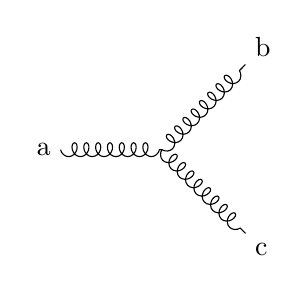
\begin{tikzpicture}
      \begin{feynman}
        \vertex (a) {a};
        \vertex [right=of a] (b);
        \vertex[above right= of b] (c) {b};
        \vertex[below right= of b] (d) {c};
        \diagram* {
          (a) -- [gluon] (b),
          (b) -- [gluon] (c),
          (b) -- [gluon] (d),
        };
      \end{feynman}
    \end{tikzpicture} \qquad
    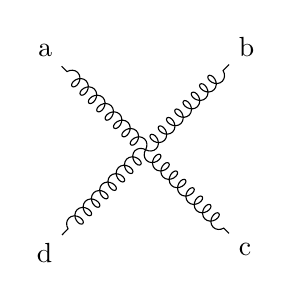
\begin{tikzpicture}
      \begin{feynman}
        \vertex (a);
        \vertex[above left=of a] (b) {a};
        \vertex[above right= of a] (c) {b};
        \vertex[below right= of a] (d) {c};
        \vertex[below left= of a] (e) {d};
        \diagram* {
          (a) -- [gluon] (b),
          (a) -- [gluon] (c),
          (a) -- [gluon] (d),
          (a) -- [gluon] (e),
        };
      \end{feynman}
    \end{tikzpicture}
    \caption{Feynman diagrams for gluons self-interactions}
    \label{fig:Feynman-gluons}
\end{figure}

The second term of Eq.~\ref{eq:Lqcd} describes the interactions between quarks and gluons, sketched in Fig.~\ref{fig:Feynman_q_g}, and contains the mass term for the fermions. It is noteworthy to observe that the interaction between quarks and gluons is diagonal in flavor, meaning that the strong interaction conserves the flavor of quarks. In contrast, colour mixing is allowed within the framework of QCD.

\begin{figure}[htb]
    \centering
    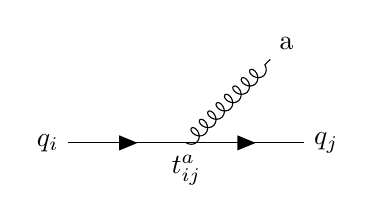
\begin{tikzpicture}
      \begin{feynman}
        \vertex (a);
        \vertex [below=0.1em of a] {$t^a_{ij}$};
        \vertex[left=of a] (b) {$q_i$};
        \vertex[right= of a] (c) {$q_j$};
        \vertex[above right= of a] (d) {a};
        \diagram* {
          (b) -- [fermion] (a),
          (a) -- [fermion] (c),
          (a) -- [gluon] (d),
        };
      \end{feynman}
    \end{tikzpicture}
    \caption{Feynman diagram for quark-gluon interaction}
    \label{fig:Feynman_q_g}
\end{figure}

\subsection{Running coupling constant}
If one considers a dimensionless physical observable, denoted in the following as $R$, which solely depends on a single energy scale, $Q$, one might naturally expect that $R$ would maintain a constant value, independent of the specific energy scale chosen. However, this does not hold true when loop diagrams are studied: the necessity of renormalisation introduces a new energy scale denoted as $\mu$. This scale, known as the renormalisation scale, is the point at which the subtraction of the ultraviolet divergences is carried out. Critically, $\mu$ is an arbitrary parameter and, as such, is non-physical. Consequently, $R$ becomes dependent on the ratio $Q^2/\mu^2$ and the renormalised coupling $\alpha_s = g_s^2/4\pi$: $R = R\left(\frac{Q^2}{\mu^2},\als\right)$. The $\mu$ independence of $R$ (which is an essential requirement given $\mu$'s arbitrariness) can be expressed as:
\begin{equation}\label{eq:RGE}
    \mu^2 \frac{\de R\left(\frac{Q^2}{\mu^2},\alpha_s\right)}{\de \mu^2} = \mu^2 \left[\frac{\partial}{\partial\mu^2}+\frac{\partial \alpha_s}{\partial\mu^2}\frac{\partial}{\partial\alpha_s}\right]R\left(\frac{Q^2}{\mu^2},\alpha_s\right) = 0\ , 
\end{equation}
a fundamental equation known as the renormalisation group equation. This equation is exactly true in the case of a prediction that considers all perturbative orders. If one limits the expansion at a fixed order $\alpha_s^N$, then a dependence of $R$ from $\mu$ is observed at the $\als^{N+1}$ order.\\ Solving Eq.~\ref{eq:RGE} requires the introduction of the concept of the running coupling $\alpha_s(Q^2)$, which evolves as a function of $Q$. By introducing
\begin{equation*}
    t\equiv \mathrm{log}(Q^2/\mu^2), \qquad \beta(\als)\equiv \mu^2 \frac{\de\als}{\mathrm{\mu^2}}\quad ,
\end{equation*}
Eq.~\ref{eq:RGE} can be written as
\begin{equation*}
    \left(-\frac{\partial}{\partial t} + \beta(\als)\frac{\partial}{\partial \als}\right) R(e^t,\als) = 0
\end{equation*}
This first-order partial differential equation can be solved by defining a new function: the running coupling $\als(Q^2)$
\begin{equation}\label{eq:t_integral}
    t = \mathrm{log}(Q^2/\mu^2) \equiv \int_{\als}^{\als(Q^2)} \frac{\de x}{\beta(x)} , \quad \mathrm{with}~\als=\als(\mu^2)\quad .
\end{equation}
By differentiating Eq.~\ref{eq:t_integral} with respect to $t$ and \als, one gets:
\begin{equation}\label{eq:beta_def}
    \beta(\als(Q^2)) = \frac{\partial\als(Q^2)}{\partial t}, \quad \frac{\de\als(Q^2)}{\de\als} = \frac{\beta(\als (Q^2))}{\beta(\als)}\quad .
\end{equation}
It results from this last set of equations that $R(1,\als(Q^2))$ satisfies Eq.~\ref{eq:RGE}; hence, the running coupling constant has absorbed the $\mu$ scale dependence of $R$. As a consequence, the knowledge of $R(1,\als)$, which can be evaluated in fixed-order perturbation theory, allows to know the dependence of $R$ from $Q^2$, which is the physical scale at which the coupling is gauged, by simply substituting $\als \rightarrow \als(Q^2)$. 

\subsubsection{The \ensuremath{\beta} function}
The running of the coupling constant is determined by the $\beta(\als)$ function, which is evaluated from loop corrections to the bare vertices of the theory. As of the time of the writing of this Thesis, the $\beta$ function has been evaluated up to 5 loops\cite{Herzog:2017ohr}. In Fig.~\ref{fig:beta_loops}, the 1-loop Feynman diagrams contributing to the $\beta$ function evaluation are reported.

\begin{figure}[htb]
    \centering
    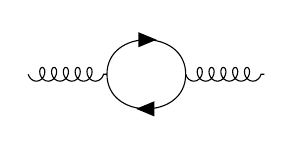
\begin{tikzpicture}
      \begin{feynman}
        \vertex (a);
        \vertex [right=1cm of a] (b);
        \vertex[right=1cm of b] (c);
        \vertex[right=1cm of c] (d);
        \diagram* {
            (a) -- [gluon] (b)
            -- [fermion, half left, looseness=1.5] (c)
            -- [fermion, half left, looseness=1.5] (b),
            (c) -- [gluon] (d),
        };
      \end{feynman}
    \end{tikzpicture}\quad
    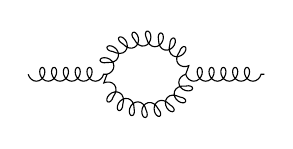
\begin{tikzpicture}
      \begin{feynman}
        \vertex (a);
        \vertex [right=1cm of a] (b);
        \vertex[right=1cm of b] (c);
        \vertex[right=1cm of c] (d);
        \diagram* {
            (a) -- [gluon] (b)
            -- [gluon, half left, looseness=1.5] (c)
            -- [gluon, half left, looseness=1.5] (b),
            (c) -- [gluon] (d),
        };
      \end{feynman}
    \end{tikzpicture}\quad
    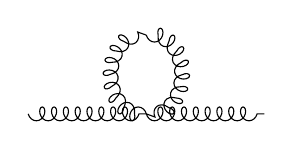
\begin{tikzpicture}
      \begin{feynman}
        \vertex (a);
        \vertex [right=of a] (b);
        \vertex[above=1cm of b] (c);
        \vertex[right=of b] (d);
        \diagram* {
            (a) -- [gluon] (b)
            -- [gluon, half left, looseness=1.5] (c)
            -- [gluon, half left, looseness=1.5] (b),
            (b) -- [gluon] (d),
        };
      \end{feynman}
    \end{tikzpicture}\quad

    \vspace{0.6cm}
    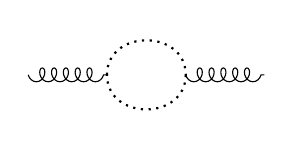
\begin{tikzpicture}
      \begin{feynman}
        \vertex (a);
        \vertex [right=1cm of a] (b);
        \vertex[right=1cm of b] (c);
        \vertex[right=1cm of c] (d);
        \diagram* {
            (a) -- [gluon] (b)
            -- [ghost, half left, looseness=1.5] (c)
            -- [ghost, half left, looseness=1.5] (b),
            (c) -- [gluon] (d),
        };
      \end{feynman}
    \end{tikzpicture}\quad
    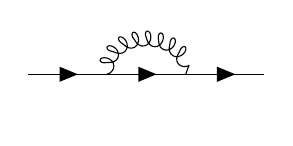
\begin{tikzpicture}
      \begin{feynman}
        \vertex (a);
        \vertex [right=1cm of a] (b);
        \vertex[right=1cm of b] (c);
        \vertex[right=1cm of c] (d);
        \vertex[below=0.31cm of c] (f) {$ $};
        \diagram* {
            (a) -- [fermion] (b) -- [fermion] (c) -- [fermion] (d),
            (b) -- [gluon, half left, looseness=1.5] (c)
            
        };
      \end{feynman}
    \end{tikzpicture}\quad
    
    \vspace{0.5cm}
    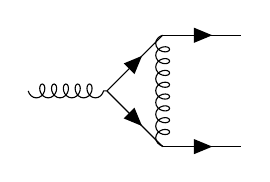
\begin{tikzpicture}
      \begin{feynman}
        \vertex (a);
        \vertex [right=1cm of a] (b);
        \vertex[above right=1cm of b] (c);
        \vertex[right=1cm of c] (d);
        \vertex[below right=1cm of b] (e);
        \vertex[right=1cm of e] (f);
        \diagram* {
            (a) -- [gluon] (b) -- [fermion] (c) -- [fermion] (d),
            (b) -- [fermion] (e) -- [fermion] (f),
            (c) -- [gluon] (e)
        };
      \end{feynman}
    \end{tikzpicture}\quad
    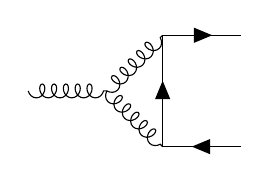
\begin{tikzpicture}
      \begin{feynman}
        \vertex (a);
        \vertex [right=1cm of a] (b);
        \vertex[above right=1cm of b] (c);
        \vertex[right=1cm of c] (d);
        \vertex[below right=1cm of b] (e);
        \vertex[right=1cm of e] (f);
        \diagram* {
            (a) -- [gluon] (b) -- [gluon] (c),
            (b) -- [gluon] (e),
            (f) -- [fermion] (e) -- [fermion] (c) -- [fermion] (d)
        };
      \end{feynman}
    \end{tikzpicture}\quad
    \caption{1-loop Feynman diagrams contributing to the $\beta$ function evaluation}
    \label{fig:beta_loops}
\end{figure}

By limiting the calculations at the first order in the perturbative expansion, one gets:
\begin{equation}\label{eq:beta0}
    \beta(\als) = -\als^2 \frac{11 \mathrm{N_c} - 2 \mathrm{N_f}}{12\pi} + \mathcal{O}(\als^3) \equiv -\als^2 \beta_0 + \mathcal{O}(\als^3)\quad ,
\end{equation}
where $\mathrm{N_c}$ is the number of colours (3), while $\mathrm{N_f}$ is the number of quark flavours which can be considered massless at the physical scale $Q^2$ at which the coupling is being measured.
From Eqs.~\ref{eq:beta0} and \ref{eq:beta_def}, one can extract the $Q^2$ dependency of the running coupling constant:
\begin{equation}\label{eq:alpha_s_running}
    \alpha_s(Q^2) = \frac{\alpha_s(\mu^2)}{1+\alpha_s(\mu^2)\beta_0 \mathrm{log}(Q^2/\mu^2)}\ ,
\end{equation}
Notably, since $\beta_0$ is positive also when considering 6 quark flavours, the strong coupling constant exhibits a monotonic decreasing trend as a function of $Q^2$. This behaviour differs from the one of the electromagnetic coupling constant, which increases with the energy scale due to the screening effect of vacuum polarisation. For QCD, the running of the coupling constant is a direct consequence of the non-Abelian nature of the theory, allowing for gluon self-interactions, which give rise to an anti-screening effect. The idea is that the emission of virtual gluons by static colour sources causes their colour charges to 'leak out' into the surrounding vacuum. Since the interaction between distributions of charges is weaker than the one between point-like charges when the distributions overlap, the effective coupling constant decreases at short distances. This behaviour is known as asymptotic freedom, a key feature of QCD that allows for the perturbative expansion of the theory at high energy scales, where the strong coupling constant is small. At the same time, the running of the coupling constant implies that the theory is non-perturbative at low energy scales, and phenomenological models are required to describe the strong interaction in this regime. Instead of using the renormalisation scale $\mu$ as a free parameter, one can use the running coupling constant to define a physical scale, $\Lambda_{QCD}$, which is the energy scale at which the coupling constant would diverge, if extrapolated outside the perturbative regime. Using Eq.~\ref{eq:alpha_s_running}, one can write:
\begin{equation*}
    \alpha_s(\Lambda_{QCD}) = \frac{1}{\beta_0 \mathrm{log}(Q^2/\Lambda_{QCD}^2)}\quad .
\end{equation*}
The value of $\Lambda_{QCD}$ is determined by its specific definition. However, to obtain the value of the coupling constant measured at $Q^2 = M_Z^2$, an approximate value of $\Lambda_{QCD}$ is around 200 MeV.

Measurements of the running of the coupling constant at different values of $Q$ are illustrated in Fig.~\ref{fig:alpha_s_running} and compared to the theoretical prediction at 5 loops. The agreement between the experimental data and the theoretical prediction is remarkable, confirming the validity of the QCD framework at high energy scales.


\begin{figure}[htb]
    \centering
    \includegraphics[width=0.7\linewidth]{Figures/Chapter 1/Alpha_s_running.png}
    \caption{Summary of measurements of \als as a function of the energy scale $Q$, compared to the running of the coupling computed at five loops, taking as an input the current PDG average, $\als(M_Z^2) = 0.1180 \pm 0.0009$ \gevcc.}
    \label{fig:alpha_s_running}
\end{figure}

\section{(De-)confinement}
The concept of confinement is one of the most intriguing aspects of QCD. It is the phenomenon by which quarks and gluons are never observed as free particles, but are always confined within colour-neutral hadrons. The confinement of quarks and gluons is a direct consequence of the non-Abelian nature of the theory, which, as described in the previous Section, is characterised by an increase of the strong coupling constant at low energy scales. This leads to the formation of colour-neutral hadrons, which are the only particles that can be observed in nature. The confinement of quarks and gluons is a non-perturbative effect, and the theoretical description of this phenomenon is still an open question in QCD. Some phenomenological models, such as the MIT bag model, have been proposed to describe confinement, but a complete understanding of this phenomenon is still lacking. Lattice QCD simulations are the most successful approach to study the non-perturbative regime of the theory, and they have provided a wealth of information on the properties of hadrons and the strong interaction at low energy scales.

\subsection{MIT bag model}
The MIT bag model~\cite{Johnson:1975zp} is a phenomenological model of confinement, which describes hadrons as bound states of quarks and gluons confined within a finite volume, called the bag. The model was developed in the 1970s by A. Chodos, R. L. Jaffe, K. Johnson, C. B. Thorn, and V. F. Weisskopf, and it has been widely used to study the properties of hadrons and the strong interaction. In the MIT bag model, N masslesss fermions are confined within a spherical cavity of radius $R$, which is the bag radius. The confinement arises from a balance between pressure due to the kinematic energy of the fermions inside the bag and an ad hoc external pressure, which is introduced to confine the fermions within the bag. The fermions are described by the Dirac equation for massless fermions:

\begin{equation*}
    i\gamma^\mu\partial_\mu\psi = 0\quad ,
\end{equation*}
where $\psi$ is the fermion field, and $\gamma^\mu$ are the Dirac matrices. The solution to the Dirac equation is given in terms of the spherical Bessel functions of the zeroth and first order, $j_0(p_0r)$ and $j_1(p_0r)$, where $p_0$ is the energy of the fermion:

\begin{equation*}
    \psi = \mathcal{N} e^{-ip_0t} \begin{pmatrix} j_0(p_0r)\chi^+ \\ \vec{\sigma}\cdot\hat{r}j_1(p_0r)\chi^-\end{pmatrix}\quad ,
\end{equation*}
where $\chi^+$ and $\chi^-$ are the two components of the fermion four dimentional spinor $\psi$, and $\vec{\sigma}$ are the Pauli matrices. The colour flux at a point $r$ inside the bag is given by:

\begin{equation*}
    j_{ab}^\mu(r) = \bar{\psi_a}(r)\gamma^\mu\psi_b(r)\quad ,
\end{equation*}
where $a$ and $b$ are the colour indices of the fermions. If the quantum numbers are not to be lost through the surface of the bag, which is the definition of confinement, then:

\begin{equation*}
  n_\mu j_{ab}^\mu(r) = \bar{\psi_a}(r)\gamma\cdot n \psi_b(r) = 0\quad ,
\end{equation*}
on the surface, where $n$ is a unit space-like vector normal to the surface. Using the gamma properties, $(i\gamma\cdot n)^2 = 1$, so that by assuming that $i\gamma\cdot n = + 1$, the boundary condition on the surface of the bag is given by:

\begin{equation*}
    \bar{\psi}(R)\psi(R) = 0\quad ,
\end{equation*}
leading to the solution of the Dirac equation in the bag:

\begin{equation*}
    \left[j_0\left(p_0R\right)\right]^2 - \left[j_1\left(p_0R\right)\right]^2 = 0\quad ,
\end{equation*}
with solution $p_0R = 2.04$. The total energy inside the bag is given by:

\begin{equation*}
    E = \frac{2.04 N}{R}(\hbar c) + \frac{4\pi}{3}R^3B\quad ,
\end{equation*}
where the first term is the kinetic energy of the fermions, and the second term is the energy due to the presence of an external pressure $B$ which keeps the fermions confined in the bag. The bag pressure is a phenomenological parameter of the model, and it is introduced to confine the fermions within the bag. It can be extracted by minimising the energy of the system with respect to the bag radius $R$, yielding $B=234$ MeV/fm$^3$, for a baryon with $R=0.8$ fm.

\subsection{Deconfinement}
The concept of deconfinement refers to the transition from a confined state to a state where quarks and gluons are no longer confined within hadrons, but are free to move in a larger volume. As modelled by the MIT bag model, non-perturbative QCD effects can be described in terms of an external pressure, which confines quarks and gluons within a finite volume. If the external pressure is overcome by the pressure due to the kinematic energy of the quarks and gluons, then the hadrons constituents are no longer confined, and a transition to a state called Quark-Gluon Plasma (QGP) occurs. The QGP is characterised by extremely high temperatures and energy densities, and it is believed to have existed in the early universe, a few microseconds after the Big Bang. The internal pressure of the bag can increase in two different regimes: by increasing the temperature of the system (hot QGP), or by increasing the baryonic density (cold QGP). For the former, temperatures of about 155 MeV are required to overcome the bag pressure, while for the latter, baryonic densities of about 5 times those of nuclei are needed. The QGP is a unique state of matter that can be studied in the laboratory by colliding heavy ions at high energies. In these collisions, a hot and dense medium is created, where quarks and gluons are no longer confined within hadrons, but are free to move in a larger volume. The study of the QGP is an active area of research in nuclear and particle physics, and it provides valuable insights into the properties of the strong interaction at high energy scales.
Direct observation of the primordial QGP (i.e. that created just after the Big Bang) would provide a wealth of information on the early universe; however, the universe underwent a phase in which electrons were not bound to nuclei, making the universe opaque to electromagnetic radiation, and denying us the possibility of directly observing the QGP. Once the universe cooled enough (3000 K) to allow electrons to bind to nuclei, the electromagnetic radiation decoupled with a black body spectrum of around 3000 K. Since then, as the universe expanded, this electromagnetic radiation has redshifted to a temperature of around 2.7 K, and is denoted as the Cosmic Microwave Background (CBM). The CMB is the oldest light in the universe and provides a snapshot of the universe when it was 300,000 years old, way after the QGP had already cooled down. Hence, the only way to study the QGP is by recreating it in the laboratory, by colliding heavy ions at high energies. In the past decades, several experiments~\cite{ALICE:2022wpn, NA38:2000wlp, NA50:1997hlx, Nouicer:2009fy} have been carried out to study the properties of this state of matter, and the results have provided valuable insights into the properties of the strong interaction at high energy scales.

\subsection{Lattice QCD}
Lattice QCD is a numerical technique used to study the non-perturbative regime of QCD. The method is based on the discretisation of spacetime on a four-dimensional lattice, and the evaluation of the path integral of the theory by Monte Carlo methods, i.e. by sampling possible configurations of the quark and gluon fields according to the probability distribution given by the QCD Lagrangian. The lattice spacing is a parameter of the method, and allows one to avoid the ultraviolet divergences of the theory, which are typical in perturbative QCD, by introducing a cutoff on the momenta of the quark and gluon fields. 
\begin{figure}[htb]
  \centering
  \includegraphics[width=0.7\linewidth]{Figures/Chapter 1/PathIntegrals.png}
  \caption{Feynman introduction to path integrals. Here, a particle emitted from a source at $x_a$ is detected at $x_b$. A finite number of screens, each with a finite number of holes, is placed between the source and the detector. The probability amplitude for the particle to hit the detector is given by the sum of the probabilities of moving from the source to the detector through all possible paths. By adding an infinite amount of screens with an infinite number of holes, and by also considering the time at which the particle passes through the screens, the sum becomes an integral over all possible paths, called a \emph{path integral}.}
  \label{fig:PathIntegrals}
\end{figure}
The Lattice QCD simulations are based on the path integral formalism of quantum field theory~\cite{RevModPhys.20.367}, developed by R. Feynman in the 1940s. The path integral provides a natural extension of the least action principle of classical mechanics to quantum mechanics, and it allows one to calculate the probability amplitude of a particle to move from one point to another in spacetime, considering the evolution of the system over all possible paths. The transition amplitude from the state $(x_a,t_a)$ to the state $(x_b,t_b)$ is given by:
\begin{equation}\label{eq:ampl_prob}
  A \left[(x_a,t_a) \rightarrow (x_b,t_b) \right] = \braket{x_b,t_b | e^{-iH(t_b-t_a)} | x_a,t_a} = \sum_\mathrm{paths} e^{iS[x(t)]}\quad , 
\end{equation}
where $H$ is the Hamiltonian of the system, $S[x(t)]$ is the action of the system, and the sum is over all possible paths from $(x_a,t_a)$ to $(x_b,t_b)$. By taking the continuum limit on space-time, we obtain an integration over all the possible space-time paths of the system:
\begin{equation}\label{eq:path_integral}
  \sum_\mathrm{paths} e^{iS[x(t)]} \rightarrow \int_{x_a}^{x_b} \left[\mathcal{D}x(t)\right] e^{iS[x(t)]}\quad ,
\end{equation}
where the right-hand side term is a functional integral over all possible paths of the system. It is interesting to note that by combining Eqs.~\ref{eq:ampl_prob} and \ref{eq:path_integral}, one gets a quantity resembling the partition function of a statistical system:
\begin{equation*}
  \mathcal{Z} = \sum_{x_a} \braket{x_a,t_a | e^{\beta H} | x_a,t_a}\quad .
\end{equation*}
It is possible to express the partition function in terms of a path integral by applying a Wick rotation to the time variable, $t \rightarrow -i\tau$, with $\tau_a=0\leq\tau\leq\tau_b=\beta$ and considering the Euclidean action in place of the Minkowskian one, $S_E = iS$. Furthermore, since the state at $\tau_a$ is the same as the one at $\tau_b$, a periodic boundary condition is imposed: $x(\tau_a) = x(\tau_b)$. With these considerations, the partition function can be expressed as:
\begin{equation*}
  \mathcal{Z} = \int \left[\mathcal{D}x(\tau)\right] e^{-S_E[x(\tau)]}\quad .
\end{equation*}
This formalism, which was here developed for a single particle, can be extended to a quantum field theory, and in particular to QCD.

The lattice QCD simulations are computationally intensive, and they require large supercomputers to perform the calculations. To limit the computational costs, calculations are often performed at larger up and down quark masses than in nature, drastically reducing the number of virtual quark-antiquark loops that have to be taken into account. Because of the employed Monte Carlo approach, only a finite number of configurations can be considered, leading to statistical uncertainties in the lattice QCD results. In order to obtain physical results, several limits have to be taken: i. the continuum limit, i.e. the extrapolation of the lattice spacing to zero, ii. the infinite-volume limit, i.e. the extrapolation of the lattice size to infinity, and iii. the physical quark-mass limit, i.e. the extrapolation to physical quark masses, although many present-day lattice calculations are already performed directly at, or very close to, the physical values of the quark masses, so that the latter extrapolation becomes less of an issue. 

The results of the lattice QCD simulations are in good agreement with the experimental data, and they have provided valuable insights into the properties of the strong interaction at low energy scales. For example, Fig.~\ref{fig:LQCD_hadron_mass} shows the spectrum of hadrons obtained from lattice QCD simulations, taken from~\cite{BMW:2008jgk}, compared to the experimental data. The agreement between the lattice QCD results and the experimental data is remarkable, confirming the validity of the QCD framework at low energy scales.
\begin{figure}
  \centering
  \includegraphics[width=0.7\linewidth]{Figures/Chapter 1/LQCD_hadron_mass.png}
  \caption{The light hadron spectrum of QCD. Horizontal lines and bands are the experimental values with their decay widths. Lattice QCD results~\cite{BMW:2008jgk} are shown by solid circles. Vertical error bars represent the combined statistical and systematic error estimates. $\pi$, K and $\Xi$ have no error bars, because they are used to set the light quark mass, the strange quark mass and the overall scale, respectively.}
  \label{fig:LQCD_hadron_mass}
\end{figure}
\setcounter{chapter}{1}
%\chapter{Open heavy-flavour production in proton-proton collisions}\label{ch:openHF}

Open heavy-flavour hadrons, composed of a heavy quark (charm or beauty) along with lighter quarks, are exclusively formed in high-momentum transfer processes due to the large masses of approximately 1.3 \gevcc and 4.2 \gevcc~\cite{pdg} for charm and beauty quarks, respectively. As a result, heavy quarks are created in the early stages of the collision, and their production cross-section in the partonic interaction can be evaluated perturbatively using QCD. Studying the production of open heavy-flavour hadrons in proton-proton (pp) collisions not only provides a crucial test of the perturbative QCD framework, but also allows to set constraints on heavy-quark hadronisation models. Furthermore, measurements in proton-proton collisions, where the production of an extended deconfined medium is not expected, are a necessary reference for the study of heavy-ion collisions, where the properties of the QGP can be investigated. 

\section{Factorisation theorem}
The production of open heavy-flavour hadrons in proton-proton collisions can be described using the factorisation theorem~\cite{Collins:1989gx}, which allows for the separation of short-distance, perturbative behaviour from long-distance, non-perturbative phenomena. The total production cross-section can be expressed as
\begin{equation}\label{eq:pp_xsec}
    \sigma_{\text{pp}}^\mathrm{H} = \sum_\mathrm{a,b = g, q, \overline{q}} \int \de x_1 \de x_2 f_\mathrm{a/A}(x_1,\mu_\mathrm{F}^2) f_\mathrm{b/B}(x_2,\mu_\mathrm{F}^2) \hat{\sigma}_\mathrm{ab \rightarrow Q\overline{Q}} (x_1,x_2,\mu_\mathrm{F}^2,\mu_\mathrm{R}^2) D_\mathrm{Q\rightarrow H_Q}(z,\mu_\mathrm{F}^2) \quad ,
\end{equation}
i.e., the convolution of: i) the Parton Distribution Functions (PDFs) $f_\mathrm{a/A}(x_1,\mu_\mathrm{F}^2)$ and $f_\mathrm{b/B}(x_2,\mu_\mathrm{F}^2)$, describing the initial-state probability of finding a parton a in the proton A carrying a fraction $x_1$ of the proton's momentum, and a parton b in the proton B carrying a fraction $x_2$ of its momentum, respectively; ii) the hard partonic scattering cross-section $\hat{\sigma}_\mathrm{ab \rightarrow Q\overline{Q}} (x_1,x_2,\mu_\mathrm{F}^2,\mu_\mathrm{R}^2)$, defining the probability of producing the $\mathrm{Q\overline{Q}}$ final state from the collision of partons a and b, where Q is either a charm or beauty quark; and iii) the Fragmentation Functions (FFs) $D_\mathrm{Q\rightarrow H_Q}(z,\mu_\mathrm{F}^2)$, which describe the probability of the heavy quark Q to fragment into a heavy-flavour hadron $\mathrm{H_Q}$ carrying a fraction of the parent parton momentum $z$. $\mu_\mathrm{F}$ and $\mu_\mathrm{R}$ are the factorisation and renormalisation scales, respectively. The former is the scale at which the non-perturbative processes are separated from the perturbative ones, while the latter is the scale at which the ultraviolet divergences, emerging from the calculations of scattering amplitudes involving loop diagrams, are subtracted. While the PDFs and FFs are non-perturbative quantities, parametrised from experimental data and regarded as universal across different collision systems, the hard partonic scattering cross-section can be perturbatively calculated using QCD, but needs specific evaluations for each process. 

The factorisation theorem has been widely employed to describe the production of open heavy-flavour hadrons in proton-proton collisions, and has proven to be successful in modeling experimental data. Figure~\ref{fig:ppDmeson} shows the production cross-section of prompt and non-prompt $\mathrm{D^0}$-mesons in proton-proton collisions at $\sqrt{s} = 5.02$~\tev measured at midrapidity ($\lvert y\rvert<0.5$) as a function of the transverse momentum (\pt) by the ALICE Collaboration~\cite{ALICE:2021mgk}, compared to Fixed-Order plus Next-to-Leading Logarithms (FONLL) perturbative QCD predictions~\cite{Cacciari:1998it} combined with the \textsc{Pythia}~8~\cite{Sjostrand:2014zea} event generator for the $\mathrm{H_b \rightarrow D^0+X}$ decay kinematics. The calculation is performed at next-to-leading order, including all the $\als^2$ and $\als^3$ terms, with the resummation of the next-to-leading logarithmic terms. These include terms of the form $\alpha_s^2\alpha_s^k\log^k(\pt/m)$ and $\alpha_s^3\alpha_s^k\log^k(\pt/m)$, where $m$ is the heavy-quark mass. The term \emph{prompt} refers to charm-hadrons directly produced in the hadronisation of a charm quark or through the strong decay of a directly produced excited charm-hadron or charmonium state, while \emph{non-prompt} charm hadrons are produced in the decay of a hadron containing a beauty quark. The FONLL predictions are in good agreement with the non-prompt $\mathrm{D^0}$-meson production cross-section, whereas the prompt contribution lies at the upper edge of the theoretical uncertainty band, albeit being described within the uncertainties. Similar trends are observed in the production of other open heavy-flavour hadrons across different experimental facilities, such as the Tevatron~\cite{CDF:2003vmf}, RHIC~\cite{STAR:2012nbd}, and LHC~\cite{ALICE:2021mgk}.

\begin{figure}[htb]
    \centering
    \includegraphics[width=0.6\linewidth]{Figures/Chapter 2/CrossSectionD0_Prompt_NonPrompt_pp5TeV_vsFONLL_Pythia8_BRnative_1.pdf}
    \caption{\pt-differential production cross-section of prompt and non-prompt $\mathrm{D^0}$-mesons measured at midrapidity ($\lvert y\rvert<0.5$) in pp collisions by the ALICE Collaboration at $\sqs=5.02$~\tev~\cite{ALICE:2021mgk} compared to predictions obtained with FONLL calculations~\cite{Cacciari:1998it} combined with \textsc{Pythia}~8~\cite{Sjostrand:2014zea} for the $\mathrm{H_b \rightarrow D^0+X}$ decay kinematics. Figure taken from Ref.~\cite{ALICE:2021mgk}}
    \label{fig:ppDmeson}
\end{figure}

\subsection{Parton Distribution Functions}
\subsubsection{Deep inelastic scattering}
The PDFs are non-perturbative quantities describing the probability of finding a parton carrying a fraction $x$ of the proton's momentum in the initial state of a process. The first experimental evidence revealing the partonic structure of the proton emerged from deep inelastic scattering experiments carried out at the Stanford Linear Accelerator Center (SLAC) in the 1960s~\cite{Friedman:1972sy}, where an electron was scattered off a proton with momentum $P$
, and the transferred momentum $q$ was measured. The cross-section for deep inelastic scattering can be defined in terms of the Lorentz invariant variables $Q^2 = -q^2$ and $x = \frac{Q^2}{2P\cdot q}$, yielding
\begin{equation*}
    \frac{\de^2\sigma}{\de x \de Q^2} = \frac{4\pi\alpha^2}{xQ^4} \left[ \left(1-y\right)F_2(x,Q^2) - xy^2F_1(x,Q^2) \right]\quad ,
\end{equation*}
where $y=Q^2/(sx)$, $s = (P+p_\mathrm{e})^2$ denotes the centre-of-mass energy of the electron-proton system, and the structure functions $F_1(x,Q^2)$ and $F_2(x,Q^2)$ represent an extension of the form factors for elastic scattering.
The first measurements of high-energy inclusive inelastic scattering experiments were performed using a 20~GeV linear accelerator at SLAC, and showed that the structure functions $F_1(x,Q^2)$ and $F_2(x,Q^2)$ were independent of $Q^2$ at fixed $x$ within the studied $1<~Q^2~<~10$~\gevcc range. This was in contrast with the behavior observed for the proton elastic form factors, where a decrease of two orders of magnitude was observed within the same $Q^2$ interval. This independence of the structure functions from $Q^2$ in deep inelastic scatterings was predicted by Bjorken in 1968 for $Q^2 \rightarrow \infty$~\cite{Bjorken:1968dy}, and is known as \emph{Bjorken scaling}. A physical interpretation of this phenomenon arrived just one year later, in 1969, with Feynman's parton model~\cite{Feynman:1969ej}, which described the interaction in terms of elastic scattering of the probe off a point-like constituent (parton) within the proton. This model explains the scale-invariance property of the proton structure functions, as the scattering centres are assumed to be structure-less. In this picture, the Bjorken variable $x$ acquires a new interpretation as the fraction of the proton momentum carried by the struck parton. The parton model also offers a straightforward definition of the structure functions in terms of the parton distribution functions $f_\mathrm{a}(x)$:
\begin{equation*}
    F_2(x,Q^2) = \sum_\mathrm{a} e_\mathrm{a}^2 x f_\mathrm{a}(x)\quad ,
\end{equation*}
where the sum is over partons with electric charge $e_\mathrm{a}$, and $f_\mathrm{a}$ are unknown, but universal functions for a given hadron, describing the probability of finding a parton of type a with a fraction $x$ of the proton's momentum. 

To explore the spin properties of the partons, the structure functions $F_1$ and $F_2$ were studied at different centre-of-mass energies. By investigating the relationship between the two structure functions, it was established that the partons have spin 1/2, as the Callan-Gross relation~\cite{Callan:1969uq}, which holds true for point-like Dirac particles, was found to be satisfied:
\begin{equation*}
    F_2(x,Q^2) = 2x F_1(x,Q^2)\quad .
\end{equation*}

In the next years, it became clear that additional constituents within the proton carry momentum but lack electric or weak charge, as the so-called momentum sum rule was not saturated by the measured PDFs in electron and neutrino scatterings. This missing momentum was attributed to gluons, which were discovered in the 1970s and are the field quanta of the strong force.

\subsubsection{Bjorken scaling violation}
\begin{figure}[htb]
    \centering
    \includegraphics[width=0.6\linewidth]{Figures/Chapter 2/F2Results.png}
    \caption{The proton structure function $F^p_2$ measured in electromagnetic scattering of electrons and positrons on protons, and for electrons/positrons and muons on a fixed target~\cite{pdg}.}
    \label{fig:scaling_violation}
\end{figure}
By the late 1970s, measurements of the structure functions at larger $Q^2$ values taken at CERN and DESY revealed that Bjorken scaling was violated, i.e., the structure functions were not $Q^2$ independent. Figure~\ref{fig:scaling_violation} shows measurements of the proton structure functions $F_2(x,Q^2)$ as a function of $Q^2$ for various values of $x$ taken from different experiments~\cite{pdg}. It is clear from the plot that structure functions present an increasing trend as a function of $Q^2$ at low $x$, and a decreasing trend as a function of $Q^2$ at high $x$. 

The parton model fails to explain this behaviour, as it relies on the assumption that the transferred energy is sufficiently large to neglect the proton and its constituents' masses, as well as the interactions among partons. In particular, the partons' transverse momentum with respect to the proton momentum is neglected. The key to understanding Bjorken scaling violation comes from QCD and the realisation that the parton's transverse momentum is not necessarily restricted to be small. A quark, for instance, can emit a gluon and acquire large transverse momentum $k_T$ with a probability proportional to $\als \de k_T/k_T^2$ at large $k_T$. The integral extends up to the kinematic limit $k_T\sim Q^2$, giving rise to contributions proportional to $\als\mathrm{log}Q^2$, which break the scaling. The evolution of PDFs with $Q^2$ from a parametrisation at a given $Q^2_0$ can be perturbatively described using the Dokshitzer-Gribov-Lipatov-Altarelli-Parisi (DGLAP) evolution equations~\cite{Gribov:1972ri,Dokshitzer:1977sg,Altarelli:1977zs}, which require the introduction of a new arbitrary scale, at which the factorisation of the non-perturbative processes happens: the factorisation scale $\mu_\mathrm{F}$. There exists a wide range of PDF parametrisations, such as the NNPDF~\cite{NNPDF:2021njg}, CTEQ~\cite{Dulat:2015mca}, and MMHT~\cite{Harland-Lang:2014zoa}, which are determined from global fits to a wide range of experimental data, including deep inelastic scattering, Drell-Yan, and jet production.
\subsection{Partonic cross-section}\label{sec:partonic_cross_section}
\begin{figure}[htb]
    \centering
    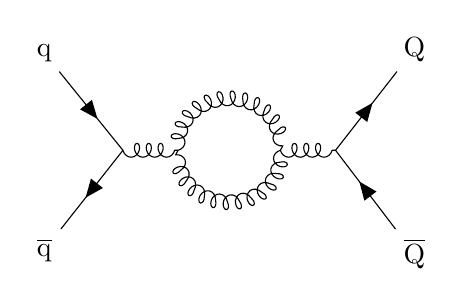
\begin{tikzpicture}
      \begin{feynman}
        \vertex (a);
        \vertex [above=1cm of a] (b) {q};
        \vertex[below=1cm of a] (c) {$\overline{\mathrm{q}}$};
        \vertex[right=1cm of a] (d);
        \vertex[right=0.7cm of d] (e);
        \vertex[right=1.3cm of e] (f);
        \vertex[right=0.7cm of f] (g);
        \vertex[right=1cm of g] (h);
        \vertex[above=1cm of h] (i) {Q};
        \vertex[below=1cm of h] (j) {$\overline{\mathrm{Q}}$};
        \diagram* {
            (b) -- [fermion] (d) -- [fermion] (c),
            (d) -- [gluon] (e),
            (e) -- [gluon,  in=90, out=90, looseness=1.7] (f) -- [gluon,  in=-90, out=-90, looseness=1.7] (e),
            (f) -- [gluon] (g),
            (j) -- [fermion] (g) -- [fermion] (i),
        };
      \end{feynman}
    \end{tikzpicture}\quad
    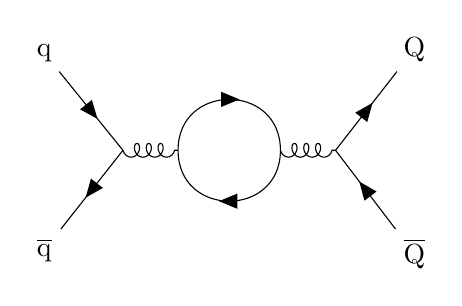
\begin{tikzpicture}
        \begin{feynman}
          \vertex (a);
          \vertex [above=1cm of a] (b) {q};
          \vertex[below=1cm of a] (c) {$\overline{\mathrm{q}}$};
          \vertex[right=1cm of a] (d);
          \vertex[right=0.7cm of d] (e);
          \vertex[right=1.3cm of e] (f);
          \vertex[right=0.7cm of f] (g);
          \vertex[right=1cm of g] (h);
          \vertex[above=1cm of h] (i) {Q};
          \vertex[below=1cm of h] (j) {$\overline{\mathrm{Q}}$};
          \diagram* {
              (b) -- [fermion] (d) -- [fermion] (c),
              (d) -- [gluon] (e),
              (e) -- [fermion,  in=90, out=90, looseness=1.7] (f) -- [fermion,  in=-90, out=-90, looseness=1.7] (e),
              (f) -- [gluon] (g),
              (j) -- [fermion] (g) -- [fermion] (i),
          };
        \end{feynman}
      \end{tikzpicture}

    \vspace*{0.5cm}
    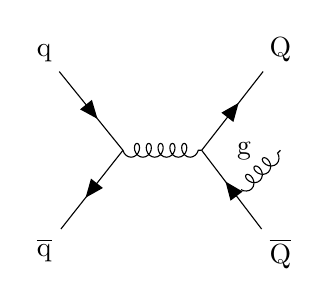
\begin{tikzpicture}
        \begin{feynman}
          \vertex (a);
          \vertex [above=1cm of a] (b) {q};
          \vertex[below=1cm of a] (c) {$\overline{\mathrm{q}}$};
          \vertex[right=1cm of a] (d);
          \vertex[right=1cm of d] (e);
          \vertex[right=1cm of e] (f);
          \vertex[above=1cm of f] (g) {Q};
          \vertex[below=1cm of f] (h) {$\overline{\mathrm{Q}}$};
          \vertex[right=0.5cm of e] (i);
          \vertex[below=0.5cm of i] (j);
          \diagram* {
              (b) -- [fermion] (d) -- [fermion] (c),
              (d) -- [gluon] (e),
              (h) -- [fermion] (e) -- [fermion] (g),
              (j) -- [gluon, edge label = g] (f),

          };
        \end{feynman}
      \end{tikzpicture}\quad
      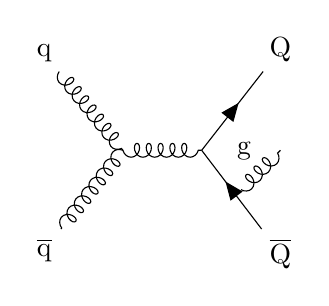
\begin{tikzpicture}
        \begin{feynman}
            \vertex (a);
            \vertex [above=1cm of a] (b) {q};
            \vertex[below=1cm of a] (c) {$\overline{\mathrm{q}}$};
            \vertex[right=1cm of a] (d);
            \vertex[right=1cm of d] (e);
            \vertex[right=1cm of e] (f) ;
            \vertex[above=1cm of f] (g) {Q};
            \vertex[below=1cm of f] (h) {$\overline{\mathrm{Q}}$};
            \vertex[right=0.5cm of e] (i);
            \vertex[below=0.5cm of i] (j);
          \diagram* {
              (b) -- [gluon] (d) -- [gluon] (c),
              (d) -- [gluon] (e),
              (h) -- [fermion] (e) -- [fermion] (g),
              (j) -- [gluon, edge label = g] (f),

          };
        \end{feynman}
      \end{tikzpicture}\quad
      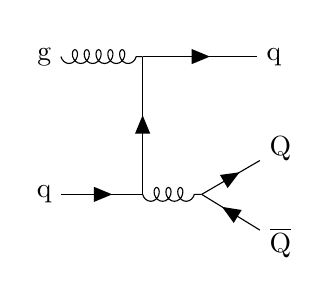
\begin{tikzpicture}
        \begin{feynman}
          \vertex (a) {g};
          \vertex[above=0.25cm of a] (spacing) {$ $  }; 
          \vertex[right=1.25cm of a] (b);
          \vertex[right=1.45cm of b] (c) {q};
          \vertex[below=1.75cm of a] (d) {q};
          \vertex[right=1.25cm of d] (e);
          \vertex[right=0.75cm of e] (f);
          \vertex[right=1cm of f] (g);
          \vertex[above=0.3cm of g] (h) {Q};
          \vertex[below=0.3cm of g] (j) {$\overline{\mathrm{Q}}$};
          \diagram* {
                (a) -- [gluon] (b),
                (d) -- [fermion] (e) -- [fermion] (b) -- [fermion] (c),
                (e) -- [gluon] (f),
                (j) -- [fermion] (f) -- [fermion] (h),
          };
        \end{feynman}
      \end{tikzpicture}\quad
    \caption{Feynman diagrams contributing to the first order corrections of the heavy-flavour production cross-section calculations.}
    \label{fig:NLO_diagrams}
\end{figure}

\begin{sloppypar}
Because of their large masses, heavy quarks can only be produced through hard-scattering processes, characterised by momentum transfers of the order of \mbox{$Q^2 \geq 4m^2_\mathrm{b,c}$}. In this regime, the strong coupling constant is significantly smaller than unity, allowing for the perturbative calculation of the heavy quark production cross-section from partonic scattering using QCD. While predictions at next-to-next-to-next-to-leading order (N$^3$LO) are available for certain processes, such as Higgs production~\cite{Anastasiou:2015vya, Anastasiou:2016cez}, the current state-of-the-art calculations for charm-quark production are at next-to-leading order (NLO) with all-order resummation to next-to-leading logarithmic (NLL) accuracy in the limit where the \pt of a heavy quark is much larger than its mass~\cite{Cacciari:1998it}. The contributions arising at the NLO include 1-loop virtual corrections to the Born process and real emission of a gluon or a quark-antiquark pair, and are depicted in Fig~\ref{fig:NLO_diagrams}. Next-to-next-to-leading order (NNLO) QCD radiative corrections to the production of bottom-quark pairs have also been computed~\cite{Catani:2020kkl}.
\end{sloppypar}

\subsection{Fragmentation Functions}
\begin{sloppypar}
Quarks and gluons produced in hard-scattering processes ultimately give rise to colourless observable hadrons. The associated process, known as hadronisation, is non-perturbative since the partonic processes involved are characterised by relatively small energy scales ($\sim\Lambda_\mathrm{QCD}$), where the strong coupling constant is large. The hadronisation process is described by the Fragmentation Functions (FFs) $D_\mathrm{Q\rightarrow H_Q}(z,\mu_\mathrm{F}^2)$, which parametrise the probability of the heavy quark Q to fragment into a heavy-flavour hadron $\mathrm{H_Q}$ with a fraction of the parent parton momentum $z$. They provide a simple ``effective" description of the parton-to-hadron transition by mapping the quark-momentum-differential cross-section into the hadron-momentum differential one. FFs are typically determined from experimental data, usually by analyzing the final-state hadrons produced in electron-positron collisions where the initial momenta are well-known. These FFs are then applied in the evaluation of cross-sections in other colliding systems, assuming that the relevant hadronisation processes are “universal”, i.e., independent of the collision energy and system. This assumption implies the hypothesis of \emph{independent fragmentation}, which states that the hadronisation of the parton produced in the hard-scattering process is independent of the production mechanism and the partonic environment which surrounds it. Differently from the fragmentation of light quarks and gluons, kinematic considerations on heavy-quark fragmentation~\cite{Bjorken:1977md,Suzuki:1977km} suggest that heavy hadrons tend to carry a larger fraction of the parent parton momentum. Fragmentation functions for heavy quarks are therefore shifted towards higher values of $z$ compared to those of light quarks and gluons~\cite{Peterson:1982ak}. Many FFs have been determined from global fits to data, such as the NNFF1.1h~\cite{Bertone:2018ecm}, DSS~\cite{deFlorian:2007aj}, and KKP~\cite{Kniehl:2000fe} parametrisations for light flavours, and typically differ in the data sets used for the fit, the treatment of the data, and the functional form of the FFs. Parametrisations for heavy quark fragmentation include that of Peterson et al.~\cite{Peterson:1982ak}, Kartvelishvili et al.~\cite{Kartvelishvili:1977pi}, and Breetan et al.~\cite{Braaten:1994bz}. Similarly to PDFs, FFs also evolve with the energy scale of the interaction, and this evolution is described perturbatively by the DGLAP equations. 
\end{sloppypar}

\section{Hadronisation: microscopic and macroscopic descriptions}\label{sec:hadronisation}
Despite being a very powerful effective tool for describing heavy-flavour hadron production, the parametrisation of fragmentation functions used in a factorisation-theorem approach is not the only method used to describe the hadronisation of energetic quarks in high-energy collisions. Over the years, other models have been developed to describe hadron production starting from a partonic stage (e.g., quarks and gluons from the initial hard-scattering process, and those being radiated from the initial partons) and implementing a colour neutralisation procedure that groups quarks and gluons into hadrons.

The standard approach for describing the complex event topologies in these models, which are typically implemented in Monte Carlo event generators, begins with a matrix-element calculation for the production of a few well-separated partons, followed by the application of a parton shower. The \emph{parton shower} provides an approximate perturbative treatment of QCD dynamics, which is then combined with a non-perturbative model for the hadronisation process at a certain infrared cut-off scale, typically taken to be of the order of 1~\gev. The basic idea of the parton shower relies on the Sudakov form factor~\cite{Sudakov:1954sw}, which expresses the probability of a parton not radiating another parton in a given phase space region. If a parton does radiate, the newly-produced parton becomes the source of a new cascade, continuing until the parton shower terminates at the hadronisation scale. At this point, partons are allowed to fragment into hadrons through hadronisation models. 

Although several hadronisation models have been developed, each implementing a different approach to the description of this non-perturbative process, a common feature is the hypothesis of local parton-hadron duality~\cite{Azimov:1984np}, which states that the flow of momentum and quantum numbers at the hadron level tends to follow the flow established at the parton level.

\subsection{Independent fragmentation}\label{sec:independent_fragmentation}
The description of the hadronisation process using FFs relies on the assumption of \emph{independent fragmentation}, i.e., the probability of a parton fragmenting into a hadron is considered independent of the other partons produced in the same collision, effectively considering the hadronisation process as universal, i.e., independent of the collision energy and system. In the original scheme proposed by R. Field and R. Feynman~\cite{Field:1976ve}, the fragmenting quark combines with an antiquark from a $\mathrm{q\overline{q}}$ pair produced from the vacuum to create a meson with energy fraction $z$. The remaining quark, with energy fraction $(1-z)$, fragments in the same way, continuing until an energy cut-off is reached. The probability distribution of $z$ is the fragmentation function. The assumption of independent fragmentation is valid in the case of low-multiplicity \ee collision events, where the number of produced partons is small and no hadronic remnants are present.

However, recent results on the production of strange and heavy-flavour baryons in proton-proton and proton-lead collisions at the LHC~\cite{ALICE:2020wla,ALICE:2024ozd} show that a description of the hadronisation process based on independent fragmentation is not sufficient to describe the data, as it significantly underestimates the baryon production. Figure~\ref{fig:Lambda_c_D0_ee} shows the $\mathrm{\lc/D^0}$ production-yield ratio measured at midrapidity ($\lvert y\rvert<0.5$) in pp collisions at $\sqrt{s} = 5.02$~\tev by the ALICE Collaboration~\cite{ALICE:2020wla} as a function of \pt, compared to theoretical predictions. The predictions are obtained from: i) \textsc{Pythia}~8 with Monash tune~\cite{Skands:2014pea}; ii) HERWIG~7~\cite{Bellm:2015jjp}; iii) POWHEG~\cite{Frixione:2007nw} NLO pQCD calculations, matched with \textsc{Pythia}~6 to generate the parton shower; iv) General-Mass Variable-Flavour-Number Scheme~\cite{Kniehl:2005mk} (GM-VFNS) NLO pQCD calculation with next-to-leading-log resummation. All these models, whose details are described in the following sections, implement fragmentation processes tuned on results of charm production measurements is \ee collisions, and predict an almost \pt-independent $\mathrm{\lc/D^0}$ ratio of around 0.1, significantly underestimating the values measured in pp collisions by a factor of about 5 at low \pt.

\begin{figure}[htb]
  \centering
  \includegraphics[width=0.7\linewidth]{Figures/Chapter 2/LcD_models_withFFModels_ropes_2.pdf}
  \caption{$\mathrm{\lc/D^0}$ production-yield ratio measured at $\sqrt{s} = 5.02$~\tev by the ALICE Collaboration as a function of \pt, compared to theoretical predictions. Figure taken from Ref.~\cite{ALICE:2020wla}.}
  \label{fig:Lambda_c_D0_ee}
\end{figure}


\subsection{String model}
\begin{figure}[htb]
    \centering
    \includegraphics[width=0.7\linewidth]{Figures/Chapter 2/Lund.png}
    \caption{Schematic representation of the Lund string model hadronisation process.}
    \label{fig:Lund}
\end{figure}
The most widely used model for the description of the hadronisation process in Monte Carlo event generators is the Lund string model~\cite{Andersson:1983ia}, employed in the \textsc{Pythia} event generator~\cite{Bierlich:2022pfr}. In this model, the strong force between quarks and gluons is modelled in terms of a colour string with energy given by the Cornell potential~\cite{Eichten:1974af},
\begin{equation*}
    V(r) = -\frac{A(r)}{r} + \kappa r\quad .
\end{equation*}
Since the linear term is dominant, the Cornell potential is typically approximated as $V(r) = \kappa r$, with $\kappa\sim1$~\gev/fm. This implies that a constant force is exerted between the quarks, leading to a linear increase in the potential energy with increasing distance between the quarks. When back-to-back quarks are produced in a hard-scattering process, they move apart, causing the string to stretch and accumulate energy. When the energy stored in the string becomes large enough, it becomes energetically convenient to materialise a quark-antiquark pair with mass $m_\mathrm{q}$ from the colour flux tube, making the string break. The probability of string breaking is given by~\cite{Andersson:1983jt}
\begin{equation}\label{eq:P_string_breaking}
    P \propto \mathrm{exp}\left(-\frac{\pi m_\mathrm{T,q}^2}{\kappa}\right) = \mathrm{exp}\left(-\frac{\pi m_\mathrm{q}^2}{\kappa}\right) \mathrm{exp}\left(-\frac{\pi p_\mathrm{T,q}^2}{\kappa}\right)\quad .
\end{equation}
This string-braking process continues until the energy of the string is below the threshold for producing new quark-antiquark pairs, effectively modelling the parton fragmentation mechanism and applying the infrared cut-off introduced in Sec.~\ref{sec:hadronisation}.

The mass dependence of Eq.~\ref{eq:P_string_breaking} leads to a Gaussian suppression factor that limits the probability for the colour field to produce quark-antiquark pairs for heavier flavours. The $\mathrm{s\overline{s}}$ and $\mathrm{c\overline{c}}$ pair production probability can be estimated with respect to that for $\mathrm{u\overline{u}}$ and $\mathrm{d\overline{d}}$ pairs~\cite{Ferreres-Sole:2018vgo}, yielding
\begin{equation*}
    \mathrm{u : d : s : c} \sim 1 : 1 : 1/3 : 10^{-11}\quad .
\end{equation*}
The production of $\mathrm{c\overline{c}}$ pairs in string-breaking (non-perturbative) processes results significantly suppressed, by a factor of $10^{-11}$, compared to $\mathrm{u\overline{u}}$ pairs. Such quarks are therefore almost exclusively produced in hard-scattering processes, quantitatively confirming the qualitative discussion in Sec.~\ref{sec:partonic_cross_section} on the feasibility of using perturbative QCD to describe the production of heavy-flavour quarks.

The fragmentation model described above shares many similarities with the independent fragmentation model discussed in Sec.~\ref{sec:independent_fragmentation}, with the main difference being the pictorial description of interactions with a colour string connecting the quarks. However, the gluon radiation has been neglected until now. A significant difference emerges once the gluon bremstrahlung is considered~\cite{Sjostrand:1984ic}. 

In this framework, gluons are represented as carrying both a colour and an anticolour charge. Therefore, in a three-parton system ($\mathrm{qg\overline{q}}$), the quark is colour-connected to the anticolour index of the gluon, and the colour index of the gluon is connected to the antiquark. The interaction between the quark-antiquark pair is suppressed by a factor 1/$\mathrm{N_c}$, where $\mathrm{N_c}$ is the number of colours, and can be neglected in a leading-colour approximation ($\mathrm{N_c} \rightarrow\infty$). The presence of the gluon produces a corner, or “kink”, on the string. The Lorentz boost of a string causes the hadrons formed through its breaking to go preferentially in the direction of its motion. Most hadrons that the q-g string segment produces will go between the quark and the gluon, while hadrons from the $\mathrm{\overline{q}\text{-}g}$ string will go between the gluon and the antiquark. Only very few hadrons will go between the quark and the antiquark. This behaviour leads to an angular distribution of hadrons in \ee three-jet final states which differs from that predicted by independent fragmentation and is found to be in better agreement with experimental results. 

\subsubsection{Non-independent fragmentation and multiple parton interactions}
To fully describe hadron production in high-energy collisions, the description of the fragmentation process through colour-string breaking in a parton shower, coupled with a hadronisation step, is not sufficient. A definition of the ways in which the partons produced in the hard-scattering process can be connected to hadronise is also needed. At leading-colour approximation, in the partonic final states, each quark is colour-connected to a single other parton in the event. Since gluons carry both a colour and an anticolour charge, they are connected to two other partons. With this approximation, the Lund model provides a good description of measurements in \ee collisions, where a parton-rich environment is not produced. However, recent results on the production of strange and heavy-flavour baryons in proton-proton and proton-lead collisions at the LHC~\cite{ALICE:2022exq,ALICE:2024ozd} show that a description of the hadronisation process based on independent fragmentation is not sufficient to describe the data, as it significantly underestimates the charm-baryon production.

In hadronic collisions, one must consider that to achieve a comprehensive description of a given process, a description of coloured initial-state partons and the associated beam remnants should be taken into account, as they hadronise and may potentially interact with each other. Furthermore, new insights on the underlying event and soft-physics processes occurring in a hadronic collision suggest that such events are dominated by Multiple Parton Interactions (MPI), where two or more distinct hard parton interactions occur in a single hadron-hadron collision. MPI produce densely-populated partonic environments in which colour string can be formed between partons from different hard-scattering processes. Phase-space overlaps among the partons produced in the MPIs become more likely as the number of MPI increases, and are expected to play a more important role in pp collisions with higher particle multiplicities. Their non-independent hadronisation should be considered for a more complete description of the process. 

New models based on colour-reconnection beyond the leading-colour approximation~\cite{Christiansen:2015yqa} have been developed, where the leading-colour connections produced in the partonic showers are rearranged to form new subleading topologies that would have been present in a full-colour treatment. New string configurations emerge in the beyond-leading-colour picture, as junction topologies and gluon loops are formed in addition to the standard $\mathrm{q\overline{q}}$ and q-g strings. In particular, junctions allow for an enhanced production of baryons, to account for the observed enhancement in the production of baryons in proton-proton and proton-lead collisions. Different configurations for the colour reconnections (\emph{CR modes}) are implemented in the \textsc{Pythia} event generator, applying different constraints on the possible colour reconnections.

\subsection{Cluster model}
A different approach to the description of the hadronisation process is the cluster model~\cite{Webber:1983if}, which is implemented in the HERWIG event generator~\cite{Bahr:2008pv}. It is based on the \emph{preconfinement} of colour~\cite{Amati:1979fg}, which arises from the observation that by following the colour structure of the parton shower and studying the colour-singlet pairs of colour-connected quark-antiquark states, one finds that they tend to end up close in phase space. This suggests that quarks and gluons produced in this evolution become organised in clusters of colour singlets with finite masses, i.e., the mass distribution of these clusters is independent of the hard scattering process and its centre-of-mass energy. The confinement can then convert these singlets of small mass into hadrons. 

The first step of the cluster hadronisation model is to non-perturbatively split the gluons left at the end of the parton shower into quark-antiquark pairs. Each gluon is allowed to decay into any of the accessible quark flavours with a probability given by the available phase space for the decay. 

Then, the hadronisation process takes place. The key idea is based on the ansatz that the cluster mass spectrum is both universal and steeply falling at high masses. Therefore, the clusters can be regarded as highly excited hadron resonances and decayed, according to phase space, into the observed hadrons. Before the actual cluster decays, a few heavier clusters are split into lighter clusters (\emph{cluster fission}), for a more reasonable agreement with experimental results. A cluster is split into two clusters if its mass, $M$, is such that
\begin{equation*}
    M^{\mathrm{Cl_{pow}}} \geq \mathrm{Cl_{max} {}^{Cl_{pow}}} + (m_1+m_2)^{\mathrm{Cl_{pow}}}\quad ,
\end{equation*}
where $\mathrm{Cl_{max}}$ and $\mathrm{Cl_{pow}}$ are parameters of the model, and $m_{1,2}$ are the masses of the constituent partons of the cluster. For clusters that need to be split, a $\mathrm{q\overline{q}}$ pair is produced from the vacuum. Only up, down, and strange quarks are chosen with probabilities given by other model parameters. Once a $\mathrm{q\overline{q}}$ pair is produced, the cluster is split into two new clusters with one of the original partons in each cluster. 

Finally, the cluster is decayed into a pair of hadrons. For a cluster of a given flavour ($\mathrm{q_1, \overline{q}_2}$), a quark-antiquark or diquark-antidiquark pair is extracted from the vacuum and a pair of hadrons with flavours $\mathrm{q_1}$ and $\mathrm{q_2}$ is formed. The hadrons are selected from all the possible hadrons with the appropriate flavour based on the available phase space, spin and flavour. As a consequence, heavier hadrons are suppressed, leading to a natural description of the baryon and strangeness suppression. The cluster model was found to describe data reasonably well, with far fewer parameters than the string model~\cite{Seymour:2013ega}.

\subsection{Coalescence model}
\begin{figure}[htb]
    \centering
    \includegraphics[width=0.7\linewidth]{Figures/Chapter 2/Coalescence.png}
    \caption{Representation of hadron production via recombination.}
\end{figure}

As outlined in Sec.~\ref{sec:high_pt}, the hadronisation process can be modified in the presence of a strongly-interacting deconfined medium. A novel mechanism for the production of hadrons, the recombination (also called coalescence), can take place in a thermalised system such as the QGP. When recombination occurs, two or three quarks close in the space-velocity phase space can bind together to form a hadron, which will have a higher (transverse-) momentum than the quarks that combined to form the hadron. This is different from the case of fragmentation, in which an energetic parton produces hadrons with lower momentum than the parent quark. As a consequence, the \pt distribution of hadrons formed by coalescence differs from the one expected from fragmentation. In particular, the hadron \pt is shifted to larger values as compared to fragmentation. Due to the steeply-falling quark \pt spectrum, this leads to a depletion of the low-\pt hadron yield, and an enhancement of the intermediate-\pt hadron yield. In addition, due to the relatively high abundance of low-\pt quarks and the sparsity of high-\pt partons, an enhancement of baryon-to-meson production-yield ratios at intermediate \pt is expected in proton-proton collisions when compared to \ee collisions as a natural consequence of the recombination mechanism. 

Models implementing the coalescence mechanism can effectively describe the production of hadrons in heavy-ion collisions. Intriguingly, models implementing recombination that successfully describe the production and azimuthal anisotropy of charm hadrons in these collisions, fail in doing so when this process is de-activated, as shown in Fig.~\ref{fig:D_recombination} for the case of prompt D mesons in the heavy-flavour sector. The D-meson \raa measured in the 0--10\% centrality interval and the second coefficient $v_2$ of the Fourier transform of the azimuthal distribution of D mesons in the 30--50\% centrality range measured by the ALICE Collaboration at midrapidity ($\lvert y\lvert<0.5$ for the \raa measurement and $\lvert y\lvert<0.8$ for that of the $v_2$ coefficients) at $\snn=5.02$~\tev~\cite{ALICE:2021rxa} are illustrated in the left and right panels, respectively. The measurements are compared to the Parton-Hadron-String Dynamics~\cite{Cassing:2008sv} (PHSD), POWLANG~\cite{Beraudo:2014boa}, and DAB-MOD~\cite{Katz:2019fkc} predictions, which are provided with (solid line) and without (dashed line) the implementation of the recombination process in the hadronisation mechanism. The calculations performed including the recombination of charm quarks with light quarks provide a good description of the experimental results, while they fail to reproduce the data when recombination is turned off. This suggests that the recombination mechanism plays a relevant role in the description of heavy-flavour hadron production in heavy-ion collisions.
\begin{figure}[htb]
  \centering
  \includegraphics[width=\linewidth]{Figures/Chapter 2/D_Raa010_V23050_FragCoal_3models_1.pdf}
  \caption{Prompt D-meson $R_\mathrm{AA}$ in the 0--10\% centrality class (left panel) and $v_2$ in the 30--50\% centrality class (right panel) compared with predictions obtained with and without including hadronisation via recombination. Figure taken from Ref.~\cite{ALICE:2021rxa}.}
  \label{fig:D_recombination}
\end{figure}

New experimental measurements in pp and p--Pb collisions at the LHC~\cite{ALICE:2024ozd,ALICE:2016fzo,ALICE:2020wla,ALICE:2020wfu,ALICE:2021bli,CMS:2015fgy} provided a wealth of results suggesting that certain phenomena that are observed in nuclear collisions, such as strangeness enhancement and flow, may also occur in smaller collision systems. These effects are typically related to the presence of an expanding medium, thus raising the question of whether the coalescence hadronisation mechanism could also play a role in small collision systems. A hint that this could be the case comes from the observation that the production of charm baryons in pp and p--Pb collisions~\cite{ALICE:2022exq,ALICE:2024ozd} is significantly larger than expected from models based on a fragmentation tuned on \ee collisions. 

Various models have been developed in order to describe the observed charm-baryon enhancement in proton-proton and proton-lead collisions with the assumption of a recombination mechanism. These include the Quark (re-)Combination Mechanism~\cite{Song:2018tpv} (QCM) model, where coalescence between a charm quark and equal-velocity light quarks takes place at all momenta, and thermal weights are applied to account for relative production of scalar and vector mesons. In this model, the quark spectra are parametrised based on measurements of light-flavour hadrons and D-mesons. Other models adopt a description of the expanding system using a hydrodynamic approach and implementing hadronisation of the medium via a combination of coalescence and independent fragmentation. The Catania coalescence model~\cite{Minissale:2020bif} describes a thermalised system of u, d, s quarks, and gluons, where the charm quark can hadronise via either fragmentation or coalescence with light quarks from the bulk. The POWLANG model~\cite{Beraudo:2023nlq} predicts the formation of a small, deconfined, and expanding fireball in proton-proton collisions, where charm quarks are subject to rescattering and hadronisation, and can recombine with light quarks as in heavy-ion collisions. 

Each of these models provides a different hadronisation mechanism in proton-proton collisions compared to \ee ones, and independent hadronisation is no longer assumed. They improve the description of the data, achieving a better agreement with experimental results such as the \pt dependence of $\Lambda_\mathrm{c}^+/\mathrm{D}^0$ and $\Xi_\mathrm{c}^0/\mathrm{D}^0$ baryon-to-meson production-yield ratios.

\subsection{Core-corona model}
Core-corona models~\cite{Werner:2007bf} offer an intermediate approach between the two presented above. In these models, the fireball is divided into a high-density core part, treated with hydrodynamics and thermal modelling of particle production, similarly to that implemented in the SHM introduced in Sec.~\ref{subsec:SHM}, and a corona part, described using the Lund string model. This framework is based on the assumption that small QGP droplets may only be produced once the density is high enough. The EPOS Monte Carlo event generator~\cite{Porteboeuf:2008fgf} implements such a picture, and provides a very competitive description of data.

\subsection{Statistical hadronisation model}
The last model presented in this section exploits the idea of a thermalised system, which is by definition in thermal equilibrium. A macroscopic approach to hadronisation, based on a statistical model, can be used to describe the charm-hadron production in hadronic collisions. The principles of thermodynamics can be applied to the hadronisation process, where the hadron yields are determined by the hadron's mass and the temperature and baryon chemical potential of the system. As described in Sec.~\ref{subsec:SHM}, this approach has been successfully adopted to describe the light and strange hadron production in heavy-ion collisions and smaller systems. 

Different approaches are used to predict the production of light- and heavy-flavour hadrons with the SHM. Due to the large masses of charm and beauty quarks, which are significantly larger than the temperature of the QGP, their thermal production in the medium is strongly suppressed. Therefore, the production of charm and beauty quarks is determined by their initial production in the hard-scattering processes. Their distribution into hadrons is then predicted with thermal weights. A charm balance equation is used to ensure the conservation of the initially produced charm quarks into the final-state hadrons via a fugacity factor $g_\mathrm{c}$, which accounts for the absence of chemical equilibrium for heavy quarks. In addition, the description of heavy-flavour hadron production and the baryon enhancement in this framework requires the inclusion of a strong feed-down from an augmented set of excited charm- or beauty-baryon states, not included in the PDG~\cite{pdg}. Recent model developments~\cite{He:2019tik,He:2022tod} have extended the Statistical Hadronisation Model (SHM) to include a set of 18 $\mathrm{\Lambda_c}$'s, 42 $\mathrm{\Sigma_c}$'s, 62 $\mathrm{\Xi_c}$'s, and 34 $\mathrm{\Omega_c}$'s excited states up to a mass of 3.5~\gev, predicted by the Relativistic Quark Model~\cite{Ebert:2011kk}. Such models provide a good description of the measured $\mathrm{\lc/D^0}$ production yield ratio and the \pt spectra of D mesons and \lc at midrapidity.

\subsection{Baryon enhancement: \texorpdfstring{$\mathrm{\lc/D^0}$}{Lc/D0} ratio}
\begin{figure}[htb]
    \centering
    \includegraphics[width=0.48\linewidth]{Figures/Chapter 2/LcD_models_withModifiedModels_ropes_coal_2.pdf}
    \includegraphics[width=0.48\linewidth]{Figures/Chapter 2/Xic0_D0_Ratio.pdf}
    \caption{Left panel: $\mathrm{\lc/D^0}$ production-yield ratio measured at midrapidity ($\lvert y\rvert < 0.5$) in pp collisions at $\sqrt{s} = 5.02$~\tev by the ALICE Collaboration~\cite{ALICE:2020wla} as a function of \pt, compared to theoretical predictions. Right panel: $\mathrm{\Xi_c^0/D^0}$ production-yield ratio measured at midrapidity ($-0.96 < y < 0.05$) in p--Pb collisions at $\snn = 5.02$~\tev by the ALICE Collaboration~\cite{ALICE:2020wla} as a function of \pt, compared to theoretical predictions. Figures taken from Refs.~\cite{ALICE:2020wla} and~\cite{ALICE:2024ozd}.}
    \label{fig:Lambda_c_D0}
\end{figure}
The hadronisation process can be experimentally studied through the measurement of production-yield ratios of hadrons. Since the initial state of the collision and the charm production cross-section is the same for all charm hadrons, the measurement of the production-yield ratio of different charm hadrons can be expressed, using the factorisation theorem, as the ratio of the fragmentation functions of the hadrons, which describe the hadronisation process. 

The left panel of Fig.~\ref{fig:Lambda_c_D0} shows the $\mathrm{\lc/D^0}$ baryon-to-meson production-yield ratio measured at midrapidity ($\lvert y\rvert < 0.5$) in pp collisions at $\sqs = 5.02$~\tev by the ALICE Collaboration as a function of \pt, compared to models that include mechanisms to enhance baryon production compared to those in which the hadronisation is implemented through independent fragmentation and parametrised on results from \ee collisions, already presented in Fig.~\ref{fig:Lambda_c_D0_ee}. They include i) \textsc{Pythia}~8 simulations with colour-reconnection beyond the leading-colour approximation~\cite{Christiansen:2015yqa} (three colour reconnection modes (0,2,3), which apply different constraints on the allowed reconnection are considered); ii) \textsc{Pythia}~8 with colour-reconnection plus rope hadronisation~\cite{Bierlich:2014xba} where colour charges can act coherently to form a rope, increasing the effective string tension; iii) Catania coalescence model~\cite{Minissale:2020bif}, where a QGP is formed in pp collisions and hadronisation occurs through both recombination and fragmentation; iv) SHM~\cite{Braun-Munzinger:2003pwq} where the underlying charm baryon spectrum is either taken from the PDG~\cite{pdg}, or augmented to include additional excited baryon states, which have not yet been observed but are predicted by the RQM~\cite{Ebert:2011kk}. These models are capable of describing both the magnitude and the \pt dependence of the $\mathrm{\lc/D^0}$ ratio, suggesting that the hadronisation process in proton-proton collisions might differ from that in \ee collisions. This conclusion is also confirmed by the measurement of the $\mathrm{\Xi_c^0/D^0}$ baryon-to-meson production-yield ratio at midrapidity ($-0.96<y<0.04$) in p--Pb collisions at $\snn = 5.02$~\tev performed by the ALICE Collaboration~\cite{ALICE:2024ozd}, shown in the right panel of Fig.~\ref{fig:Lambda_c_D0}. The measured ratio is compared to POWHEG~\cite{Frixione:2007nw} NLO pQCD calculations, matched with \textsc{Pythia}~6~\cite{Sjostrand:2006za} to generate the parton shower and fragmentation, which is tuned on \ee collisions, and to the EPPS16  parametrisation of the modification of the PDFs in the nuclear environment of the lead ion~\cite{Eskola:2016oht}. It predicts a slightly increasing trend with \pt, and undershoots the measured $\mathrm{\Xi_c^0/D^0}$ by a large factor of around 20. Predictions from the QCM model~\cite{Song:2018tpv} implementing a coalescence hadronisation mechanism provide a better description of both the \pt dependence and the magnitude of the data. 

The influence of the surrounding environment in the hadronisation of the charm quark could also potentially affect the relative abundances of strange and non-strange charm hadrons with increasing multiplicity from  \ee collisions to high multiplicity proton-proton and proton-nucleus collisions. Enhanced production of charm-strange hadrons may result from the coexistence of numerous strange quarks (which could be thermally produced in an environment with $T \gg m_\mathrm{s}$, as explained in Sec.~\ref{subsec:StrangenessEnhancement}) within the same region as the charm quark, thereby increasing the probability of recombination between them. This phenomenon can be studied through the measurement of the production-yield ratio of charm-strange hadrons to non-strange charm hadrons, such as the $\mathrm{D_s^+}$-meson to $\mathrm{D^+}$-meson ratio, which constitutes the primary focus of this Thesis.
\setcounter{chapter}{2}
%\chapter{A Large Ion Collider Experiment}\label{chap:ALICE}

ALICE  (A Large Ion Collider Experiment) is a general-purpose experiment at the CERN LHC~\cite{ALICE:2008ngc}. It was conceived and built to focus on the study of QCD and heavy-ion collisions. It is designed to address the physics of strongly interacting matter and the quark-gluon plasma at extreme values of energy density and temperature in nucleus-nucleus collisions. Nonetheless, its physics programme also includes proton-proton and proton-nucleus collisions, which provide reference data for the heavy-ion programme and address a number of specific strong-interaction topics for which ALICE is complementary to the other LHC experiment. During the LHC Long Shutdown~2, between 2019 and 2021, ALICE underwent a major upgrade to improve its capabilities to probe the QGP with heavy-flavour quarks, and to enable completely new measurements of the thermal emission of dielectron pairs~\cite{ALICE:2023udb}.


\section{The Large Hadron Collider}
\begin{sloppypar}
The Large Hadron Collider (LHC) is a two-ring superconducting hadron accelerator and collider based at CERN~\cite{Evans:2008zzb}, near Geneva, on the border between Switzerland and France. The LHC is the world's largest circular particle accelerator with a 26.7-kilometre circumference housed in a 3.8-metre-wide tunnel buried 50 to 175 metres underground, capable of accelerating protons up to energies of ${\sqrt{s} = 14}$~\tev and heavy ions (e.g.,${}^{208}\mathrm{Pb}^{82+}$) up to a centre-of-mass energy per nucleon pair of $\sqrt{s_\mathrm{NN}}~=~5.5$~\tev. 
\end{sloppypar}
The LHC, which is located in the same tunnel previously used to host the Large Electron-Positron Collider~\cite{Myers:1991ym} (LEP), is the final stage of a chain of accelerators that provide protons and heavy ions with sufficient energy to be injected into the LHC, illustrated in Fig.~\ref{fig:LHC}. Protons are firstly collected by stripping electrons from a gaseous hydrogen source with an electric field and then grouped into bunches. The Linear accelerator~4 (Linac~4), the first linear accelerator in the LHC injection chain, accelerates negative hydrogen ions to 160~\mev. The ions are then stripped of their two electrons, and protons are subsequently injected into the Proton Synchrotron Booster (PSB), which accelerates them to 1.4~\gev, and then into the Proton Synchrotron (PS) and the Super Proton Synchrotron (SPS), reaching 25 and 450~\gev, respectively. The protons are finally injected in the LHC, where they are accelerated up to a maximum energy of 7~\tev. In the LHC, the beams are forced to follow the circular path of the ring by strong magnetic fields $(\sim 8~\mathrm{T})$ produced by superconducting dipole magnets. Other magnets are used to steer and focus the beams in the eight different interaction points. 

\begin{figure}[htb]
    \centering
    \includegraphics[width=\textwidth]{Figures/Chapter 3/LHC_Scheme.png}
    \caption{The Large Hadron Collider (LHC) accelerator complex at CERN. Figure taken from Ref.~\cite{Lopienska:2800984}.}
    \label{fig:LHC}
\end{figure}

Heavy-ion acceleration follows a similar path. Pb ions (Pb$^{25+}$ -- Pb$^{28+}$) are extracted in the Electron-Cyclotron Resonance (ECR), and are focused and accelerated in a Radio-Frequency Quadrupole (RFQ) using only electric fields. Pb$^{28+}$ ions with momentum of 2.5~\kevc are selected with a spectrometer, and are accelerated to 4.2~\mevc in the Linear accelerator 3 (Linac~3). A first \SI{0.5}{\micro\meter} copper stripping foil is then used to increase the charge state of the ions to Pb$^{53+}$. The Low Energy Ion Ring (LEIR) groups the ions into bunches and accelerates them to 72~\mev. The PSB and PS then accelerate the ions to 95.4~\mev and 5.09~\gev. After the PS, a copper stripper ($\sim 1~\mathrm{mm}$) is used to further ionise the Pb ions to Pb$^{82+}$, which are then accelerated to 158~\gev in the SPS. The ions are finally injected into the LHC, where they are accelerated up to 2.76~\tev per nucleon.

\begin{sloppypar}
The LHC can collide protons with protons, protons with heavy ions, and heavy ions with heavy ions. The LHC has four main interaction points, where the four main experiments are located: A Large Ion Collider Experiment (ALICE), A Toroidal LHC ApparatuS (ATLAS), Compact Muon Solenoid (CMS), and LHC-beauty (LHCb). The four experiments were conceived and built to address different physics topics: ATLAS and CMS are general-purpose detectors designed to study the Higgs boson, which they discovered in 2012~\cite{ATLAS:2012yve,CMS:2012qbp} and to search for physics beyond the Standard Model; LHCb is dedicated to the measurement of beauty quarks as proxy for CP violation studies, and to the study of matter-antimatter asymmetry. ALICE is the only detector at the LHC that is dedicated to the study of QCD rather than the electroweak sector of the Standard Model. A more detailed description of the ALICE apparatus is given in the following sections.
\end{sloppypar}

\section{The ALICE experiment}
The physics programme of ALICE was designed to study the properties of strongly interacting matter at the extreme values of energy density and temperature reached in ultra-relativistic heavy-ion collisions. This unique environment poses several challenges, the most stringent one being the need to carry out measurements in a very high multiplicity environment. Originally, estimates for the charged particle multiplicity density at mid-rapidity in central Pb--Pb collisions ranged from $\de N/\de\eta = 2000$ up to almost $\de N/\de\eta = 8000$. Detectors with high granularity, fast readout capabilities, and high radiation hardness were therefore needed. The ALICE detector was designed to meet these requirements, and to provide a comprehensive set of measurements to study the properties of the QGP. The ALICE apparatus is shown in Fig.~\ref{fig:ALICE}. It is based on a central barrel, located inside a magnet which provides a magnetic field of $\sim 0.5$~T, covering full azimuth ($0 < \varphi < 2\pi$) and the pseudorapidity region $\lvert \eta\rvert <0.9$, and a forward muon system with a dipole magnet providing a total bending power of $B\rho = 3$~Tm, covering full azimuth and pseudorapidity interval $-4.0 < \eta < -2.5$.

\begin{figure}
    \centering
    \includegraphics[width=\textwidth]{Figures/Chapter 3/ALICE_Scheme.png}
    \caption{The ALICE experimental apparatus. The top right panel shows a zoom of the ITS, FT0-A, FT0-C, and MFT detectors. Figure taken from the ALICE figure repository~\cite{ALICE_figures}.}
    \label{fig:ALICE}
\end{figure}

The ALICE coordinate system is a right-handed system with the $z$-axis pointing along the beam direction, in the direction away from the muon arm, the $y$-axis pointing vertically up, and the $x$-axis pointing horizontally towards the center of the LHC. The nominal interaction point is the origin of the coordinate system. The two sides of the apparatus along the beam axis are referred to as the C-side, where the muon arm is positioned, and the A-side, where the FV0 is positioned. The polar angle $\theta$ is defined with respect to the $z$-direction, while the azimuthal angle $\varphi$ increases counter-clockwise
starting from the $x$-axis towards the CMS side.


The central barrel is enclosed in the L3 solenoid, which has an internal length of 12.1~m and a radius of 5.75~m, providing a magnetic field of 0.5~T. The L3 experiment was a detector at the Large Electron-Positron Collider (LEP) at CERN, which was built in the cavern where ALICE is now located, operating from 1989 to 2000. The central barrel detector system is designed for efficient tracking in the high track-density environment of heavy-ion collisions, covering transverse momenta from $\sim100~\mevc$ to $\sim100~\gevc$ with excellent hadron and electron identification capabilities. It also reconstructs primary and secondary vertices. This allows for precise measurements of ground-state heavy-flavour hadrons, which typically decay at a distance of $\sim\SI{100}{\micro\meter}$ from the primary vertex. The L3 magnet hosts the Inner Tracking System (ITS), the Time Projection Chamber (TPC), the Transition Radiation Detector (TRD), the Time-Of-Flight (TOF) detector, the High-Momentum Particle Identification Detector (HMPID), the ElectroMagnetic Calorimeter (EMCal), and the PHOton Spectrometer (PHOS). The central barrel also includes forward detectors such as the Muon Forward Tracker (MFT) and the Fast Interaction Trigger (FIT). The muon arm covers the forward pseudorapidity range $-4.0 < \eta < -2.5$ and consists of absorbers, a large dipole magnet, planes of triggering Resistive Plate Chambers (RPC) and tracking MultiWire Proportional Chambers (MWPC).

In the following sections, the main components of the ALICE experiment used for the measurements presented in this Thesis are described in detail, ordered from the innermost layer to the outermost detector, following the path of a particle produced in a hadronic collision at mid-rapidity. The upgrades of the ALICE detectors during the LHC Long Shutdown~2 will be highlighted.

\subsection{ALICE upgrades overview}
The ALICE detector underwent a major upgrade during the LHC Long Shutdown~2, between 2019 and 2021, which renewed the experiment, now referred to as ALICE~2. The upgrade aimed at significantly improving the capabilities of ALICE to probe the QGP with heavy-flavour quarks, and enabling new measurements of the thermal emission of dielectron pairs. To achieve these goals, the ALICE detector was improved by enhancing the tracking capabilities of the central barrel detectors and increasing the readout rate of the detectors to collect larger data samples. 

The Inner Tracking System (ITS) was replaced with a new detector, the ITS~2, a thinner and lighter detector with the first layer closer to the interaction point, which improves the pointing resolution up to a factor of 3 in the transverse direction and a factor 5 in the longitudinal direction as compared to the old ITS, which operated from 2009 to 2018, as shown in Fig~\ref{fig:ITS_res}.

\begin{figure}[htb]
    \centering
    \includegraphics[width=0.48\textwidth]{Figures/Chapter 3/sigmadcaxy_run2vsrun3data_qm.pdf}
    \includegraphics[width=0.48\textwidth]{Figures/Chapter 3/sigmadcaz_lhc22q_pass2_lhcc.pdf}
    \caption{Impact parameter resolution in $r\phi$ (left panel) and $z$ (right panel) as a function of \pt in pp collisions at \thirteen from Run 3 data compared with the same quantity measured in collisions at $\sqrt{s} = 13$~\tev from Run 2 data. Figure taken from ALICE figure repository~\cite{ALICE_figures}.}
    \label{fig:ITS_res}
\end{figure}

The upgrade strategy for the enhanced readout rate is based on the LHC plans to increase the luminosity of Pb--Pb collisions progressively after the LHC Long Shutdown 2, eventually reaching an interaction rate of about 50~kHz (from less than 1~kHz during LHC Run~1 and 2 data-taking periods), i.e. instantaneous luminosity of $\mathcal{L} = 6\times10^{27}~\mathrm{cm}^{-2}~\mathrm{s}^{-1}$. At these high interaction rates, each TPC drift time period of $\sim\SI{100}{\micro\second}$ will contain on average 5 Pb--Pb events. It was therefore decided to use a continuous, untriggered readout strategy. With the MWPC used in ALICE~1 for the TPC readout, the ion backflow into the drift region had to be suppressed by active gating, limiting the readout rate to about 700 Hz for Pb--Pb collisions. This is overcome in ALICE~2 by using a readout based on Gas Electron Multiplier~\cite{Sauli:1997qp} (GEM) foils, which reduces the ion backflow and resulting space charge in the TPC to a level that can be corrected for while operating the detector with Pb--Pb interaction rates up to 50 kHz. 

To synchronise the continuous data stream across all readout and processing branches, the data stream is divided into time frames (TF) of nominal length of 128 LHC orbits ($\sim11$~ms). Each TF is subdivided into heartbeat frames (HBF) with a length corresponding to an orbit of $\sim\SI{89.4}{\micro\second}$. The detector data are time stamped with a precision of an LHC bunch crossing of 25~ns. 

A new software framework has been developed to allow for distributed and efficient processing of this unprecedented amount of data. Because of the continuous readout in Run~3, the vertex-to-track association is no longer unambiguous. Therefore, in place of the analysis data model used in Runs~1 and 2, based on the hierarchical structure of the "event content", the analysis data model for Run~3 is based on a columnar data format, where collisions and tracks are represented as separate tables, connected by an index. This maps naturally on a "flattened" structure-of-arrays data format. Hence, the columnar data format provided by Apache Arrow~\cite{ApacheArrow} was chosen. The new Online-Offline (\osq) framework ensures a unified and coherent computing environment from data taking up to analysis. Throughout all stages of the data processing, the timeframe represents the minimal processing unit. 

The result of asynchronous reconstruction is the Analysis Object Data (AOD) format, with the best calibration available. The content of an AOD timeframe is kept contiguously in shared memory allowing efficient application of parallel execution and pipelining. AODs are stored as ROOT~\cite{Brun:1997pa} TTrees, exploiting their columnar storage format, and are then used to perform physics analyses. 

\subsection{Inner Tracking System}
\begin{figure}[htb]
    \centering
    \includegraphics[width=0.7\textwidth]{Figures/Chapter 3/ITS_Scheme.png}
    \caption{Schematic view of the ALICE ITS-2. Figure taken from Ref.~\cite{ALICE:2023udb}.}
    \label{fig:ITS}
\end{figure}
The Inner Tracking System (ITS) is the innermost detector of the ALICE apparatus, and is designed to provide precise tracking and vertexing capabilities in the high-multiplicity environment of heavy-ion collisions. The ITS upgrade is one of the key improvements of the ALICE~2 detector. The ITS~1 was a six-layer silicon detector, with two layers of Silicon Pixel Detectors (SPD), two layers of Silicon Drift Detectors (SDD), and two layers of Silicon Strip Detectors (SSD). The ITS~1 has been replaced by the ITS~2, which is fully constructed with ALPIDE~\cite{AglieriRinella:2017lym} chips, i.e., Monolithic Active Pixel Sensors~\cite{Snoeys:2014daa} (MAPS) implemented in a 180~nm CMOS technology for imaging sensors provided by TowerJazz~\cite{Senyukov:2013se}.

MAPS are an evolution of the hybrid pixel sensors which have been widely used in the past by several experiments~\cite{ALICE:2008ngc,CMS:1997tlf,Aad:2008zz,Bediaga:2013tje}. Hybrid pixel sensors are made of an active layer, typically made of silicon, and a readout layer with the front-end electronics, connected to the active layer with bump-bonds. On top of being expensive and complex, the bump-bonding operation introduces additional material in the detector, therefore increasing the material budget of the detector. MAPS, on the other hand, are monolithic sensors, where the active layer and the front-end electronics are integrated into the same silicon wafer. This significantly reduces the material budget of the detector. The ALPIDE chip is a 15~mm$\times$30~mm chip, with a pixel size of $\SI{29.24}{\micro\meter}\times\SI{26.88}{\micro\meter}$, and a total of 512$\times$1024 pixels. Each pixel cell contains a sensing diode, a front-end amplifier, a shaping stage, a discriminator, and a digital section. The digital section includes a multi-event buffer with three hit storage registers and a pixel mask register. At the time of writing this Thesis, the ITS~2 is the largest-scale application of MAPS in a high-energy physics experiment.

The ITS~2 brought a plethora of improvements: i) a new beryllium beam pipe with an outer radius reduced from 28~mm to 18~mm allows for an innermost detector layer closer to the interaction point, from 39~mm to 22.4~mm; ii) an increased granularity for all layers, which are now silicon pixel detectors with a cell size of $\SI{29.24}{\micro\meter}\times\SI{26.88}{\micro\meter}$; iii) the number of layers for the inner barrel was increased from two to three, raising the total number of layers from six to seven; iv) the material budget was reduced to $0.36\%~X_0$ ($1.10\%~X_0$) per layer for the innermost (outer) layers. A schematic view of the ITS~2 is presented in Fig.~\ref{fig:ITS}, while the main layout parameters are summarised in Table~\ref{tab:ITS2_params}.

\begin{table}[htb]
    \centering
    \caption{Main layout parameters of the new ITS2. Taken from Ref.~\cite{ALICE:2023udb}.}
    \begin{tabular}{c|ccccc}
    \toprule
    Layer no. &	Average&	Stave&	No. of &No. of &Total no.\\
    &	radius&length&staves&HICs/	&of chips\\
    &	(mm)&(mm)& &stave	&\\
    
    \midrule
    0	&23 & 271 & 12 & 1&108\\
    1	&31 & 271 & 16	& 1&144\\
    2	&39 & 271 & 20	& 1&180\\
    3	&196 & 844 & 24 & 8	&2688\\
    4	&245 & 844 & 30 & 8	& 3360\\
    5	&344 & 1478	&42 & 14 &	8232\\
    6	&393 & 1478	& 48 & 14 &	9408\\
    
    \bottomrule
    \end{tabular}
    \label{tab:ITS2_params}
\end{table}

\subsection{Time Projection Chamber}
\begin{figure}
    \centering
    \includegraphics[width=0.7\textwidth]{Figures/Chapter 3/TPC_Scheme.png}
    \caption{Schematic view of the ALICE TPC. Figure taken from Ref.~\cite{ALICE:2023udb}.}
    \label{fig:TPC}
\end{figure}
The Time Projection Chamber (TPC) is the main tracking detector of the ALICE experiment, and is designed to provide particle identification via $\de E/\de x$ of charged particles on a track-by-track basis up to $\pt\sim1$~\gevc and precise momentum measurements. The TPC is a large cylindrical detector with a length and outer diameter of about 5 m, resulting in a volume of 88~m$^3$ filled with a gas mixture of Ne-CO$_2$-N$_2$ (90-10-5). The choice of a neon-based gas mixture in place of an argon-based one, used during the LHC Run~2 data-taking period to guarantee the stability of the readout chambers~\cite{Lippmann:2014lay}, was made to reduce the space-charge distortions in the drift volume. The higher ion mobility of the Ne-based mixture compared to similar Ar-based mixtures directly reduces the magnitude of the space-charge distortions by nearly a factor of two~\cite{Deisting:2016guq}. The TPC covers a symmetric pseudorapidity interval around midrapidity ($\lvert\eta\rvert < 0.9$) at full azimuth. The field cage has a high-voltage (100~kV) electrode in its center, which divides the active volume into two halves. The inner diameter of the central field cage drum is 114~cm, providing the necessary space for the installation of the ITS.  Each of the two endplates houses 18 inner and outer readout chambers (IROCs and OROCs), which are arranged into pairs to form 18 equal azimuthal sectors.

During Runs~1 and 2, the readout chambers were based on MWPCs, which have to be operated with an active ion gating grid in order to prevent the ions produced in the amplification region from reaching the active drift volume, which could lead to space-charge distortions. The ambitious physics program of the ALICE experiment for Run~3 requires the elimination of the intrinsic trigger rate limitation to about 3 kHz of the original MWPC-based TPC, imposed by the operation of the active ion gating grid.

Operating the TPC at a collision rate of 50 kHz implies that on average five collision events pile up within the TPC readout time window of about $\sim\SI{100}{\micro\second}$. This excludes triggered operation and defines the need for continuous readout, requiring the exploitation of gas amplification techniques capable of providing sufficient ion blocking without an active gate. At the same time, the readout system must ensure that the $\de E/\de x$ resolution of the TPC is preserved.

GEMs represent a valid solution to overcome the limitations of MWPCs. Sufficient ion blocking can be achieved by stacking four GEM foils using standard (S, \SI{140}{\micro\meter}) and large (LP, \SI{250}{\micro\meter}) hole pitch in an S-LP-LP-S configuration and by adjusting the gain share among the four layers. The latter optimisation allows for efficiently blocking the ions, most of which are produced in the last amplification step, i.e., in the layer closest to the readout pad. A careful choice of hole patterns is made to avoid the accidental alignment of holes in subsequent layers. 

Thanks to this design, the detector is capable of satisfying the requirements for Run~3 operation, with an ion backflow below 2\% and a local energy resolution at the $^{55}$Fe-peak below 14\%~\cite{ALICETPC:2020ann}.

\subsection{Time-of-Flight}
\begin{figure}[h!]
    \centering
    \includegraphics[width=0.7\textwidth]{Figures/Chapter 3/TOF_Scheme.png}
    \caption{Schematic view of the ALICE TOF. Figure taken from Ref.~\cite{ALICE:2014sbx}.}
    \label{fig:TOF}
\end{figure}
The Time-of-Flight (TOF) detector is a large area detector covering the central pseudo-rapidity region ($\lvert\eta\rvert < 0.9$), extending from an inner radius of 370~cm to an external one of 399~cm. Its main purpose is the particle identification in the intermediate momentum range, achieving a $\pi$/K and K/p separation better than 3 times the time-of-flight resolution up to a momentum of about 2.5~\gevc for pions, and up to 4~\gevc for protons. The TOF detector is built with a modular structure corresponding to 18 sectors in $\varphi$ and five modules along the beam direction. It is based on Multi-gap Resistive Plate Chambers (MRPCs)~\cite{Wang:2020iwn}, which are capable of providing a time resolution of about 40~ps~\cite{ALICE:2008ngc}. The gas mixture used in the MRPCs is $\mathrm{C_2H_2F_4 (90\%), i\text{-}C_4H_{10} (10\%), SF_6 (5\%)}$, which proved to be a good solution as no significant ageing effects were observed after 3.5 times the dose foreseen in the first 10 years of operation.

Together with the ITS and TPC, the TOF is the detector in charge of providing event-by-event identification of large samples of pions, kaons, and protons. The mass of a given particle is estimated from the measurement of its time-of-flight:
\begin{equation}
    m = p \cdot \sqrt{\left(\frac{t_\mathrm{flight}}{L}\right)^2 - 1}\quad ,
\end{equation} 
where $p$ is the particle's momentum, measured from the curvature of the track trajectory, $t_\mathrm{flight}$ is the time-of-flight, and $L$ is the track length. The time-of-flight is evaluated as the difference between the time of arrival of the particle at the TOF ($t_\mathrm{hit}$) and the time of the collision ($t_0$), estimated using a timing signal from the FT0 detector: $t_\mathrm{flight} = t_\mathrm{hit} - t_0$.

\subsection{Fast Interaction Trigger}\label{subsec:FIT}
The Fast Interaction Trigger (FIT) serves as the main forward trigger, luminometer, and interaction-time detector. It also provides an initial indication of the vertex position and is used to determine the multiplicity, centrality, and reaction plane of heavy-ion collisions. The FIT consists of five distinct detector stations, positioned at different locations along the beam line: the FT0 (-A and -C), the FV0, and the FDD (-A and -C). An illustration of the FIT is shown in Fig.~\ref{fig:FIT}.

\begin{figure}[htb]
    \centering
    \includegraphics[width=0.7\textwidth]{Figures/Chapter 3/FIT_Scheme.png}
    \caption{View of the FIT detectors illustrating the relative sizes of each component. From left to right, the FDD-A, FT0-A, FV0, FT0-C, and FDD-C are shown. The FT0-A and FV0 systems have a common mechanical support: the former is the small quadrangular structure in the centre of the large, circular FV0 support. The inset table lists the distance from the interaction point and the pseudorapidity coverage for each component. Figure taken from Ref.~\cite{ALICE:2023udb}.}
    \label{fig:FIT}
\end{figure}

\subsubsection{FT0}

The FT0 is made of two arrays of quartz Cherenkov radiators, FT0-A and FT0-C, coupled to MicroChannel Plate-based photomultipliers (MCP). Its main task is to determine the vertex position with an accuracy of a few centimetres, and to provide the interaction time with the precision needed by the TOF system for event-by-event particle identification. An excellent time resolution ($<50$~ps) is therefore required. The FT0-A is located at 3.3~m from the nominal interaction point, while the FT0-C is only 84~cm from the interaction point. To provide a reliable indication of the time of a collision, the FT0-C has a convex shape, to ensure that each of the 112 quartz radiators is positioned at a distance of 84 cm from the nominal interaction point. On the contrary, the FT0-A is characterised by a planar geometry, made of 96 quartz radiators. To achieve the best possible timing resolution, the signal path from each MCP anode to the front-end electronics has the same length. The intrinsic time resolution of each quadrant is $\sigma_t \sim 13$~ps

\subsubsection{FV0}
The FV0 is a large, segmented scintillator disk. It achieves a single MIP time resolution of about 200~ps with a very uniform response across the entire detection surface thanks to its light collection scheme, shown in Fig.~\ref{fig:FV0}. The active element of FV0 is a 4~cm-thick plastic scintillator divided into five concentric rings of equal pseudorapidity coverage. The outer diameter of the largest ring is 144~cm and the inner diameter of the smallest is 8~cm. The four inner rings are subdivided into eight sectors of 45 degrees each, while the outermost ring, due to its large area, has 16 sectors. A grid of equal-length fibers is connected to the back side of the scintillator, where they are attached to the photomultiplier tubes (PMTs). Each sector is read out by an independent PMT to provide a minimum bias and multiplicity trigger, when coupled to the FT0 information.

\begin{figure}[htb]
    \centering
    \includegraphics[width=0.7\textwidth]{Figures/Chapter 3/FV0_Scheme.jpg}
    \caption{Photograph of one half of the FV0 detector. Figure taken from Ref.~\cite{ALICE:2023udb}.}
    \label{fig:FV0}
\end{figure}

\subsubsection{FDD}
The FDD is made of two similar arrays, FDD-A and FDD-C, surrounding the beam pipe on opposite sides of the nominal interaction point, and consisting of eight rectangular scintillator pads each, arranged into two overlapping layers of four sectors. A quadrant was removed from the innermost corner of each scintillator plate to allow for the passage of the beam pipe. Since the FDD covers a large pseudorapidity interval, and is sensitive to the presence of even a single MIP, it is an ideal system to tag interactions characterised by large rapidity gaps as those from photon-induced ultra-peripheral collisions or diffractive processes.
\setcounter{chapter}{3}
%\chapter{\texorpdfstring{\ds\ and \dpl\ reconstruction strategy in proton-proton collisions}{Ds+ and D+ reconstruction strategy in proton-proton collisions}}\label{chap:reconstruction}

\begin{sloppypar}
Due to their mean proper decay lengths (\ct) of \SI{151.2}{\micro\meter} and \SI{309.8}{\micro\meter} respectively~\cite{pdg}, \ds ($\mathrm{c\overline{s}}$) and \dpl ($\mathrm{c\overline{d}}$) mesons and their charge conjugates cannot be directly detected, as they typically decay before reaching the innermost layer of the ALICE detector. Consequently, their production is measured through an invariant mass analysis based on the full reconstruction of the decay topology. This analysis exploits their hadronic decays into $\ds, \dpl \rightarrow \mathrm{\phi\pi^+ \rightarrow K^+K^-\pi^+}$ and their charge conjugates, with branching ratios of $(2.21\pm0.06)\times10^{-2}$ and \mbox{$(2.69^{+0.07}_{-0.08})\times10^{-3}$}~\cite{pdg}, respecitvely. An additional hadronic decay channel of the \dpl meson with a larger BR of \mbox{$(9.38\pm0.16)\times10^{-2}$}~\cite{pdg} is usually exploited for the analyses of the production of \dpl mesons~\cite{ALICE:2017olh}. However, the reconstruction of the two D-mesons species in the same decay channel allows for the cancellation of many of the systematic uncertainties affecting the measurement, potentially leading to a more precise \ds/\dpl production yield ratio measurement. The choice of reconstructing D mesons through their decays into a hadronic final state allows for the full reconstruction of the decay topology, therefore providing access to the D-meson kinematics, and the reconstruction of the secondary vertex, which is used in the selection of the signal against the large combinatorial background. Semileptonic decay measurements are in fact affected by larger uncertainties due to the presence of neutrinos in the final state, which are not detected. In addition, the decay into the resonant $\phi(1020)$ state opens up the possibility of exploiting the invariant mass of the $\phi$ meson for the selection of the D-meson candidates. A sketch of the decay topology of \ds and \dpl mesons into $\mathrm{\phi\pi^+ \rightarrow K^+K^-\pi^+}$ is shown in Fig.~\ref{fig:DecaySketch}.
\end{sloppypar}

\begin{figure}[htb]
    \centering
    \includegraphics[width=0.48\linewidth]{Figures/Chapter 4/sketchPrompt.png}
    \includegraphics[width=0.48\linewidth]{Figures/Chapter 4/sketchNonPrompt.png}
    \caption{Sketch of the decay topology of \ds and \dpl mesons into $\mathrm{\phi\pi^+ \rightarrow K^+K^-\pi^+}$ for prompt (left) and non-prompt (right) \ds meson.}
    \label{fig:DecaySketch}
\end{figure}

\ds\ and \dpl\ mesons (and their charge conjugates) are reconstructed in three different steps: i) firstly, charged tracks are reconstructed at midrapidity ($\lvert\eta\rvert < 0.8$) exploiting the information of the ITS and TPC detectors; ii) \ds\ and \dpl\ candidates are constructed by combining triplets of tracks with the appropriate charge signs, i.e., (+, --, +) for \ds\ and \dpl\ mesons, and (--, +, --) for their antiparticles; iii) lastly, the \ds\ and \dpl\ candidates are selected by applying a set of topological, kinematical, and Particle-IDentification (PID) selections employing Machine Learning algorithms. Given the large number of tracks produced in a pp collision and the comparatively small production cross-section of charmed hadrons as well as the small BRs of the considered decay modes, the vast majority of the constructed \ds\ and \dpl\ candidates are obtained from the combination of uncorrelated tracks, which do not originate from the decay of a \ds or \dpl meson. This results in a large \emph{combinatorial background}, which has to be suppressed in order to extract the signal of the D mesons. 

The spatial resolution capabilities of the ALICE detector described in Chapter~\ref{chap:ALICE} enable the separation of the secondary decay vertices of D mesons from the primary interaction vertex, which consents the development of an analysis based on the reconstruction and selection of secondary-vertex topologies characterised by relatively large separations from the primary interaction vertex. Furthermore, the PID of the decay products can be further exploited to improve the selection of D mesons.

Two distinct categories of D mesons emerge based on their production mechanism: \emph{prompt}, directly produced in the hadronisation of a charm quark or through the strong decay of a directly produced excited charm-hadron or charmonium state, and \emph{non-prompt} (also referred to as \emph{feed-down}), produced in the decay of a hadron containing a beauty quark. Decay vertices of feed-down D mesons are on average more displaced from the primary interaction point with respect to promptly-produced ones, due to the larger mean proper decay length of beauty hadrons (\ct $\sim$ 500 µm~\cite{pdg}) as compared to charm hadrons. Therefore, by exploiting selection criteria based on displaced decay-vertex topologies, it is possible not only to separate D-meson signals from the combinatorial background, but also to discriminate between feed-down and prompt D mesons.

\section{Data sample and event selection}
The analysis reported in this Thesis is performed on a dataset of pp collisions at a centre-of-mass energy of \thirteen, collected by the ALICE detector during the 2022 data-taking period. The data sample is collected using a Minimum-Bias trigger (the \code{Sel8} trigger), which selects events satisfying the requirement of having a signal coincidence in the FT0-A and FT0-C detectors. Furthermore, since it is observed that the readout of the TPC (which is performed at the end of each time frame (TF)) causes a drop in the track reconstruction efficiency, it was decided to exclude the collisions read out during this time interval (\emph{TF border} selection). An additional requirement is imposed on the primary vertex position along the beam axis, $\lvert z_{\mathrm{vtx}}\rvert<10$~cm, to ensure that the point where protons have collided is located within the region of the detector where the tracking efficiency is optimal. Of the total 59.2 billion collected events, only 54.7 billion have been analysed, corresponding to an integrated luminosity of $\mathcal{L}_\mathrm{int}\sim \SI{1}{\per\pico\barn}$. Around 3\% of the events are rejected due to the minimum bias trigger, about 1\% due to the TF border selection, and 4\% of the events are rejected due to the requirement on the $z_{\mathrm{vtx}}$ position. A summary of the event selection is shown in Fig.~\ref{fig:EvSel}.


\begin{figure}[htb]
    \centering
    \includegraphics[width=0.7\linewidth]{Figures/Chapter 4/EventSelection.pdf}
    \caption{Summary of the event selection criteria applied to the data sample.}
    \label{fig:EvSel}
\end{figure}

\section{\texorpdfstring{\ds and \dpl reconstruction workflow}{Ds+ and D+ reconstruction workflow}}
\begin{figure}
    \centering
    \includegraphics[width=\linewidth]{Figures/Chapter 4/Workflow_Scheme.png}
    \caption{Schematic representation of the reconstruction workflow of \ds and \dpl mesons.}
    \label{fig:RecoWorkflow}
\end{figure}
The reconstruction of \ds and \dpl mesons is a complex process performed in many subsequent steps. As stated in Chapter~\ref{chap:ALICE}, the reconstructed data are stored in AOD format. This format contains essential information about the reconstructed tracks, which are parameterised at the innermost update point, i.e., the closest point to the primary vertex with a detected track signal. Since the track parametrisation is not the same for each track, as missing hits in the ITS can lead to different radii of the innermost update points, the tracks are propagated to the point of closest approach to the primary vertex, and their parameters are updated accordingly. This procedure is performed in the \code{track-propagator} workflow, and only tracks passing a set of predefined quality requirements are selected. 

Because of the continuous readout, there exists the possibility that a single track is found to be compatible with multiple collisions (these tracks are named \emph{ambiguous tracks}). In the AOD files, the ambiguous tracks are only associated with the first space-time-compatible collision. In order to increase the reconstruction efficiency, the \code{track-to-collision associator} workflow associates each track with all compatible collisions. This process significantly increases the reconstruction efficiency of decaying particles.

\begin{sloppypar}
For each considered collision, combinations of two or three tracks are built in the \code{track-index-skim-creator} workflow, producing candidates of charmed hadrons, in particular for the hadronic decays of $\dz\rightarrow\mathrm{K^-\pi^+}$, $\mathrm{D^{*+}}\rightarrow\mathrm{D^0\pi^+}$, $\dpl\rightarrow\pi^+\mathrm{K^-}\pi^+$, \mbox{$\ds(\dpl)\rightarrow\mathrm{K^+K^-\pi^+}$}, $\lc\rightarrow\mathrm{pK^-\pi^+}$, $\mathrm{\Xi_c^+}\rightarrow\mathrm{pK^-\pi^+}$ and their charge conjugates. The workflow produces a table of track indices for the combinations passing a set of loose selection criteria, which depends on the considered hadron species. Candidates for each particle species and their decay vertices are created in the \code{candidate-creator} workflow starting from the track indices of combinations saved by the \code{track-index-skim-creator}, and those satisfying the more stringent analysis selection criteria are flagged in the \code{candidate-selector} workflow. The \code{tree-creator} (\code{analysis-task}) workflow produces the final output of the analysis, which consists of a ROOT~\cite{Brun:1997pa} TTree (several ROOT histograms) containing the properties of selected candidates.
\end{sloppypar}

\section{Vertex reconstruction and D-meson selection}

The track and primary vertex reconstruction is performed both in the ``syncronous'' reconstruction, performed quasi-online for quality-control and detector-calibration purposes, and in the ``asynchronous'' reconstruction performed on the stored raw data a few days after the data taking and after the detector calibrations have been performed offline, using information from the central barrel detectors. Firstly, the hits recorded in the ITS and TPC detectors are converted into \emph{clusters}, corresponding to groups of hits produced by a single particle interacting with a detector element. They contain information about position, signal, timing, and the corresponding uncertainties. Then, a first estimation of the interaction-vertex position is obtained by using clusters in the ITS inner barrel. Track segments, called tracklets, are constructed by associating pairs of clusters from different layers within a predefined azimuthal acceptance window. The primary vertex is obtained as the point in space where the largest number of tracklets converge. 

Tracks are constructed using ITS~\cite{Concas:2878385} and TPC~\cite{Rohr:2018cxc} standalone reconstructions using a Kalman filter-based algorithm~\cite{Fruhwirth:1987fm}. Track information in the two detectors is then matched within compatible time windows (ITS-TPC matching) to build the \emph{global} tracks. These are subsequently refitted in the outward direction and matched to outer detectors, e.g., TRD, TOF, and HMPID~\cite{Rohr:2019ava}. The propagation to detectors located beyond the TPC radius does not update the kinematic track parameters, but it is used to attach the information needed for particle identification to the track. Tracks are then re-fitted towards the interaction point using the previously found clusters, and the final track parameters and covariance matrix are computed and stored at the innermost hit. The primary vertex is then determined using the tracks reconstructed in the previous steps.

The decay vertex of the candidate is reconstructed through the minimisation of a $\chi^2$-like quantity, denoted as $D$:
\begin{equation*}
    D = \sqrt{\sum_{i=1}^3 \left[\left(\frac{x_i-x_0}{\sigma_{x_i}}\right)^2 + \left(\frac{y_i-y_0}{\sigma_{y_i}}\right)^2 +\left(\frac{z_i-z_0}{\sigma_{z_i}}\right)^2\right]}\quad ,
\end{equation*}
where ($x_i,y_i,z_i$) and ($\sigma_{x_i},\sigma_{y_i},\sigma_{z_i}$) represent the position and the uncertainty of the i-th track at the point of closest approach, respectively, while ($x_0,y_0,z_0$) denotes the position of the reconstructed vertex. The invariant mass and momentum of the \ds\ and \dpl\ candidates are computed from the energy and momentum of the measured tracks evaluated at the point of closest approach to the decay vertex. The momentum of the candidate is defined as the sum of the momenta of the three tracks. For the invariant mass computation, the kaon mass is always assigned to the track with opposite charge sign with respect to the D-meson candidate (\emph{opposite-sign track}). For the two \emph{like-sign tracks}, the two pion-kaon mass hypothesis combinations \big(i.e. ($\mathrm{K^+K^-\pi^+}$) and ($\mathrm{\pi^+K^-K^+}$) for positively charged candidates\big) are considered. 

The vast majority of the created \ds- and \dpl-meson candidates belong to the large combinatorial background. To increase the signal-over-background ratio and the statistical significance of the measurement, tight selections are required to suppress background candidates. The analyses presented in this Thesis exploit several selection criteria, which can be divided into:
\begin{enumerate}[i]
    \item Track-level selections
    \item Selections based on the decay topology and kinematics
    \item Particle identification of the decay products
\end{enumerate}
In the following, the variables used to select D mesons and some of the applied selections are described in more detail.

\subsection{Track-level selections}
Only tracks that successfully pass strict quality and kinematical requirements are considered eligible for inclusion in the construction of \ds- and \dpl-meson candidates. In particular, only ITS-TPC tracks with at least 70 (out of a maximum of 159) TPC crossed rows (i.e., the total number of hit TPC pad rows) are selected. To improve the vertex reconstruction procedure, at least one hit in the 3 innermost layers of the ITS, which compose the ITS inner barrel, was required. Track-quality requirements of $\chi^2$ per TPC cluster smaller than 4 and $\chi^2$ per ITS cluster smaller than 36 have been applied.

Secondary vertices of \ds- and \dpl-meson candidates are constructed using tracks having $\lvert\eta^\mathrm{dau}\rvert < 0.8$ and $\pt^\mathrm{dau} > 0.3$~\gevc. These kinematical selections limit the rapidity acceptance of D mesons, which steeply decreases for $\lvert y\rvert > 0.5$ at low \pt and for $\lvert y\rvert > 0.8$ for $\pt \gtrsim 5~\gevc$, as shown in Fig.~\ref{fig:RapidityAcceptance}. The applied track-quality selection criteria are summarised in Table~\ref{tab:trackSel}. 
\begin{figure}[htb]
    \centering
    \includegraphics[width=0.7\linewidth]{Figures/Chapter 4/PtVsY.pdf}
    \caption{Rapidity and transverse momentum distribution of reconstructed \ds and \dpl mesons from MC simulations of pp collisions at \thirteen. The kinematical selections applied on the daughter tracks, requiring $\lvert\eta^\mathrm{dau}\rvert < 0.8$ and $\pt^\mathrm{dau} > 0.3$~\gevc cause the steep decrease of the rapidity acceptance for the D-meson transverse momentum range $\pt\lesssim2$~\gev.}
    \label{fig:RapidityAcceptance}
\end{figure}

\begin{table}[htb]
  \begin{center}
    \begin{tabular}{c|c}
        \toprule
      Single-track selection & Value\\
      \midrule
      Number of TPC crossed-rows $>$                        & 70 \\
      $\lvert\eta\rvert <$                                  & 0.8\\
      $\pt >$                                               & 0.1 \gevc\\
      $\chi^2_\mathrm{TPC}$/TPC clusters $<$                     & 4\\
      $\chi^2_\mathrm{ITS}$/ITS clusters $<$                     & 36\\
      ITS matching & At least 1 cluster in L0, L1, L2\\
      \bottomrule
    \end{tabular}
    \caption{Applied single-track selection criteria.}
    \label{tab:trackSel}
  \end{center}
\end{table}

\subsection{Topological selections}\label{sec:topologicalSelections}
\ds\ and \dpl\ mesons exhibit a displaced decay vertex topology, which can be used to separate the signal from the uninteresting combinatorial background. Moreover, promptly produced D mesons exhibit different topological features compared to feed-down D mesons, enabling further discrimination between the two production mechanisms. This differentiation potentially offers insights into beauty-quark production through the measurement of non-prompt open-charm states. 

A cut on the daughter-track transverse impact parameter projection in the transverse plane $d_\mathrm{0,dau}^{xy}$ was applied, requiring \mbox{$d_\mathrm{0,dau}^{xy} > \SI{25}{\micro\meter}$} for tracks with $\pt < 2~\gevc $. This selection allows for reducing the combinatorial background by exploiting the displacement of the tracks arising from the decay of a D meson. Most of the tracks making up the combinatorial background are produced directly in the primary vertex, and therefore have a small impact parameter. Since this selection is performed directly on the tracks, it can be applied at a very early stage of the reconstruction process, allowing for a reduction of the number of candidates to be processed in the subsequent steps and significantly reducing the computational time.

The topological selections on the D-meson candidates are tuned as a function of \pt\ in order to increase the signal-over-background and the statistical significance of the measurement. The different variables used in the selections are presented herein. The corresponding distributions are shown for the signal, which is divided into prompt and feed-down contributions and obtained from Monte Carlo simulations, as well as for the combinatorial background, which is obtained from real data in an invariant-mass region away from the signal region of the \ds and \dpl mesons, denoted as \emph{sidebands} and chosen as $1.7<M<1.75$~\gevcc or $2.1<M<2.15$~\gevcc. The invariant mass of the D-meson candidate is defined as the mass of the track triplet used to build the candidate. For each track triplet, both the mass hypotheses on the like-sign tracks (i.e., $\mathrm{K^+K^-\pi^+}$ and $\mathrm{\pi^+K^-K^+}$) are considered, and eventually rejected if any of the selection criteria applied to select signal candidates is not satisfied. With this selection of the invariant-mass region employed for the definition of the sidebands, the candidates in the combinatorial background are well separated from the signal. \ds and \dpl mesons are characterised by masses of $(1968.35\pm0.07)~\mevcc$ and $(1869.66\pm0.05)~\mevcc$~\cite{pdg}, respectively, and the width of their reconstructed invariant-mass distributions $\sigma$ ranges from 7 to 30~\mevcc, depending on \pt, as reported in Chapter~\ref{chap:RY}. Therefore, a separation of more than $4.5\sigma$ from the \ds and \dpl signal peaks is achieved across the whole analysed \pt range, ensuring negligible signal contamination in the sidebands.

\subsubsection{Decay Length}
\begin{figure}
    \centering
    \includegraphics[width=0.48\linewidth]{Figures/Chapter 4/DecayLength.pdf}
    \includegraphics[width=0.48\linewidth]{Figures/Chapter 4/DecayLengthDsDPlus.pdf}
    \caption{Distributions of decay length for background (green), prompt (red), and non-prompt (blue) \ds-meson signals (left panel) and for prompt \ds- (red) and \dpl- (blue) meson signals (right panel) in pp collisions at \thirteen in the \mbox{$4 < \pt < 6$~\gevc} D-meson transverse momentum interval. For prompt and non-prompt \ds and \dpl mesons, the distributions are taken from Monte Carlo
    simulations, whereas for combinatorial background they are taken from the data sidebands.}
    \label{fig:DecayLength}
\end{figure}
The decay length $L$ is defined as the spatial distance between the primary and secondary vertices. It provides an approximation of the actual decay length of \ds\ and \dpl\ mesons, as the particle's curvature resulting from the motion in the presence of a magnetic field is not considered. However, given the small mean proper decay length of $\sim 150~(310)$ µm of \ds\ (\dpl) mesons, this effect can be neglected. 

This is one of the most important variables used to distinguish between signal and combinatorial background, since the displaced topology of the signal shifts the decay length distribution towards larger values. Furthermore, since beauty-hadron decay vertices are not reconstructed, the measured decay length of non-prompt D-mesons also accounts for the decay length of their parent hadrons. As a consequence, the resulting decay length distribution for feed-down D mesons is particularly shifted towards larger values also compared to prompt D mesons, allowing for an easier separation of this class of signal from the background. The distribution of the decay length also depends on the D-meson \pt, because of the Lorentz boost which contributes to an increase in the distance flown by the hadron measured in the laboratory reference frame. Moreover, since the mean proper decay length of \dpl meson is about twice as large as that of the \ds meson, the decay length distribution of the former is shifted towards larger values. Therefore, the same decay length-based selection criterion will yield different selection efficiencies for the two D-meson species.

The distributions of the decay length for cambinatorial background, prompt \ds and \dpl mesons, and for non-prompt \ds mesons are shown in Fig.~\ref{fig:DecayLength} for candidates reconstructed in the $4 < \pt < 6$~\gevc D-meson transverse momentum interval. 

In addition to the decay length, its projection on the transverse plane $L^{xy}$ can also be used to select \ds and \dpl signals. %This variable is particularly useful as it exploits the better resolution of the ALICE experiment in the transverse plane with respect to the longitudinal one. 
Previous measurements of D mesons also leveraged the normalised decay length, defined as the ratio between the decay length and its uncertainty, to further improve the signal extraction. Although this variable demonstrated a good separation power, it was not used in this analysis, due to possible biases introduced by the uncertainty description in the Monte Carlo simulations.

\subsubsection{Cosine of pointing angle}
\begin{figure}[tb]
    \centering
    \includegraphics[width=0.48\linewidth]{Figures/Chapter 4/Cpa.pdf}
    \includegraphics[width=0.48\linewidth]{Figures/Chapter 4/CpaXY.pdf}
    \caption{Distributions of the cosine of the pointing angle (left panel) and its
    projection on the transverse plane (right panel) for \ds mesons in pp collisions at \thirteen in the $4 < \pt < 6$~\gevc D-meson transverse momentum interval. The distributions are shown for prompt \ds mesons (red), non-prompt \ds mesons (blue), and combinatorial background (green). For prompt and non-prompt \ds mesons, the distributions are taken from Monte Carlo simulations, whereas for combinatorial background they are taken from the data sidebands.}
    \label{fig:PointingAngle}
\end{figure}

The pointing angle $\theta_\mathrm{p}$ is defined as the angle between the flight direction of the D meson, obtained from the line connecting the primary and secondary vertices, and the direction of the reconstructed D-meson momentum. This variable can also be defined using only the transverse components of these quantities ($\theta_\mathrm{p}^{xy}$), as done for the decay length. In an ideal scenario where particles' momentum and the primary and secondary vertices are perfectly reconstructed, the cosine of the pointing angle for promptly-produced D mesons would be equal to 1, while that of feed-down D mesons would be distributed around 1, but with a tail towards lower values as the flight direction of the D meson is not equal to that of the parent beauty hadron. On the contrary, the pointing angle for combinatorial background could assume any value with the same probability. The pointing angle is therefore particularly useful to separate the signal from the combinatorial background. The distributions of the cosine of the pointing angle and its projection on the transverse plane are shown in Fig.~\ref{fig:PointingAngle} for signal and combinatorial background candidates reconstructed in the $4 < \pt < 6$~\gevc D-meson transverse momentum interval. Due to the finite resolution of the tracking detectors, the pointing angle is not perfectly reconstructed, leading to a distribution of the cosine of the pointing angle for prompt \ds that is peaked at 1, but with a tail towards lower values. The background distribution peaks at 1 as well. However, this effect is due to other applied selection criteria which select only candidates with similar features as those of the signal. 

Similarly to the decay length, also $\theta_\mathrm{p}$ evolves with the D-meson transverse momentum. Because of the Lorentz boost, the direction of the daughter particles of the D meson is more collimated with the D-meson flight direction at higher \pt. This results in a distribution of the cosine of the pointing angle that is more peaked at 1 for higher \pt values.

\subsubsection{Impact parameter in the transverse plane}
\begin{figure}[tb]
    \centering
    \includegraphics[width=0.48\linewidth]{Figures/Chapter 4/ImpactParameterXY.pdf}
    \includegraphics[width=0.48\linewidth]{Figures/Chapter 4/ImpactParameter0.pdf}
    \caption{Distributions of the projection of the impact parameter on the transverse plane for \ds mesons (left panel) and for one of the like-sign daughter tracks (right panel) in pp collisions at \thirteen in the $4 < \pt < 6$~\gevc D-meson transverse momentum interval. The distributions are shown for prompt \ds mesons (red), non-prompt \ds mesons (blue), and combinatorial background (green). For prompt and non-prompt \ds mesons, the distributions are taken from Monte Carlo simulations, whereas for combinatorial background they are taken from the data sidebands. }
    \label{fig:ImpactParameter}
\end{figure}
The projection of the D-meson impact parameter on the transverse plane $d_0^{xy}$ is defined as the distance of closest approach between the reconstructed flight line of the D-meson and the primary vertex, projected in the $xy$ plane. It is expected to be very close to zero for promptly-produced D mesons, with any deviation due to the detector resolution. Thanks to the better momentum and vertexing resolution, its distribution becomes narrower at high \pt. It is a powerful variable not only to separate the signal from the combinatorial background, but also to discriminate between prompt and feed-down D mesons, as the latter have a much broader impact parameter distribution, as shown in the left panel of Fig~\ref{fig:ImpactParameter}. In addition, also the projection of the daughter tracks' impact parameter to the primary vertex projected on the transverse plane is used to select the signal. Since combinatorial-background candidates are mostly composed of tracks originating from the primary vertex, a narrow distribution around 0 is expected for the prongs' impact parameters of such candidates. On the contrary, the displaced decay vertex of the signal candidates leads to a broader distribution of the impact parameter for prompt D-meson candidates, and to an even broader one for the non-prompt contribution to the signal, as shown in the right panel of Fig.~\ref{fig:ImpactParameter}.

\subsection{Kinematic selections}
In addition to the selections based on the decay topology, kinematic selections are also applied to increase the signal-over-background ratio and the statistical significance of the measurement.
\begin{figure}[tb]
    \centering
    \includegraphics[width=0.48\linewidth]{Figures/Chapter 4/DeltaMassKK.pdf}
    \includegraphics[width=0.48\linewidth]{Figures/Chapter 4/AbsCos3PiK.pdf}
    \caption{Distributions of the difference between the reconstructed $\mathrm{K^+K^-}$ invariant mass and the PDG mass of the $\phi$ meson (left panel) and the cosine cubed of the K-$\pi$ angle in the KK rest frame (right panel) for \ds mesons in pp collisions at \mbox{\thirteen} in the $4 < \pt < 6$~\gevc D-meson transverse momentum interval. The distributions are shown for prompt \ds mesons (red), non-prompt \ds mesons (blue), and combinatorial background (green). For prompt and non-prompt \ds mesons, the distributions are taken from Monte Carlo simulations, whereas for combinatorial background they are taken from the data sidebands.}
    \label{fig:DeltaMassPhi}
\end{figure}

\subsubsection{Difference between reconstructed and PDG mass of the \boldmath$\phi$ meson}
\begin{sloppypar}
This selection exploits the production of an intermediate resonant $\phi(1020)$-meson state in the considered decay channel of the D mesons, which is characterised by an invariant mass of \mbox{$M_\phi = (1019.461\pm0.016)$}~\mevcc and a narrow resonance peak of $\Gamma_\phi = 4.249\pm0.013$~\mevcc~\cite{pdg}. Therefore, the difference between the reconstructed invariant mass of the $\mathrm{K^+K^-}$ pair and the PDG mass of the $\phi$ meson $\lvert\Delta M(\mathrm{KK})\rvert$ is expected to be close to zero for signal candidates, while the distribution for combinatorial background is expected to be uniformly distributed.
\end{sloppypar}
Moreover, two possible $\mathrm{K^+K^-}$ pairs can be built for each triplet of tracks, depending on the mass hypothesis assigned to the like-sign tracks (e.g., for a \ds decay, both the $\mathrm{K^+K^-\pi^+}$ and $\mathrm{\pi^+K^-K^+}$ mass hypotheses can be considered). Both hypotheses are considered in the reconstruction, and the selection on $\lvert\Delta M(\mathrm{KK})\rvert$  results extremely helpful not only in rejecting the combinatorial background, but also the reflections, i.e., D mesons with wrongly-assigned mass hypothesis to the decay tracks.


The distribution of this variable is shown in the left panel of Fig.~\ref{fig:DeltaMassPhi} for signal and combinatorial background candidates reconstructed in the $4 < \pt < 6$~\gevc D-meson transverse momentum interval.

\subsubsection{Cosine cubed of the K-\boldmath$\pi$ angle in the KK rest frame}
The decay of a (pseudoscalar) D-meson to a (vector) $\phi$-meson and a (pseudoscalar) $\pi^+$ final state results in an alignment of the spin of the $\phi$ meson with respect to the direction of motion of the $\phi$ relative to the D-meson~\cite{ZEUS:2000rhm}. As a consequence, the distribution of $\mathrm{cos}\left(\theta'(\mathrm K)\right)$, where $\theta'(\mathrm K)$ is the angle between one of the kaons and the pion in the $\mathrm{K^+K^-}$
rest frame, follows a $\mathrm{cos}^2\left(\theta'(\mathrm K)\right)$ shape, which in turn implies a flat distribution for the $\mathrm{cos}^3\left(\theta'(\mathrm K)\right)$ variable, in case of signal. In contrast, the combinatorial background has a flat distribution for $\cos\left(\theta'(\mathrm K)\right)$, and its $\cos^3\left(\theta'(\mathrm K)\right)$ distribution peaks at zero. This variable is particularly useful to separate the signal from the combinatorial background, as shown in the right panel of Fig.~\ref{fig:DeltaMassPhi}.

\subsection{Particle identification selections}\label{sec:PIDselections}
One of the distinctive features of the ALICE detector is the excellent PID capabilities in a wide range of momentum, achieved by combining the information from different detectors. 
The TPC is the main PID detector in the ALICE experiment, as it provides a simultaneous measure of the specific energy loss via the charge produced in the drift volume and deposited in its 159 pad rows, the charge, and the momentum of each particle traversing the detector gas. A truncated mean of the \dedx samples is calculated discarding the 40\% highest-charge clusters, which ensures the removal of the Landau tail of the \dedx distribution caused by $\delta$-rays, which are produced from the ionisation of the gas by the electrons produced in the primary ionisation. The particle identification is based on the comparison of the measured \dedx with the expectation for a specific particle species with a certain momentum $p$. The expected \dedx is described by the Bethe-Bloch formula, and is typically parametrised with a function originally proposed by the ALEPH collaboration~\cite{Blum:2008nqe}:
\begin{equation*}
    f(\beta\gamma) = \frac{P_1}{\beta^{P_4}}\left[P_2 - \beta^{P_4} - \log\left(P_3 + \frac{1}{(\beta\gamma)^{P_5}}\right)\right]\quad .
\end{equation*}
In this parametrisation, $\beta$ and $\gamma$ are the particle velocity and Lorentz factor, respectively, and $P_{1-5}$ are the parameters of the fit function. The \dedx distribution in the TPC is shown in the right panel of Fig.~\ref{fig:ITSTPCPID} for pp collisions at \thirteen. The curves obtained with a fit using the ALEPH parametrisation of the Bethe-Bloch formula for electrons, muons, pions, kaons, protons, deuterium, and tritium are also shown. While in the non-relativistic low momentum region ($p \leq 1$~\gevc) p, K, and $\mathrm{\pi}$ can be separated on a track-by-track basis, at higher momenta, in the relativistic rise region, particles can still be identified on a statistical basis via multi-Gaussian fits~\cite{ALICE:2014sbx}. This is possible because the truncated-mean method produces a \dedx peak with a Gaussian shape down to three orders of magnitude for long tracks (at least 130 clusters)~\cite{ALICE:2014sbx}.
\begin{figure}[htb]
    \centering
    \includegraphics[width=0.7\linewidth]{Figures/Chapter 4/tpcdedx_1.png}
    \caption{Specific energy loss distribution \dedx in the TPC for pp collisions at \thirteen. The curves obtained with a fit using the ALEPH parametrisation of the Bethe-Bloch formula for electrons, muons, pions, kaons, protons, deuterium, and tritium are also shown. Figure taken from the ALICE figure repository~\cite{ALICE_figures}.}
    \label{fig:ITSTPCPID}
\end{figure}

The TOF detector is dedicated to PID in the intermediate momentum range, up to 2.5~\gevc for pions and kaons, and up to 4~\gevc for protons. In this higher-\pt region, the TPC is not able to provide a sufficient separation between the different particle species. The TOF detector is based on the measurement of the time of flight of charged particles between the interaction point and the detector. The start time is provided by the FT0 forward-rapidity detectors, and a total time resolution of about 80~ps is achieved, allowing for a separation of the different particle species based on the time of flight. The TOF PID performance is shown in Fig.~\ref{fig:TOFPID} for pp collisions at \thirteen. The large background is due to tracks that are incorrectly matched to TOF hits in high-multiplicity pp collisions.

\begin{figure}[htb]
    \centering
    \includegraphics[width=0.7\linewidth]{Figures/Chapter 4/toflhc22q_pass3_0.png}
    \caption{$\beta$ parameter measured with the TOF detector as a function of the momentum $p$ measured by the TPC detector in pp collisions at \thirteen. Figure taken from the ALICE figure repository~\cite{ALICE_figures}.}
    \label{fig:TOFPID}
\end{figure}

%Other detectors, such as the High Momentum Particle Identification Detector (HMPID) or the Transition Radiation Detector (TRD), complement the PID capabilities of the ALICE experiment. The HMPID is dedicated to the identification of particles with momenta above 2~\gevc, and is based on the detection of Cherenkov radiation emitted by charged particles traversing a radiator. The TRD is used for the identification of electrons and positrons, and is based on the detection of transition radiation emitted by charged particles traversing a radiator with a change in the dielectric constant. The TRD is particularly useful for the identification of electrons and positrons in the high-multiplicity environment of heavy-ion collisions, where the TPC and TOF detectors are not able to provide a sufficient separation between electrons and pions. 

The PID information on the decay tracks can be exploited in the D-meson selection to improve the background rejection and thereby the signal extraction. A track is considered compatible with a mass hypothesis (i.e. a hadron species) depending on the difference between the measured signal $S_\mathrm{meas}^\mathrm{TPC,TOF}$ and the expected signal $S_\mathrm{exp (\pi, K, p)}^\mathrm{TPC,TOF}$ for the given hypothesis. The measured signal is the truncated mean of the \dedx distribution for the TPC detector, and the time of flight for the TOF detector. The expected signal is extracted from the ALEPH parametrisation of the Bethe-Bloch formula described above for the TPC, and from the expected value of time of flight for a given particle species based on the measured track length and track momentum, from a parametrisation of the distribution of $\beta$ as a function of $p$ for the TOF. The difference between the measured and expected signals is then normalised by the uncertainty on the measured signal $\sigma_\mathrm{TPC, TOF}$:
\begin{equation*}
    \mathrm{n}\sigma_\mathrm{\pi, K, p}^\mathrm{TPC, TOF} = \frac{\lvert S_\mathrm{meas}^\mathrm{TPC, TOF} - S_\mathrm{exp (\pi, K, p)}^\mathrm{TPC, TOF}\rvert}{\sigma_\mathrm{TPC, TOF}}\quad .
\end{equation*}
Tracks characterised by a poor determination of \dedx in the TPC and not matched to a hit in the TOF are not considered in this analysis. A loose preselection is applied to the candidates based on PID information, requiring the three tracks to have a $\mathrm{n}\sigma^\mathrm{TPC} < 5$, or $\mathrm{n}\sigma^\mathrm{TOF} < 5$ for the considered (pion or kaon) mass hypothesis. This selection allows rejecting a large number of background candidates and, moreover, it effectively reduces the number of reflections in the data sample, as the wrongly-assigned mass hypothesis is often rejected.

Due to a TPC--TOF matching efficiency which is significantly lower than unity, especially at low \pt, the PID information from the two detectors is typically combined to obtain a single PID variable $\mathrm{n}\sigma^\mathrm{comb}_\mathrm{\pi, K, p}$, which is used in the final selection. The PID information is combined as
\begin{equation*}
    \mathrm{n}\sigma^\mathrm{comb}_\mathrm{\pi, K, p} = 
    \begin{cases}
        \mathrm{n}\sigma^\mathrm{TOF}_\mathrm{\pi, K, p} & \text{only TOF information is available}\\
        \mathrm{n}\sigma^\mathrm{TPC}_\mathrm{\pi, K, p} & \text{only TPC information is available}\\
        \frac{1}{\sqrt{2}}\sqrt{(\mathrm{n}\sigma^\mathrm{TPC}_\mathrm{\pi, K, p})^2 + (\mathrm{n}\sigma^\mathrm{TOF}_\mathrm{\pi, K, p})^2} & \text{otherwise}\\
    \end{cases}
\end{equation*}
This reduces the number of features used for the Machine Learning analysis described in the following Chapters, and ensures a proper handling of sparse data.



\setcounter{chapter}{4}
%\chapter{\texorpdfstring{\ds and \dpl signal extraction}{Ds+ and D+ signal extraction}}

The main ingredient for the evaluation of the \ds/\dpl production-yield ratio is the \ds and \dpl raw yield, i.e., the number of reconstructed \ds and \dpl mesons. Due to the vast amount of combinatorial background and the limited efficiency of about 1\%, the extraction of the raw yield is not possible through a candidate counting method. Instead, the raw yield is obtained on a statistical basis by fitting the invariant-mass distribution of the \ds and \dpl candidates passing tight selection criteria. To reduce the combinatorial background and enhance the efficiency of D-meson selection, Machine Learning algorithms have been employed. The following sections describe the procedure for the extraction of the raw yield of \ds and \dpl mesons. 

\section{Machine Learning}
The term \emph{Machine Learning} (ML) is a broad and versatile concept, encompassing a wide range of algorithms that grant computers the capacity to learn and adapt without being explicitly programmed to do so~\cite{5392560}. A more comprehensive definition characterises ML as the study of algorithms that enhance their performance (P) at a specific task (T) through the accumulation of experience (E)~\cite{mitchell1997machine}. In recent years, ML techniques have witnessed widespread adoption across diverse fields, with significant impacts realised especially with the emergence of generative models such as GPT~\cite{openai2023gpt4}.
ML algorithms have found extensive applications in the high-energy physics field, primarily for the task of distinguishing interesting signals from the vast background present in particle collision data. Furthermore, these algorithms have been employed as triggers, aiding in the rapid identification of events of interest, and have also been instrumental in event reconstruction. Notably, ML algorithms were used in the discovery of the Higgs boson~\cite{CMS:2012qbp}, one of the most significant achievements in the field of particle physics. \textcolor{red}{Aggiungere che permette di fare selezioni non lineari}

\subsection{Supervised learning}
Supervised learning is one of the main branches of machine-learning problems, together with unsupervised and reinforcement learning. Machine learning tasks are usually described in terms of how the machine learning system should process an example, which is a collection of features $\mathbf{x}$ that have been quantitatively measured from some object or event that one wants the machine learning system to process. In the case of supervised learning, each example is coupled with a corresponding label or target, $\mathbf{y}$. The objective of supervised learning is to learn to predict or infer $\mathbf{y}$ based on the associated features, $\mathbf{x}$, assuming that there exists a functional relationship $\mathbf{y} = f(\mathbf{x})$ between the two. The goal of the machine learning system is to produce an approximation $\hat{f}(\mathbf{x})$ of the true function $f(\mathbf{x})$ by minimising a given loss function, which quantifies the discrepancy between the predicted and true labels. Supervised learning problems exhibit further segmentation into two distinct sub-categories, known as classification and regression. In the former, the label $\mathbf{y}$ assumes values from a finite and discrete set of categories, often representing distinct classes or groups. In the latter, the label $\mathbf{y}$ takes the form of one or more continuous variables. This necessitates the learning system to deduce a continuous function or mapping between $\mathbf{x}$ and $\mathbf{y}$, where the goal is to predict and approximate numerical values or class affiliations.

The application of a supervised learning algorithm to a dataset involves the following steps: i. the model is trained on a set of labelled data, i.e., the value of $\mathbf{y}$ is known for each example in the training set; ii. the model is tested on a separate set of labelled data, known as the test set, to evaluate its performance; iii. the model is then used to make predictions on new, unseen data.

\subsubsection{Training}
During the training process, the model learns (i.e., adjusts its internal parameters) to map the input features $\mathbf{x}$ to the corresponding labels $\mathbf{y}$ by minimizing a given loss function. Typically used loss functions include the Mean Squared Error (MSE) for regression tasks and the Cross-Entropy loss for classification tasks. The loss function is minimised through an optimization algorithm, usually stochastic gradient descent~\cite{10.1214/aoms/1177729392}, which iteratively updates the model parameters to reduce the loss. Since an overoptimisation of the model on the training data can lead to poor generalization on unseen data (the model is said to be \emph{overfitting}), a regularisation term is often added to the loss function to penalise overly complex models. The training process continues until the model reaches a satisfactory level of performance on the training data, or until its performance does not improve further. 

Before the final model training, hyperparameters tuning is performed to optimise the model's performance. \emph{Hyperparameters} are parameters that are not learned during the training process, but rather define the model's architecture and the training process itself. Hyperparameters tuning is usually performed through a grid search or random search\textcolor{red}{aggiungere bayesian}, where different combinations of hyperparameters are tested on a dedicated labelled dataset, different from the training set: the validation set. Models with different hyperparameter sets are trained with a reduced training phase, and those yielding the best performance are then selected for the final model training.

\subsubsection{Testing}
After the model has been trained, its performance is evaluated on a dataset that was not used during the training process, known as the test set. Like the training and validation sets, also the test set contains labelled examples. While during the training the model is optimised to minimise the loss function, the test set is used to estimate the model's generalization error, i.e., how well the model performs on unseen data. The model's performance is evaluated using metrics that are specific to the task at hand, such as accuracy for classification tasks, or Mean Squared Error (MSE) for regression tasks. Once the model achieves satisfactory performance on the test set, it is ready to be used for making predictions on unlabelled data.

\subsubsection{Cross-validation}

With the strategy defined above to optimise the hyperparameters, train the model and validate its performance, the dataset is divided into three subsets: the training set, the validation set, and the test set. When small datasets are involved, this division can lead to a suboptimal model, as the model's performance can be highly dependent on the specific examples in the training, validation, and test sets. Furthermore, this approach limits the amount of data available for training the model, which can lead to poor generalization. To mitigate this issue, a technique called cross-validation is often employed. It consists on dividing the training sample into $k$ subsets of equal size, called \emph{folds}. Then, the ML algorithm is trained $k$ times, each time using $k-1$ folds as training set, while the remaining fold is used as validation set. The model's performance is then averaged over the $k$ folds to obtain a more robust estimate of this quantity. This operation is repeated for each hyperparameter configuration to be considered. The hyperparameter configuration minimising the loss function is then chosen as the optimal configuration.

\section{\texorpdfstring{\ds and \dpl selection using Machine Learning}{Ds+ and D+ selection using Machine Learning}}

The task of extracting \ds and \dpl signals from the vast combinatorial background is a challenging one, due to the large amount of background compared to signal. It is however an excellent example of classification problem, and ML algorithms can therefore be exploited to enhance the efficiency of the selection. 

\subsection{Data preparation}
\textcolor{red}{Aggiungere come settiamo le labels (0=bkg, 1 = prompt, 2= FD)}
In order to train a ML model, a labelled dataset with a well defined set of features is required. The dataset is composed of signal and background examples. To obtain a pure sample of signal candidates, Monte Carlo simulations are used to generate \ds and \dpl mesons. Proton-proton collisions are generated using the \textsc{Pythia~8} event generator~\cite{Bierlich:2022pfr} with colour-reconnection Mode~2~\cite{Christiansen:2015yqa}, and the generated particles are propagated through the ALICE detector using the \textsc{Geant4} transport simulation toolkit~\cite{GEANT4:2002zbu}. To enrich the sample of heavy-flavour hadrons, $\mathrm{c\overline{c}}$ and $\mathrm{b\overline{b}}$ pairs are injected into each simulated event. 


%Due to the displaced topology of heavy-flavour decays and the continuous readout employed by the ALICE detector, the selection of events with charm or beauty hadrons produces ``fake'' vertices arising from the association of displaced decay tracks, affecting the reconstruction of heavy-flavour hadrons. To overcome this problem, minimum bias events are generated between charm or beauty enriched ones (\emph{gap-triggered} approach). Studies performed using different gap sizes have shown that a gap of 5 minimum bias events reduces the fake-vertex rate to an acceptable level, while keeping the simulation time reasonable. 

Only prompt and non-prompt \ds mesons are used to train the model, as \dpl mesons decay into the same final state as \ds mesons, and selections optimised to reconstruct \ds mesons are also effective for \dpl mesons. 

Background candidates are obtained from real data, as MC simulations may not able to reproduce the complexity of soft processes occurring in the underlying event, or may not be able to model the detector response accurately. The background examples are obtained by selecting candidates from a subsample of the full data sample (correspondig to its 3\%) in an invariant-mass region away from both the \ds and \dpl mass peaks, where $1.7 < M < 1.75$~\gevcc or \mbox{$2.1 < M < 2.15$~\gevcc}, as shown in Fig.~\ref{fig:ml_training_mass}. 

\begin{figure}[htb]
    \centering
    \includegraphics[width=0.7\textwidth]{Figures/Chapter 5/Mass.pdf}
    \caption{Invariant mass distribution of the backgound candidates used to train the ML model (green) and of prompt and non-prompt D-mesons (blue and orange, respectively), taken from Monte Carlo simulations, in the $4<\pt<6$~\gevc interval. Background candidates are selected in the $1.7 < M < 1.75$~\gevcc or \mbox{$2.1 < M < 2.15$~\gevcc} invariant-mass interval.}
    \label{fig:ml_training_mass}
\end{figure}

The dataset is then divided into two different subsamples. The first comprehends 80\% of the data, and is used to train the model, while the remaining 20\% is used to test its performance. In addition, since the D-mesons decay topology can significantly differ depending on the \pt of the meson due to different Lorentz boosts, the dataset is divided into several \pt intervals, and the model is trained and tested separately for each of them. The total number of candidates availabe for training and testing the model is reported in Table~\ref{tab:training_sample} for the considered \pt intervals.


\begin{table}[htb]
    \begin{center}
    \caption{Number of candidates within the \pt intervals used to train and test the model.}
    \label{tab:training_sample}
    \vspace*{0.3cm}
    \begin{tabular}{c|ccc}
         \toprule
         \pt (\gevc) & Prompt \ds & Non-prompt \ds & Background\\
         \midrule         
         0--1.5     & $\sim 4.6 \times 10^{3}$  & $\sim 21  \times 10^{3}$   & $\sim 726  \times 10^{3}$ \\
         1.5--2     & $\sim 6.1 \times 10^{3}$  & $\sim 24  \times 10^{3}$   & $\sim 92   \times 10^{3}$\\
         2--3       & $\sim 26  \times 10^{3}$  & $\sim 96  \times 10^{3}$   & $\sim 123  \times 10^{3}$ \\
         3--4       & $\sim 34  \times 10^{3}$  & $\sim 124 \times 10^{3}$   & $\sim 114  \times 10^{3}$ \\
         4--5       & $\sim 31  \times 10^{3}$  & $\sim 113 \times 10^{3}$   & $\sim 63   \times 10^{3}$\\
         5--6       & $\sim 24  \times 10^{3}$  & $\sim 89  \times 10^{3}$   & $\sim 29   \times 10^{3}$\\
         6--8       & $\sim 32  \times 10^{3}$  & $\sim 115 \times 10^{3}$   & $\sim 22   \times 10^{3}$\\
         8--12      & $\sim 23  \times 10^{3}$  & $\sim 89  \times 10^{3}$   & $\sim 10   \times 10^{3}$\\
         12--24     & $\sim 9.7 \times 10^{3}$  & $\sim 39  \times 10^{3}$   & $\sim 2.6  \times 10^{3}$ \\
         \bottomrule
    \end{tabular}
    \end{center}
\end{table}

\begin{sloppypar}
To produce a balanced dataset, the number of candidates in each class is equalised to the number of examples in the minority class. This is achieved by randomly selecting a subset of the majority classes. The balanced dataset is then used to train the model.
\end{sloppypar}

The choice of features used to separate signal from background is crucial, as they must be able to discriminate between signal and background candidates, and must be chosen in such a way that no bias is introduced in the final result. The variables used to train the model were introduced in Chapter~\ref{chap:reconstruction}, and are a mix of topological, kinematic, and PID variables. The key idea is to exploit the displaced topology of the D-meson decay, which is a distinctive feature of the signal candidates, the kinematic properties of the D-meson decay, and the PID information of the daughter tracks to discriminate between signal and background candidates. The features used to train the model are reported in Table~\ref{tab:ml_training_vars}. The number in parenthesis after $n\sigma$ indicates the prong number.

\begin{table}[htb]
    \begin{center}
    \caption{Candidate features used to train the ML model.}
    \label{tab:ml_training_vars}
    \vspace*{0.3cm}
    \begin{tabular}{c}
         \toprule
         Variable\\
         \midrule         
         cos$\theta_{p}$\\
         cos$\theta_{p}^{xy}$\\
         Decay length\\
         Decay length XY\\
         Candidate impact parameter XY\\
         $\lvert \cos^{3}\theta'(\mathrm K)\rvert$\\
         Prong 0 impact parameter XY\\
         Prong 1 impact parameter XY\\
         Prong 2 impact parameter XY\\
         $n\sigma_{\mathrm comb}^{\pi}(0)$\\         
         $n\sigma_{\mathrm comb}^{\pi}(1)$\\
         $n\sigma_{\mathrm comb}^{\pi}(2)$\\
         $n\sigma_{\mathrm comb}^{\mathrm K}(0)$\\
         $n\sigma_{\mathrm comb}^{\mathrm K}(1)$\\
         $n\sigma_{\mathrm comb}^{\mathrm K}(2)$\\
         \bottomrule
    \end{tabular}
    \end{center}
\end{table}

The invariant mass of the candidate and its \pt are not used to train the model. Exploiting such variables would introduce a bias in the final result, as the model would be trained to select candidates within a specific invariant mass region (that of \ds and \dpl mesons) or \pt. This would affect both the selection of the candidates and the \pt distribution of the final sample, leading to a biased \pt-differential yield. However, some of the variables used to train the model may be correlated with the invariant mass of the candidate, and the ML may learn to discriminate the signal from the background by exploiting the correlation with the \ds meson mass and transverse momentum, rather than the physical properties of the signal and background. To exclude this possibility, the correlation between the features used to train the model is studied. To quantitatively describe the correlation between the variables, the Pearson correlation coefficient $\rho$ is evaluated for each pair of variables. It is defined as the ratio between the covariance of two variables and the product of their standard deviations, $\rho(x,y) = \mathrm{cov}(x,y)/(\sigma_{x}\sigma_{y})$. It expresses the strength and direction of a linear correlation between two variables, ranging from $\rho = 1$ (perfect positive linear correlation) to $\rho = -1$ (perfect negative linear relationship). $\rho = 0$ indicates no linear correlation.

The correlation matrix of the features used to train the model is shown in Fig.~\ref{fig:ml_training_vars} for the prompt \ds, non-prompt \ds and background classes, in the $2<\pt<3$~\gevc. The correlation with the invariant mass and the transverse momentum is also reported. The Pearson coefficient is encoded in the colour of the cell, with red indicating a positive correlation, blue a negative correlation, and grey no correlation. The correlation matrix shows that the variables used to train the model are not correlated with the invariant mass of the candidate, suggesting that a ML should not modify the invariant-mass distribution of the selected candidates, which would introduce a bias in the measurement.

Variables carrying the same physical information, such as those related to the candidate decay length, pointing angle, and impact parameter, are strongly correlated among each other, as expected. Different degrees of correlation between the same variables in the different classes are observed. The ML model can exploit these differences to discriminate between signal and background candidates.

\begin{figure}[p]
    \centering
    \includegraphics[width=\textwidth]{Figures/Chapter 5/CorrelationMatrix.pdf}
    \caption{Correlation matrix of the features used to train the ML model for prompt \ds (top-left), non-prompt \ds (top-right), and background (bottom-left) candidates in the $2<\pt<3$~\gevc interval. The correlation with the invariant mass and the transverse momentum is also reported. The Pearson coefficient is encoded in the colour of the cell, with red indicating a positive correlation, blue a negative correlation, and grey no linear correlation.}
    \label{fig:ml_training_vars}
\end{figure}

\subsection{Boosted Decision Trees}
Once the training dataset has been composed, and the features have been selected, the ML architecture has to be chosen. Several algorithms are available, each with its own strengths and weaknesses. The choice of the algorithm depends on the specific problem to solve, the size of the dataset, and the computational resources available. 

Boosted decision trees~\cite{friedman2001greedy,freund1997decision} (BDTs) are a family of machine learning algorithms employed in different fields, including high-energy physics. Their building blocks are decision trees, which are a versatile type of supervised learning algorithm that can be used for both classification and regression tasks. A decision tree is made of many \emph{nodes}, each containing conditions that split the data into two~\cite{breiman2017classification} or more~\cite{quinlan1986induction} children nodes. The first node of the tree, which receives all the data, is called the \emph{root}, while nodes that do not further split the data are called \emph{leaves}, and contain the output of the tree. The model is trained by considering the Gini index, which measures the impurity of the node:
\begin{equation*}
    G = 1 - \sum_{i=1}^{n} p_{i}^{2}\quad ,
\end{equation*}
where $p_{i}$ is the fraction of samples in the node that belong to class $i$. The Gini index therefore provides an indication of the quality of the split. A commonly used algorithm to build \emph{binary} decision trees (i.e., each node contains binary-output conditions, and is split into two children nodes) is the \emph{Classification And Regression Tree} (CART) algorithm~\cite{breiman2017classification}, which recursively splits the dataset into subsets based on a single feature $k$ and a threshold $t_k$ that minimises the impurity of the subsets (weighted by their size). The cost function that the algorithm tries to minimise is given by
\begin{equation*}
    J(k,t_k) = \frac{m_{\mathrm{left}}}{m}G_{\mathrm{left}} + \frac{m_{\mathrm{right}}}{m}G_{\mathrm{right}}\quad ,
\end{equation*}
where $m_{\mathrm{left}}$ and $m_{\mathrm{right}}$ are the number of samples in the left and right nodes, respectively, summing up to the total number of samples $m$, and $G_{\mathrm{left}}$ and $G_{\mathrm{right}}$ are the Gini indices of the left and right nodes. The tree is grown until a stopping criterion is met, such as a maximum depth, a minimum number of samples in a node, or a minimum impurity decrease. These are all hyperparameters that can be tuned to optimise the model's performance.

Given their simplicity, decision trees are fairly easy to interpret, and are often called \emph{white-box} models (in contrast to BDTs and neural networks, where the decision-making process is less transparent, therefore called \emph{black-box} models). An additional strength of decision trees is that they require
very little data preparation, e.g., they do not require feature scaling or centering, making them a very powerful yet simple tool for data analysis. However, they are prone to overfitting, as they can grow to a large depth, capturing the noise in the training data. To mitigate this issue, their depth is usually constrained, but this may lead to a model with limited discrimination power. To build a robust model with a good discrimination power, ensemble methods may be used. Several decision trees can be trained, and the final prediction is obtained by combining the outcome of all the trees. 

\subsubsection{XGBoost}
In this work, the Extrame Gradient Boosting~\cite{DBLP:xgboost} (XGBoost) Boosted Decision Trees (BDT) algorithm is used. It has achieved state-of-the-art results in a number of machine learning and data mining challenges (for example in Ref.~\cite{kaggle:higgs}). In addition, this algorithm, which is available as an open-source package, can be easily parallelised on CPUs and GPUs~\cite{mitchell2017accelerating} reducing the training and application time.

The term \emph{boosting} refers to any ensemble method combining several weak learners into a strong learner. The general idea of most boosting methods is to train many predictors sequentially, each trying to correct its predecessor~\cite{geron2022hands}. The function estimate $\hat{f}(\mathbf{x})$ is parametrised with an additive functional form:
\begin{equation*}
    \hat{f}(x) = \sum_{\mathrm{k}=1}^{\mathrm{M}} \hat{f}_\mathrm{k}(x)\quad ,
\end{equation*}
where $M$ is the number of iterations, $\hat{f}_\mathrm{0}(x)$ is the initial prediction, and $\hat{f}_\mathrm{i}(x)$ is the function increment at the $i$-th iteration, also called \emph{boost}. To reduce the loss function, a new weak learner, whose functional form is parametrised as $h(\mathbf{x},\theta)$, can be added to the ensemble:
\begin{equation*}
    \hat{f}_\mathrm{t}(\mathbf{x}) \leftarrow \hat{f}_{\mathrm{t}-1}(\mathbf{x}) + \rho_\mathrm{t} h(\mathbf{x},\theta_\mathrm{t})\quad ,
\end{equation*}
$\rho_t$ is the step size, which is optimised for each iteration t, together with the parameters $\theta_\mathrm{t}$ of the weak learner:
\begin{equation*}
    (\rho_\mathrm{t}, \theta_\mathrm{t}) = \arg\min_{\rho,\theta} \sum_{{i}=1}^{\mathrm{N}} L\left(y_i, \hat{f}_{\mathrm{t}-1}(x_i) + \rho h(x_i,\theta)\right)\quad ,
\end{equation*}
where $L$ is the loss function, and $y_i$ is the true label of the i-th example. Despite having a well-defined set of equations for minimising the loss function, the optimisation of the parameters is not trivial, as the loss function is non-convex and the search space is high-dimensional. Therefore, the optimisation is usually performed using a gradient-based algorithm~\cite{friedman2001greedy,natekin2013gradient}, where $h(\mathbf{x},\theta_\mathrm{t})$ is chosen as the most parallel function to the negative gradient of the loss function with respect to the previous prediction $g_\mathrm{t}(\mathbf{x})$:
\begin{equation*}
    g_\mathrm{t}(\mathbf{x}) = E_{\mathbf{y}}\left[ \frac{\partial L(\mathbf{y},\hat{f}_{\mathrm{t}-1}(\mathbf{x}))}{\partial \hat{f}_{\mathrm{t}-1}(\mathbf{x})} \Bigg{|} \mathbf{x} \right] \quad ,
\end{equation*}
where $E_{\mathbf{y}}$ is the expectation over the true labels. The parameters are then optimised by minimising the difference between the negative gradient and the weak learner prediction:
\begin{equation*}
    (\rho_\mathrm{t}, \theta_\mathrm{t}) = \arg\min_{\rho,\theta} \sum_{\mathrm{i}=1}^{\mathrm{N}} \left[-g_\mathrm{t} - \rho h(x_\mathrm{i},\theta)\right]^{2}\quad .
\end{equation*}

Through the iterative addition of weak learners, the model is able to learn complex patterns in the data, and to reduce the loss function. The final prediction is obtained by summing the predictions of all the weak learners. In the XGBoost algorithm, the weak learners are decision trees.

\subsection{Tuning the model's hyperparameters}
The XGBoost algorithm has several hyperparameters~\cite{XGBoost_parameters} that can be tuned to optimise the model's performance. The most important hyperparameters are:
\begin{itemize}
    \item \code{eta} or \code{learning\_rate}, which is the step size shrinkage of the gradient descent algorithm. To reduce the risk of overfitting, this factor multiplies the weak-learner prediction ($\rho_\mathrm{t} h(x_\mathrm{i},\theta) \rightarrow \code{eta} \cdot \rho_\mathrm{t} h(x_\mathrm{i},\theta)$), and is usually set to a small value, such as 0.3;
    \item \code{max\_depth}, which is the maximum depth of the tree. A large depth can lead to overfitting, while a small depth can lead to a model with limited discrimination power;
    \item \code{n\_estimators}, which defines the number of trees to train. A large number of weak learners can lead to overfitting, while a small number can lead to a model with limited discrimination power. Usually, the number of weak learners is set to around 1000;
    \item \code{subsample}, which is the fraction of the training data to be used to train each tree at each iteration;
    \item \code{min\_child\_weight}, which is the minimum sum of instance weight needed in a child. It is related to the purity in a node, and it is used to stop the tree growth;
    \item \code{colsample\_bytree}, which is the fraction of features to be used to train each tree at each iteration;
    \item \code{tree\_method}, which defines the algorithm used to build the trees. The \code{hist} option uses an optimised histogram-based algorithm and is usually the fastest.
\end{itemize}

The hyperparameters are optimised using the Optuna framework~\cite{akiba2019optuna}, which proved to be a powerful tool thanks to its state-of-the-art algorithms for sampling the hyperparameter space and for efficiently pruning unpromising trials. The Tree-Structured Parzen Estimator~\cite{bergstra2011algorithms}, is used in this Thesis. It is a Bayesian optimisation~\cite{frazier2018tutorial,snoek2012practical} algorithm able to explore the hyperparameter space efficiently. The aim of a Bayesian optimisation is to maximise (or minimise, depending on the task) an objective function $f(\mathbf{x})$ by iteratively sampling a bounded hyperparameter space, $\chi$. The algorithm builds a probabilistic model of the objective function, and uses it to decide which hyperparameters to sample next. The model is updated at each iteration, and the hyperparameters that are most likely to improve the model's performance are sampled. The Optuna algorithm is also able to prune unpromising trials, reducing the computational cost of the optimisation. The optimisation is performed using a 5-fold cross-validation, and the hyperparameters that maximise the macro-averaged one-vs-one ROC AUC metric (described in detail in Sec.~\ref{}) are chosen as the optimal configuration. The hyperparameters optimised for the XGBoost model are reported in Table~\ref{tab:ml_hyperparameters}. An additional hyperparameter, \code{lambda}, which is the L2 regularisation term, is also optimised. It helps to prevent overfitting by penalising overly complex models. The optimal hyperparameters are then used to train the model on the full training dataset.

\begin{table}[tb!]
    \centering
    \caption{Optimised hyperparameter configuration for the \pt bins considered in the model training.}
    \label{tab:ml_hyperparameters}
    \vspace*{0.3cm}
    \resizebox{\columnwidth}{!}{%
    \begin{tabular}{c|ccccccccc}
         \toprule
         Hyper-parameter & \multicolumn{9}{c}{$\pt$ interval (\gevc)} \\
         \midrule
          & 0--1.5 & 1.5--2 & 2--3 & 3--4 & 4--5 & 5--6 & 6--8 & 8--12 & 12--24 \\
        \midrule
         \code{max\textunderscore depth} & 3 & 3 & 3 & 3 & 3 & 3 & 3 & 3 & 3\\

         \code{learning\textunderscore rate} & 0.04 & 0.068 & 0.065 & 0.10 & 0.091 & 0.84 & 0.070 & 0.046 & 0.030\\
         
         \code{n\textunderscore estimators} & 473 & 339 & 1352 & 909 & 1256 & 1392 & 1142 & 1437 & 1188\\ 
         
         \code{min\textunderscore child\textunderscore weight} & 1 & 3 & 10 & 10 & 10 & 9 & 3 & 7 & 5\\
         
         \code{subsample} & 0.87 & 0.95 & 0.84 & 0.85 & 0.95 & 0.85 & 0.81 & 0.94 & 0.88\\
         
         \code{colsample\textunderscore bytree} & 0.91 & 0.98 & 0.90 & 0.98 & 0.96 & 0.95 & 0.88 & 0.96 & 0.89\\

         \code{lambda} & $8.0\times10^{-4}$ & $4.8\times10^{-4}$ & $9.1\times10^{-4}$ &  $1.4\times10^{-4}$  &  $3.0\times10^{-4}$ & $3.2\times10^{-4}$ & $1.9\times10^{-4}$ & $9.8\times10^{-4}$ & $6.7\times10^{-4}$\\
         $\code{tree\textunderscore method}$ & $\code{hist}$ & $\code{hist}$ & $\code{hist}$ & $\code{hist}$& $\code{hist}$& $\code{hist}$ & $\code{hist}$ & $\code{hist}$& $\code{hist}$\\
         \bottomrule
    \end{tabular}%
}
\end{table}

\subsection{Evaluation of the model's performance}
After training the model, its performance is evaluated on the test dataset. The model's performance can be assessed using a \emph{confusion matrix}, which summarises the number of examples for a given class (the true label) that are classified by the model as belonging to any of the available classes (the predicted label). A good model should provide a high number of correctly-classified examples (reported on the diagonal of the confusion matrix), and a low number of misclassified examples (off-diagonal elements of the confusion matrix). The confusion matrix also allows an understanding of which classes are more difficult to classify, and which classes are more likely to be confused with each other. An example of confusion matrix for the XGBoost model trained on the $2<\pt<3$~\gevc interval is shown in Fig.~\ref{fig:ml_confusion_matrix}.

\begin{figure}
    \centering
    \includegraphics[width=0.7\textwidth]{Figures/Chapter 5/ConfusionMatrix.pdf}
    \caption{Confusion matrix for the XGBoost model trained on the $2<\pt<3$~\gevc interval. The classes are assigned as follows: if a candidate score is less than 0.5, it is classified as background; if it is greater than 1.5, it is classified as non-prompt \ds, and it is classified as prompt \ds otherwise.}
    \label{fig:ml_confusion_matrix}
\end{figure}

Despite providing a lot of information on the model's performance, more concise metrics of the model's performance are usually used, for a more direct comparison between different models. In addition, the confusion matrix provides a threshold-dependent measure of the model's performance, as the classification threshold can be varied to increase the number of correctly classified signal candidates at the expense of the number of correctly classified background candidates, and vice versa. 

In binary classification tasks, where only two classes are available (a positive and a negative class), several metrics can be defined from the elements of the confusion matrix. The $2\mkern-2mu\times\mkern-2mu2$ confusion matrix contains four entries: the true positives (TP), which are the number of correctly classified positive candidates, the false positives (FP), which are the number of negative candidates being mistakenly classified as positives, and the analogously defined true negatives (TN) and false negatives (FN). One of the most used tools for binary classifiers is the \emph{Receiver Operating Characteristic} (ROC) curve, which represents the true positive rate (TPR) against the false positive rate (FPR) for different threshold values. The TPR is the fraction of correctly classified positive candidates ($\mathrm{TPR = TP/(TP+FN)}$), while the FPR is the fraction of incorrectly classified negative candidates ($\mathrm{FPR = FP/(FP+TN)}$). If positive candidates are selected as those with a score greater than a certain threshold $t$, then when $t=0$ all candidates are classified as positive, and both the TPR and FPR will be equal to 1. On the other hand, if $t=1$, no candidate is classified as positive, and the TPR and FPR will both equal 0. The ROC \emph{Area Under the Curve} (AUC), is used to measure the model's ability to discriminate between positive and negative candidates, for any given threshold. The ROC AUC ranges from 0 to 1. A random classifier has a ROC AUC of 0.5, while a perfect classifier has a ROC AUC of 1. The ROC AUC is a threshold-independent measure of the model's performance, and is used to compare different models. 

In a multiclass classification task, where more than two classes are available, the ROC curve and the ROC AUC cannot be used. In this case, the ROC curve can be generalised to the \emph{One-vs-One} ROC curve, which is a plot of the TPR against the FPR for each class. The ROC AUC can be averaged to the \emph{macro-averaged} One-vs-One ROC AUC, which is the average of the ROC AUC for each pair of classes and can provide a measurement of the model's ability to discriminate between all the classes.



%The ROC AUC is calculated for each \pt interval, and the results are reported in Table~\ref{tab:ml_roc_auc}. The model's performance is excellent, with ROC AUC values close to 1 for all the \pt intervals considered. The model is then used to select \ds and \dpl candidates from the full dataset.

%The ROC curve is then used to calculate the Area Under the Curve (AUC), which is a measure of the model's ability to discriminate between positive and negative candidates. The ROC AUC ranges from 0.5 (no discrimination power) to 1 (perfect discrimination power). The ROC AUC is calculated for each \pt interval, and the results are reported in Table~\ref{tab:ml_roc_auc}. The model's performance is excellent, with ROC AUC values close to 1 for all the \pt intervals considered. The model is then used to select \ds and \dpl candidates from the full dataset.


%To provide a threshold-independent measure of the model's performance, the Receiver Operating Characteristic (ROC) curve is used. The ROC curve is a plot of the true positive rate (TPR) against the false positive rate (FPR) for different threshold values. The TPR is the fraction of correctly classified signal candidates, while the FPR is the fraction of incorrectly classified background candidates. The ROC curve is then used to calculate the Area Under the Curve (AUC), which is a measure of the model's ability to discriminate between signal and background candidates. The ROC AUC ranges from 0.5 (no discrimination power) to 1 (perfect discrimination power). The ROC AUC is calculated for each \pt interval, and the results are reported in Table~\ref{tab:ml_roc_auc}. The model's performance is excellent, with ROC AUC values close to 1 for all the \pt intervals considered. The model is then used to select \ds and \dpl candidates from the full dataset.


%. To this end, the Receiver Operating Characteristic (ROC) curve is used. The ROC curve is a plot of the true positive rate (TPR) against the false positive rate (FPR) for different threshold values. The TPR is the fraction of correctly classified signal candidates, while the FPR is the fraction of incorrectly classified background candidates. The ROC curve is then used to calculate the Area Under the Curve (AUC), which is a measure of the model's ability to discriminate between signal and background candidates. The ROC AUC ranges from 0.5 (no discrimination power) to 1 (perfect discrimination power). The ROC AUC is calculated for each \pt interval, and the results are reported in Table~\ref{tab:ml_roc_auc}. The model's performance is excellent, with ROC AUC values close to 1 for all the \pt intervals considered. The model is then used to select \ds and \dpl candidates from the full dataset.


%The model's performance is quantified using the ROC AUC metric, which is a measure of the model's ability to discriminate between signal and background candidates. The ROC AUC is defined as the area under the Receiver Operating Characteristic curve, which is a plot of the true positive rate (TPR) against the false positive rate (FPR) for different threshold values. The TPR is the fraction of correctly classified signal candidates, while the FPR is the fraction of incorrectly classified background candidates. The ROC AUC ranges from 0.5 (no discrimination power) to 1 (perfect discrimination power). The ROC AUC is calculated for each \pt interval, and the results are reported in Table~\ref{tab:ml_roc_auc}. The model's performance is excellent, with ROC AUC values close to 1 for all the \pt intervals considered. The model is then used to select \ds and \dpl candidates from the full dataset.

\setcounter{chapter}{5}
%\chapter{Evaluation of raw yield corrections}

To evaluate the ratio between the production yield ratio of the two D-meson species, a number of corrections must be applied to the extracted raw yields. These corrections are necessary to account for the acceptance of the detector, the selection efficiency of \ds and \dpl mesons, the branching ratio of the decay channels, and the feed-down from beauty-hadron decays. The prompt \ds/\dpl production yield ratio is then obtained by dividing the corrected yield of \ds by the corrected yield of \dpl:
\begin{equation}\label{eq:DsDplusRatio}
        \ds/\dpl = \frac{N_\mathrm{raw}^{\ds}\cdot \fpds}{\aeffpds \cdot \mathrm{BR}^\ds} \cdot \left(\frac{N_\mathrm{raw}^{\dpl}\cdot \fpdpl}{\aeffpdpl \cdot \mathrm{BR}^\dpl}\right)^{-1}\quad ,
\end{equation}
where \aeff is the product of the detector acceptance and the efficiency of D-meson selection, \fp is the fraction of prompt D mesons in the extracted raw yield, and BR is the branching ratio of the considered decay channel. 

In the following sections, a detailed description of the corrections applied to the raw yields is given.

\section{Acceptance and efficiency correction}\label{sec:aeff}
The first correction takes into account that of the D mesons produced at midrapidity ($\lvert y\rvert < 0.5$), only a fraction Acc can be detected by the ALICE apparatus, due to the geometry of the detector, and that only a fraction $\varepsilon$ of the detected D mesons passes the selection criteria described in Chapters~\ref{chap:reconstruction} and \ref{chap:RY}.

These corrections are evaluated using a pure sample of \ds and \dpl mesons from Monte Carlo (MC) simulations. To avoid the introduction of biases, a different data sample is used for the evaluation of the acceptance and efficiency corrections compared to the one used for the ML model training and performance evaluation. Proton-proton collisions are simulated using the \textsc{Pythia~8} event generator~\cite{Bierlich:2022pfr} with colour-reconnection Mode~2~\cite{Christiansen:2015yqa}, and the generated particles are propagated through the ALICE experimental apparatus using the \textsc{Geant4} transport simulation toolkit~\cite{GEANT4:2002zbu}. Due to the displaced topology of heavy-flavour decays and the continuous readout employed by the ALICE detector, the selection of events with charm or beauty hadrons produces ``fake'' vertices arising from the association of displaced decay tracks, affecting the reconstruction of heavy-flavour hadrons. To overcome this problem, minimum bias events are generated between charm- or beauty-injected ones (\emph{gap-triggered} approach). Studies performed using different gap sizes have shown that a gap of 5 minimum bias events between heavy-flavour-injected events reduces the number of fake vertices to an acceptable level, while keeping the simulation time reasonable.

Special care is taken to ensure that the MC simulation reproduces the experimental conditions and the reconstruction configuration used for data. To improve the description of the spatial resolution in data, a smearing of the track impact parameters is applied via a dedicated workflow (\code{track-tuner}), to reproduce that observed in data. The workflow has been tuned by comparing the impact-parameter resolution in data and MC obtained by fitting their distributions for primary particles. It is needed as a slightly worse impact-parameter resolution is obtained in data, probably due to a residual misalignment of the ITS, as shown in Fig.~\ref{fig:dca_res}, where the impact parameter resolutions in the transverse plane and along the beam direction are shown for both data and MC simulations.

\begin{figure}[tbh]
    \begin{center}
    \includegraphics[width=0.48\textwidth]{Figures/Chapter 6/sigmadcaxy_lhc22o_pass4_qm.pdf}
    \includegraphics[width=0.48\textwidth]{Figures/Chapter 6/sigmadcaz_lhc22q_pass2_lhcc.pdf}
    \caption{Impact-parameter resolution in the transverse plane (left panel) and beam direction (right panel) of primary particles in data and MC. Figure from ALICE figure repository~\cite{ALICE_figures}.} 
    \label{fig:dca_res} 
    \end{center}
\end{figure}

The \aeff factor is defined as
\begin{equation*}
    \aeff = \frac{N_\mathrm{sel.}^{\lvert y\rvert<0.5}}{N_\mathrm{gen.}^{\lvert y\rvert<0.8}}\quad ,
\end{equation*}
where $N_\mathrm{gen.}^{\lvert y\rvert<0.8}$ is the number of generated D mesons with $\lvert y\rvert<0.8$, and $N_\mathrm{sel.}^{\lvert y\rvert<0.5}$ is the number of D mesons with $\lvert y\rvert<0.5$ that pass the applied selection criteria. The \aeff factor is illustrated in Fig.~\ref{fig:Aeff} for both \ds and \dpl mesons as a function of \pt. Due to the different decay topologies of \ds and \dpl mesons, with the second decaying on average at a larger distance from the primary vertex, the acceptance times efficiency is lower for \ds mesons than for \dpl mesons. For the same reason, the \aeff factor is smaller for promptly-produced D mesons than for non-prompt ones. The correction presents a strong dependence on \pt. The larger Lorentz boost of D mesons at high \pt results in a more displaced decay vertex, facilitating the identification of \ds and \dpl mesons. To extract a significant signal at low \pt, where a larger number of background tracks (and therefore combinatorial background candidates) are present, the selection criteria are tightened, reducing the efficiency of the selection. The \aeff correction ranges from about 0.3 at the highest \pt interval down to about $7\times 10^{-4}$ at the lowest considered \pt interval.


\begin{figure}[htb]
    \begin{center}
    \includegraphics[width=0.7\textwidth]{Figures/Chapter 6/Efficiency_LHC24d3a.pdf}
    \caption{Acceptance-times-efficiency correction factor as a function of \pt for prompt and non-prompt \ds and \dpl mesons.} 
    \label{fig:Aeff} 
    \end{center}
\end{figure}

\section{Prompt fraction correction}\label{sec:fp}
The fraction of prompt \ds and \dpl mesons in the measured raw yield (\fpds and \fpdpl) is estimated using a data-driven method that involves varying the BDT probability threshold for candidate selection. This variation changes the balance between prompt and non-prompt contributions to the signal, exploiting their different trends with the BDT output score to disentangle their relative abundances in the extracted raw yield. Introduced in Run~2 in Ref.~\cite{ALICE:2021mgk}, this approach leverages the relationship between the raw yield and the number of produced prompt ($N_\mathrm{prompt}$) and non-prompt ($N_\mathrm{non\text{-}prompt}$) D mesons decaying into the considered decay channel:
\begin{equation}\label{eq:fp_rawyields}
    N_\mathrm{raw} = N_\mathrm{prompt}\times\aeffp + N_\mathrm{non\text{-}prompt} \times \aeffnp\quad .
\end{equation}
\vspace{0.1cm}
Eq.~\ref{eq:fp_rawyields} holds for every chosen BDT selection criterion, defining the \aeffp and \aeffnp correction factors. Since these factors can be determined from MC simulations (as described in the previous section), Eq.~\ref{eq:fp_rawyields} contains only two unknown variables, $N_\mathrm{prompt}$ and $N_\mathrm{non\text{-}prompt}$. They can be evaluated by varying the BDT working point, extracting the corresponding raw yield, and estimating the \aeffp and \aeffnp factors. However, a single variation of the selection criteria may lead to large uncertainties, as a small change in the \aeff correction adds limited information on $N_\mathrm{prompt}$ and $N_\mathrm{non\text{-}prompt}$. To overcome this issue, the BDT threshold values are varied several times to span a wide range of \aeffp and significantly change the \fp in the extracted raw yield. For each selection criterion i, the acceptance-times-efficiency factor is calculated for prompt $\aeffp^\mathrm{i}$ and non-prompt $\aeffnp^\mathrm{i}$ D mesons, and the raw yields $N_\mathrm{raw}^\mathrm{i}$ are extracted by fitting the invariant mass distribution of candidates passing the selections. By including the entire set of selection criteria, a system of equations can be defined:
\begin{equation*}
    \begin{cases}
        N_\mathrm{raw}^1 = N_\mathrm{prompt}\times\aeffp^1 + N_\mathrm{non\text{-}prompt} \times \aeffnp^1\\
        N_\mathrm{raw}^2 = N_\mathrm{prompt}\times\aeffp^2 + N_\mathrm{non\text{-}prompt} \times \aeffnp^2\\
        \vdots\\
        N_\mathrm{raw}^\mathrm{n} = N_\mathrm{prompt}\times\aeffp^\mathrm{n} + N_\mathrm{non\text{-}prompt} \times \aeffnp^\mathrm{n}
    \end{cases}
    \quad ,
\end{equation*}
For $\mathrm{n>2}$, the system of equations is overconstrained, and the solution can be found through a minimisation procedure. The system of equations can be written in matrix notation as
\begin{equation*}
    \begin{pmatrix}
        \aeffp^1 & \aeffnp^1\\
        \aeffp^2 & \aeffnp^2\\
        \vdots & \vdots\\
        \aeffp^\mathrm{n} & \aeffnp^\mathrm{n}
    \end{pmatrix}
    \begin{pmatrix}
        N_\mathrm{prompt}\\
        N_\mathrm{non\text{-}prompt}
    \end{pmatrix}
    -
    \begin{pmatrix}
        N_\mathrm{raw}^1\\
        N_\mathrm{raw}^2\\
        \vdots\\
        N_\mathrm{raw}^\mathrm{n}
    \end{pmatrix}
    =
    \begin{pmatrix}
        \delta^1\\
        \delta^2\\
        \vdots\\
        \delta^\mathrm{n}
    \end{pmatrix}
    \quad ,
\end{equation*}
where $\delta^\mathrm{i}$ are the residuals due to the uncertainty in the raw yield and \aeff correction factors for the i-th selection. For each selection criterion, the uncertainty on $\delta^\mathrm{i}$ is estimated by propagating the uncertainties on the raw yield and \aeff factors as

\begin{equation*}
    \sigma_\mathrm{i}^2 = \sigma_{N_\mathrm{raw}^\mathrm{i}}^2 + N_\mathrm{prompt}\times\sigma^2_{\aeffp^\mathrm{i}} + N_\mathrm{non\text{-}prompt}\times\sigma^2_{\aeffnp^\mathrm{i}}\quad .
\end{equation*}
Given that the corrected yields are unknown variables, an iterative procedure is used to define the total uncertainty: initially, 
$N_{\mathrm{prompt}}$ and $N_{\mathrm{non\text{-}prompt}}$ are set to zero and only the uncertainty on the raw yields is taken into account. From the second iteration, the corrected yields $N_{\mathrm{prompt}}$ and $N_{\mathrm{non\text{-}prompt}}$ obtained in the previous step are also used. This iteration is repeated until the difference between the corrected yields in successive iterations falls below a predefined threshold.

The solution of the system of equations is found by minimising the residuals with a least-squares method, with a $\chi^2$ defined as 
\begin{equation*}
    \chi^2 = \pmb{\delta}^\mathrm{T}\mathbf{C}^{-1}\pmb{\delta}\quad ,
\end{equation*}
where $\pmb{\delta}$ is the vector of residuals and $\mathbf{C}$ is the covariance matrix of the residuals.

In this analysis, the BDT threshold is fixed for the background score, at a tighter value than the one used to extract the central raw yields to ensure the convergence of the invariant mass fits. The minimum probability for being a non-prompt D meson is varied in different ranges for the two D mesons, to guarantee that a large enough variation in the \fnp is achieved. Because the selection criterion is increasingly tightened, the $\mathrm{i+1}$-th selected sample will be entirely contained in the $\mathrm{i}$-th one. The residuals $\delta^\mathrm{i}$ will therefore exhibit a degree of correlation. The off-diagonal elements $\sigma_\mathrm{i,j}$ of the covariance matrix $\mathbf{C}$, which are the covariance between the residuals of the i-th and j-th selection criteria, can be estimated as 
\begin{equation*}
    \sigma_\mathrm{i,j} = \rho_\mathrm{i,j}\sigma_\mathrm{i}\sigma_\mathrm{j}\quad ,
\end{equation*}
where it can be demonstrated~\cite{cowan1998statistical} that the correlation coefficient $\rho_\mathrm{i,j}$ is given by 
\begin{equation*}
    \rho_\mathrm{i,j} = \frac{\sigma_\mathrm{i}}{\sigma_\mathrm{j}}\quad 
\end{equation*}
if the measurement i is made on a dataset that is fully included in the one used for the measurement j. 

The minimisation procedure described above leads to the determination of the true number of prompt and non-prompt D mesons decaying into the considered decay channel ($N_\mathrm{prompt}$ and $N_\mathrm{non\text{-}prompt}$, respectively), which are independent of the applied selection criteria. The results for the evaluation of the \ds \fp correction factor in the $1.5<\pt<2.0$~\gevc interval are shown in Fig.~\ref{fig:fp}. In the top-left panel, the correlation factor $\rho$ between the residuals $\delta^\mathrm{i}$ is shown for the different selection criteria; in the top-right panel, the \aeff factors are shown as a function of the BDT selection criterion for both prompt and non-prompt \ds mesons; in the bottom-left panel, the relative contribution of the prompt and non-prompt components to the extracted \ds raw yields is shown as a function of the ML selections. Lastly, in the bottom-right panel, the extracted yields are fitted using a template fit, utilising the \aeffpds and \aeffnpds evolution as a function of the BDT selection criterion as input. The minimisation procedure described above can in fact be interpreted as a template fit to the extracted raw yields, where the templates are the \aeff factors. The prompt and non-prompt components of the raw yield, obtained for each BDT-based selection from the minimisation procedure as \mbox{$\aeffp\times N_\mathrm{prompt}$} and $\aeffnp\times N_\mathrm{non\text{-}prompt}$ respectively, are represented with red and blue filled histograms. Their sum is reported by the green histogram. Given the small $\chi^2$/ndf value obtained from the fit, the \fp factor is considered to be well determined. The leftmost data point of each distribution corresponds to the looser selection on the BDT non-prompt score, while the rightmost one corresponds to the strictest selection, which is expected to preferentially select non-prompt D mesons. 
\begin{figure}[htb]
    \begin{center}
    \includegraphics[width=\textwidth]{Figures/Chapter 6/DsPromptFrac.pdf}
    \caption{Results for the evaluation of the \ds \fp correction factor in the $1.5<\pt<2.0$~\gevc interval. The correlation factor $\rho$ (top-left panel), \aeff factors for both prompt and non-prompt \ds mesons (top-right panel), prompt and non-prompt fraction in the extracted \ds raw yields (bottom-left panel), and contribution of prompt and non-prompt to the extracted raw yields (bottom-right panel) are shown as a function of the BDT selection criterion.} 
    \label{fig:fp} 
    \end{center}
\end{figure}

The \fp factor is then calculated for each D-meson species and for any given selection criterion with efficiencies \aeffp and \aeffnp for prompt and non-prompt D mesons respectively, as
\begin{equation*}
    \fp = \frac{N_\mathrm{prompt}\times\aeffp}{N_\mathrm{prompt}\times\aeffp + N_\mathrm{non\text{-}prompt}\times\aeffnp}\quad .
\end{equation*}

As a cross-check, the \fp factor is also estimated using a theory-driven approach~\cite{ALICE:2017olh}, which relies on FONLL~\cite{Cacciari:1998it} predictions for beauty-hadron production and the decay kinematic description of \textsc{Pythia~8}~\cite{Bierlich:2022pfr} for estimating the \pt differential cross section of non-prompt D mesons. The \fp factor is then calculated for each D-meson species as 
\begin{equation*}
    \fp = 1-\left.\frac{\de^2\sigma}{\de\pt\de y}\right\vert_\mathrm{FONLL+\textsc{Pythia}~8}^\mathrm{non\text{-}prompt}\times\frac{\aeffnp \Delta y \Delta\pt \mathrm{BR} \mathcal{L}_\mathrm{int}}{\frac{1}{2}\times N_\mathrm{raw} }\quad ,
\end{equation*}
where $\Delta y$ and $\Delta\pt$ are the rapidity and \pt intervals, respectively, $\mathcal{L}_\mathrm{int}$ is the integrated luminosity, corresponding to \SI{1}{\per\pico\barn}, $N_\mathrm{raw}$ is the extracted raw yield of the considered D meson, and the factor 1/2 takes into account that both particle and antiparticles are selected. 

A comparison between the \fp correction factors for \ds and \dpl mesons obtained with the two methods is illustrated in Fig.~\ref{fig:fp_comparison}. A good level of agreement is observed between the two results, which result to be compatible within their uncertainties across the studied \pt range, with the exception of the highest \pt interval, where fluctuations in the yield extraction with the data-driven method lead to a small discrepancy between the two methods. For the evaluation of the central \fp values, the data-driven method is used, as it is not sensitive to possible shortcomings in the theoretical description of $\mathrm{b\overline{b}}$ production from FONLL which may affect the theory-driven approach.

\begin{figure}
    \begin{center}
    \includegraphics[width=0.7\textwidth]{Figures/Chapter 6/Compare_data_theory_frac.pdf}
    \caption{\fp correction factor for \ds (blue) and \dpl (orange) mesons as a function of \pt. The results obtained with the data-driven (filled markers) method are compared with those exploiting a theory-driven approach (void markers).} 
    \label{fig:fp_comparison} 
    \end{center}
\end{figure}

\section{Branching ratio correction}
\begin{sloppypar}

The branching ratio correction is applied to account for the fact that of the produced \ds and \dpl mesons, only those decaying into a KK$\pi$ final state are reconstructed. The values of the branching ratios for the considered decays are taken from Ref.~\cite{pdg}, and correspond to \mbox{$\mathrm{BR}(\ds) = (2.21\pm0.06)\times10^{-2}$} and \mbox{$\mathrm{BR}(\dpl) = \left((2.69^{+0.07}_{-0.08})\times10^{-3}\right)$}. Since these values are not evaluated through the analysis carried out in this Thesis, but rather taken from a global fit reported in a different publication, a systematic uncertainty is assigned to account for that provided by the PDG. The uncertainty is propagated to the \ds/\dpl production yield ratio with a gaussian approach, yielding an asymmetric $^{+3.7}_{-4.0}\%$ uncertainty on the ratio.
\end{sloppypar}

\section{Systematic uncertainties}
Measurements of ratios between different particles' production yields allow for the cancellation of some of the systematic uncertainties which have to be taken into account for the measurement of production cross sections, such as that related to luminosity. In addition, the reconstruction of \ds and \dpl mesons through the same decay channel allows for the cancellation of supplementary sources of systematic uncertainties, such as those related to tracking and PID efficiency, thereby enhancing the precision of the results. Nonetheless, the measurement is still affected by several sources of systematic uncertainties, due to arbitrary choices made in the analysis, or the need to rely on MC simulations, which could not perfectly reproduce the data. 

\subsection{BDT selection efficiency}\label{sec:BDT}
The choice of the set of BDT threshold values used to extract the raw yields is arbitrary, albeit driven by a defined criterion through the maximisation of the significance on a subsample of the analysed dataset. Variations in the ML selection criteria may lead to differences in the extracted raw yields, and therefore in the \ds/\dpl production yield ratio, due to possible imperfections in the MC description of the topological, kinematic, and PID variables used in the training of the BDT model. An imperfect MC description could in fact cause a bias in the final ratio when correcting for the efficiency terms of \ds and \dpl mesons. The systematic uncertainty on the BDT selection efficiency is assessed by repeating the analysis varying the BDT threshold values on prompt and background probabilities, independently and then simultaneously, for a total of 48 variations. Three tighter and three looser BDT thresholds on both the background and prompt D meson scores are used on top of those employed for the central case. To avoid extreme variations in the selection criteria, the \aeffp for both D-meson species is required to be within 30\% of that estimated for the central selections. In addition, to ensure a good fit quality, the $\chi^2$/ndf of the invariant mass fits is required to be below 2, and the significance of the extracted signal to be above 3 and to be larger than half of the central value, for both \ds and \dpl mesons. 

The results for the estimation of the systematic uncertainty on the BDT selection efficiency are shown in Fig.~\ref{fig:BDT_efficiency} for the \mbox{$3.0<\pt<3.5$~\gevc} \pt interval. In the top row, the raw yields of \ds and \dpl mesons, the prompt and non-prompt \ds selection efficiency, the prompt and non-prompt \dpl selection efficiency, and the prompt fraction of \ds and \dpl mesons are shown for the different BDT selections used to estimate the systematic uncertainty, normalised to their respective central values. In the bottom row, the statistical significance of the \ds and \dpl extracted signals, the signal-over-background ratio for the two meson species, and the \ds/\dpl production yield ratio are reported for the considered BDT selections. The different results are ordered such that the central value is the leftmost one (BDT selection 0). In the following seven variations, the background score threshold is fixed to the central case, while the prompt score threshold is varied through the whole set of considered values. Then, in the next 21 variations, three different tighter thresholds are applied to the background score, while the prompt score is varied. The last 21 variations are obtained by applying three looser thresholds to the background score and varying the prompt score. In the rightmost bottom panel, the distribution of the \ds/\dpl production yield ratio for the different BDT selections divided by the central value is shown. The systematic uncertainty on the BDT selection efficiency is estimated as the sum in quadrature of the standard deviation of the \ds/\dpl distribution and of the difference $(\Delta)$ between its mean and the central value. To avoid the inclusion of statistical fluctuations in the systematic uncertainty, the \pt dependence of the systematic uncertainty is smoothed. The assigned systematic uncertainty ranges from 1\% to 10\% depending on \pt.

\begin{figure}[h!]
    \begin{center}
    \includegraphics[width=\textwidth]{Figures/Chapter 6/BDTsyst.pdf}
    \caption{Results for the evaluation of the systematic uncertainty on the BDT selection efficiency for the \mbox{$3.0<\pt<3.5$~\gevc} \pt interval. In the top row, the raw yields of \ds (blue) and \dpl (orange) mesons, the prompt (filled markers) and non-prompt (void markers) \ds selection efficiency, the prompt and non-prompt \dpl selection efficiency, and the prompt fraction of \ds and \dpl mesons are shown for the different BDT selections used to estimate the systematic uncertainty, normalised to their respective central values. In the bottom row, the statistical significance of the \ds and \dpl extracted signals, the signal-over-background ratio for the two meson species, and the \ds/dpl production yield ratio are reported for the different BDT selections. A red band is shown in this last panel around the central value, and represents the RMS of the measurements. The rightmost bottom panel shows the distribution of the \ds/\dpl production yield ratio for the different BDT selections divided by the central value. A red (blue) band is shown around the central value, representing the sum in quadrature of the standard deviation of the \ds/\dpl distribution and of the difference between its mean and the central value (the assigned systematic uncertainty).} 
    \label{fig:BDT_efficiency} 
    \end{center}
\end{figure}

\subsection{Prompt fraction}
The choice of the set of selection criteria employed for evaluating the \fp correction may introduce a systematic uncertainty on the \ds/\dpl production yield ratio, due to possible imperfections in the description of the efficiency evolution as a function of the applied selections. To estimate the magnitude of this uncertainty, the \fp correction is evaluated using different sets of BDT threshold values. Of the 17 variations on the non-prompt score threshold used to estimate the prompt fraction correction as described in Sec.~\ref{sec:fp}, a subsample of 13 is used to estimate the systematic uncertainty. The \fp estimation is repeated using only the first, last, and central selections, corresponding to the loosest, tightest, and intermediate selection criteria. For each set of BDT threshold values, the \fpds and \fpdpl are extracted using the same procedure as in Sec.~\ref{sec:fp}. The correction factor applied to Eq.~\ref{eq:DsDplusRatio} is then calculated for each \pt interval as the ratio between the \fpds and \fpdpl correction factors, considering all the possible combinations of results from the four different sets of BDT selections (also the central values are considered). A total of 16 values of the \fpds/\fpdpl ratio are obtained for each \pt interval, as shown in the left panel of Fig.~\ref{fig:fp_syst}. On the right panel, the ratio of the different \fpds/\fpdpl factors to that obtained in the central case is reported. The systematic uncertainty on the \fp correction is then estimated as the standard deviation of the \fpds/\fpdpl distribution. To avoid the inclusion of statistical fluctuations in the systematic uncertainty, the \pt dependence of the systematic uncertainty is smoothed. The assigned systematic uncertainty ranges from 1\% to 4\% depending on \pt.

\begin{figure}[htb]
    \begin{center}
    \includegraphics[width=\textwidth]{Figures/Chapter 6/PromptFracSyst.pdf}
    \caption{Results for the evaluation of the systematic uncertainty on the \fp correction. In the left panel, the different \fpds/\fpdpl corrections obtained with different sets of BDT selections are shown. In the right panel, their ratio to that obtained in the central case is reported.}
    \label{fig:fp_syst} 
    \end{center}
\end{figure}

\subsection{Imperfections in the description of the tracking performance}
An imperfect description of the topological variables in the MC simulations may imply a systematic error in the determination of the selection efficiencies of \ds and \dpl mesons. Such imperfections might be related to the description of the decay topology and decay kinematics at generated level (i.e. $c\tau$ implemented in the adopted MC generator) as well as to the reproduction of the detector resolution. This source of systematic uncertainty is typically tested by varying the topological selections applied and evaluating the stability of the result against the variations, as was done in Sec.~\ref{sec:BDT}. In addition to this, the sensitivity of the measurement to the possible discrepancies in the impact parameter resolution between data and MC was evaluated by using different configurations of the track-tuner workflow. In particular, a configuration with a 10\% worse resolution than the default one was considered. Moreover, a version of the track-tuner implementing a smearing of the track \pt at the innermost update point was also used. In this case, a factor 2 worse \pt resolution was used to account for the discrepancy between the widths of the mass peaks in data and MC. The analysis was repeated using the two different configurations of the track-tuner for estimating the correction factors, and the measured \ds/\dpl production yield ratios are shown in Fig.~\ref{fig:tracktuner}, together with the ratio to the central result. The systematic uncertainty is estimated for each \pt interval as the semi-dispersion of the three results. As for the other sources of systematic uncertainty, the \pt dependence of the systematic uncertainty is smoothed. The assigned systematic uncertainty ranges from 1\% to 4\% depending on \pt.

\begin{figure}[htb]
    \begin{center}
    \includegraphics[width=\textwidth]{Figures/Chapter 6/TrackTunerSyst.pdf}
    \caption{Results for the evaluation of the systematic uncertainty on a possible imperfect description of the topological variables in MC simulations. The \ds/\dpl production yield ratio is shown in the left panel for the central result (red) and for the two different configurations of the track-tuner: with a factor 2 worse \pt resolution (blue) and a 10\% worse resolution. In the right panel, the ratio of the different \ds/\dpl factors to that obtained in the central case is reported.} 
    \label{fig:tracktuner} 
    \end{center}
\end{figure}

\subsection{\texorpdfstring{Generated Monte Carlo \pt shape}{Generated Monte Carlo pT shape}}
A non-realistic \pt shape of generated D mesons in the MC simulations could lead to a bias in the determination of the efficiency because of the efficiency variation within the \pt intervals considered in the analysis. This source of systematic uncertainty is expected to be negligible, as: i. it was observed to have almost no impact for D mesons in previous analyses(e.g., in Refs.~\cite{ALICE:2021mgk,ALICE:2023sgl}), ii. because possible biases in the \pt shape of the generated D mesons would affect both \ds and \dpl mesons in a similar way, canceling out in the ratio and iii. because very narrow \pt intervals are considered in the analysis. Nonetheless, the efficiency steeply decreases at low \pt, as shown in Fig.~\ref{fig:Aeff}. Therefore, it was checked that changes in the \pt distribution of generated D mesons in the MC simulations do not affect the results. The systematic uncertainty is estimated by changing the \pt distribution of the generated D mesons in the MC simulations used for evaluating the \aeff corrections, which are based on the \textsc{Pythia~8}~\cite{Bierlich:2022pfr} with colour-reconnection Mode~2~\cite{Christiansen:2015yqa} event generator, as described in Sec.~\ref{sec:aeff}. The \pt distribution of the generated D mesons is modified to that predicted by FONLL~\cite{Cacciari:1998it}. The \pt distributions of \ds (\dpl) mesons are shown in the top-left (top-right) panel of Fig.~\ref{fig:MCptshape} for \textsc{Pythia}~8 (filled markers) and FONLL (void markers) predictions. In the bottom-left panel, the ratio between the FONLL and PYTHIA \pt distributions is shown for \ds and \dpl mesons. Lastly, the bottom-right panel shows the ratio between the FONLL- and \textsc{Pythia}~8-based \aeffpds/\aeffpdpl factors, which is the quantity that is used to correct the \ds/\dpl production yield ratio in Eq.~\ref{eq:DsDplusRatio}. The systematic uncertainty is estimated as the difference between the central result and the one obtained with the FONLL \pt shape. It resulted to be $<1\%$ for the considered \pt intervals, with the exception of the lowest, where a $1\%$ effect is present. However, given that this uncertainty is largely covered by the other sources of systematic uncertainty, it is not considered in the final result.

\begin{figure}[htb]
    \begin{center}
    \includegraphics[width=\textwidth]{Figures/Chapter 6/PtShape.png}
    \caption{Comparison of the \pt distributions of generated \ds (left panel) and \dpl (right panel) mesons in the MC simulations used for evaluating the \aeff corrections. The distributions obtained with the \textsc{Pythia~8} event generator are shown with filled markers, while those obtained with FONLL are shown with void markers.} 
    \label{fig:MCptshape} 
    \end{center}
\end{figure}

\subsection{Summary of systematic uncertainties}
The total systematic uncertainty assigned to the different \pt intervals considered in the analysis is evaluated by summing in quadrature the contributions from the different sources of systematic uncertainty, as the sources are considered to be uncorrelated. The assigned systematic uncertainty ranges from 4\% to 13\% depending on \pt. A summary of the considered systematic uncertainties, together with the total systematic uncertainty on the \ds/\dpl production yield ratio, is reported in Table~\ref{tab:recapSyst}.

\begin{table}[htb]
    \centering
    \resizebox{\columnwidth}{!}{%
    \begin{tabular}{c|cccccccccccccc}
    \toprule
      \pt (\gevc) & 0.5$-$1 &1$-$1.5 & 1.5$-$2 & 2$-$2.5 & 2.5$-$3 & 3$-$3.5 & 3.5$-$4 & 4$-$4.5 & 4.5$-$5 & 5$-$5.5 & 5.5$-$6 & 6$-$8 & 8$-$12 & 12$-$24\\
      \midrule
      Raw yield extraction (\%) & 3 & 3 & 3 & 3 & 3 & 3 & 3 & 5 & 5 & 5 & 5 & 8 & 9 & 10\\
      BDT selection efficiency (\%) & 10 & 5 & 3 & 3 & 2 & 2 & 1 & 1 & 1 & 2 & 2 & 2 & 2 & 2\\
      FD fraction (\%) & 2 & 2 & 2 & 1 & 1 & 1 & 1 & 2 & 2 & 2 & 2 & 2 & 3 & 4\\
      Topological variables (\%) & 8 & 2 & 2 & 2 & 2 & 1 & 1 & 1 & 1 & 1 & 1 & 1 & 1 & 2\\
      \midrule 
      Tot. systematic uncertainty (\%) & 13 & 7 & 5 & 5 & 4 & 4 & 4 & 6 & 6 & 6 & 6 & 8 & 10 & 13\\
      \midrule
      \rule{0pt}{3ex}BR & \multicolumn{13}{c}{$^{+3.7}_{-4.0}$}\\
      \bottomrule
    \end{tabular}%
    }
    \caption{Summary of the assigned systematic uncertainties on the \ds/\dpl production yield ratio.}
    \label{tab:recapSyst}
\end{table}
  
\setcounter{chapter}{6}
%\chapter{\texorpdfstring{\ds/\dpl production-yield ratio}{Ds+/D+ production-yield ratio}}\label{ch:results}
The \pt-differential \ds/\dpl production-yield ratio can be evaluated using the raw yields and the correction factors obtained in Chapters~\ref{chap:RY} and~\ref{ch:corrections}. The \ds/\dpl production-yield ratio is defined using Eq.~\ref{eq:DsDplusRatio}, here reported for convenience:
\begin{equation*}
    \ds/\dpl = \frac{N_\mathrm{raw}^{\ds}\cdot \fpds}{\aeffpds \cdot \mathrm{BR}^\ds} \cdot \left(\frac{N_\mathrm{raw}^{\dpl}\cdot \fpdpl}{\aeffpdpl \cdot \mathrm{BR}^\dpl}\right)^{-1}\quad .
\end{equation*}
Previous measurements of this ratio have been performed in pp collisions at different centre-of-mass energies and rapidity windows, and it is therefore interesting to investigate whether the \ds/\dpl production-yield ratio depends on either of these variables. In addition, several models have been developed to describe the production of the two D-meson species in pp collisions. They are all based on perturbative QCD calculations for the description of the charm-quark production in the hard-scattering processes (although through different approaches), but differ in the description of the parton shower and hadronisation process, as discussed in Chapter~\ref{ch:openHF}. The prompt \ds/\dpl production-yield ratio is a sensitive probe of the hadronisation mechanism of charm quarks, and the comparison between the measured values and the predictions from these models can be used to test their validity. Furthermore, these results provide a baseline for analogous measurements in Pb--Pb collisions.

Using the factorisation theorem~\cite{Collins:1989gx}, from Eq.~\ref{eq:pp_xsec}, the \ds/\dpl production-yield ratio is sensitive to the fragmentation functions of the charm quark into the two D-meson species, as the description of the parton distribution functions of the colliding protons and the charm production in the partonic scattering is the same for the two D-meson species. The ratio of the \pt-differential cross-sections of the two D-meson species can be expressed as:
\begin{equation*}
    \frac{\left.\frac{\de^2\sigma}{\de\pt\de y}\right\vert^\ds_\mathrm{prompt}}{\left.\frac{\de^2\sigma}{\de\pt\de y}\right\vert^\dpl_\mathrm{prompt}} = \frac{\int \de z D_\mathrm{c\rightarrow \ds}(z,\mu_\mathrm{F}^2)}{\int \de z D_\mathrm{c\rightarrow \dpl}(z,\mu_\mathrm{F}^2)} = \frac{f_\mathrm{c\rightarrow\ds}}{f_\mathrm{c\rightarrow\dpl}}\quad ,
\end{equation*}
where $D_\mathrm{c\rightarrow \ds (\dpl)}(z,\mu_\mathrm{F}^2)$ are the fragmentation functions of the charm quark for the hadronisation into a \ds (\dpl) meson and their integrals with respect to $z$, $f_\mathrm{c\rightarrow\ds(\dpl)}$, are called \emph{fragmentation fractions}. These studies therefore provide information on the energy and rapidity dependence of the fragmentation functions, and, potentially, constraints for these quantities, which are crucial ingredients for the perturbative calculation of the open-charm hadron production cross-section in pp collisions in the framework of the factorisation theorem. 

The \pt-differential \ds/\dpl production-yield ratio measured in this Thesis at midrapidity \mbox{($\lvert y\rvert<0.5$)} in pp collisions at \thirteen with the ALICE detector is shown in Fig.~\ref{fig:dsdplratio}. The statistical uncertainties are reported using vertical bars, while the systematic uncertainties are shown as boxes. The results present a steeply-increasing \ds/\dpl production-yield ratio between the first two \pt intervals, followed by a flat trend with \pt for $\pt>1$~\gevc. 


\begin{figure}[tb]
    \centering
    \includegraphics[width=0.7\textwidth]{Figures/Chapter 7/DsOverDplus.pdf}
    \caption{\pt-differential \ds/\dpl production-yield ratio measured in this Thesis at midrapidity ($\lvert y\rvert<0.5$) in pp collisions at \thirteen with the ALICE experimental apparatus.}
    \label{fig:dsdplratio}
\end{figure}

\section{Dependence on centre-of-mass energy}
Measurements performed in heavy-ion collisions at the SPS observed an enhancement in the production of strange hadrons with respect to non-strange hadrons~\cite{WA97:1999uwz,NA57:2010tnk}, which was attributed to the modification of the hadronisation process in the QGP and the augmented thermal production of strange quarks as compared to pp collisions owing to the high temperatures reached in the medium. At the LHC, measurements performed in pp, p--Pb, and Pb--Pb collisions by the ALICE Collaboration~\cite{ALICE:2016fzo,ALICE:2013xmt,ALICE:2015mpp} showed that the phenomenon of strangeness enhancement is also present in small collision systems, in high charged-particle multiplicity collisions. The $\mathrm{K^0_s/\pi}, \Lambda/\pi, \Xi/\pi$, and $\Omega/\pi$ production-yield ratios were observed to follow a smoothly increasing trend with multiplicity from pp to Pb--Pb collisions. This behaviour is described by different models (such as \textsc{Pythia} with colour-reconnection plus rope hadronisation~\cite{Bierlich:2014xba}, Statistical Hadronisation Model~\cite{Andronic:2017pug}, and the Catania coalescence model~\cite{Minissale:2020bif}), which implement different approaches to describe the hadronisation process, but all assume the establishment of a parton-rich environment in the collision.

\begin{figure}[tb]
    \centering
    \includegraphics[width=0.7\textwidth]{Figures/Chapter 7/sqrtsFig-18534.png}
    \caption{Charged-particle multiplicity density, normalised to the number of nucleons participating in the collision divided by a factor 2 $\left(\langle N_\mathrm{part}\rangle/2\right)$ as a function of the centre-of-mass energy per nucleon pair of the collision for central nucleus-nucleus, proton-nucleus, and pp collisions. The $s_\mathrm{NN}$-dependence of the charged-particle multiplicity density is parametrised using a power-law function, and is shown with solid and dashed lines for cental nucleus-nucleus collisions and smaller collision systems, respectively. Figure taken from Ref.~\cite{ALICE:2015juo}}  
    \label{fig:pseudorap_density}
\end{figure}

The charged-particle multiplicity of a collision is observed to increase with the centre-of-mass energy of the event~\cite{ALICE:2015juo,ALICE:2020swj} because the larger energy available can be used to produce more particles. This is shown in Fig.~\ref{fig:pseudorap_density}, where the charged-particle multiplicity density, normalised to the number of nucleons participating in the collision divided by a factor 2 $\left(\langle N_\mathrm{part}\rangle/2\right)$, is shown as a function of the centre-of-mass energy per nucleon pair of the collision (\snn) ffor central nucleus-nucleus, proton-nucleus, and pp collisions. The $s_\mathrm{NN}$-dependence of the charged-particle multiplicity density is parametrised using a power-law function, and is shown with solid and dashed lines for cental nucleus-nucleus collisions and smaller collision systems, respectively.

\begin{figure}[htb]
    \centering
    \includegraphics[width=0.7\textwidth]{Figures/Chapter 7/dsoverdpluscomparisonalice_0.pdf}
    \caption{\pt-differential \ds/\dpl production-yield ratio measured at midrapidity ($\lvert y\rvert<0.5$) in pp collisions by the ALICE Collaboration. The results obtained in this Thesis at \thirteen (red) are compared with previous measurements in pp collisions at $\sqrt{s} = 5$, 7, and 13~\tev (blue, green, and orange, respectively).}
    \label{fig:dsdplvsenergy}
\end{figure}

Therefore, an enhancement in the production of strange hadrons might be expected with the increase in the energy available in the collision. The dependence on the centre-of-mass energy of the \ds/\dpl production-yield ratio can be studied by comparing the results obtained in this Thesis in pp collisions at \thirteen with those obtained, in the same rapidity window of \mbox{$\lvert y\rvert<0.5$}, by the ALICE Collaboration in pp collisions at the centre-of-mass energies of $\sqrt{s} = 5$, 7, and 13~\tev (taken from Refs.~\cite{ALICE:2021mgk,ALICE:2017olh,ALICE:2023sgl}, respectively). Given the small difference of a few \tev between the considered measurements, a very small effect on the \ds/\dpl production-yield ratio is expected. Using the parametrisations of the charged-particle multiplicity density as a function of the centre-of-mass energy per nucleon pair of the collision reported in Ref~\cite{ALICE:2015juo} and shown in Fig.~\ref{fig:pseudorap_density}, a factor of about $(13.6/5.02)^{0.206} \sim 1.2$ is expected between the multiplicities measured at \thirteen and $\sqrt{s} = 5.02$~\tev (since the number of participating nucleons $N_\mathrm{part}$ in a pp collision is always 2: the two protons). 

The comparison is shown in Fig.~\ref{fig:dsdplvsenergy}, with red markers being used for the measurement performed in this Thesis. Thanks to the upgrade to the ALICE experimental apparatus~\cite{ALICE:2023udb}, a very large number of minimum-bias events was recorded. In one year of Run~3 data-taking, an integrated luminosity larger than that of the entire Run~2 was collected. In addition, previous measurements of the \ds/\dpl production-yield ratio reconstructed the \dpl meson through the $\dpl\rightarrow\pi^+\mathrm{K}^-\pi^+$ decay channel, which differs from that exploited in this analysis. Despite being characterised by a larger BR of \mbox{$(9.38\pm0.16)\times10^{-2}$}~\cite{pdg}, which leads to a larger amount of reconstructed \dpl mesons, the reconstruction through the same decay channel used for the \ds meson, $\dpl \rightarrow \mathrm{\phi\pi^+ \rightarrow K^+K^-\pi^+}$, allows for the cancellation of some of the systematic uncertainties in the \ds/\dpl ratio. Thereby, a high-precision measurement of the \ds/\dpl production-yield ratio was achieved in this Thesis. Both statistical and systematic uncertainties have been significantly reduced with respect to previous results. The \pt reach of the measurement has been extended to lower values, down to $\pt=0.5$~\gevc, and narrower \pt intervals have been analysed. At higher \pt, the worse \pt resolution on the tracks due to the increase of the electric field distortions in the TPC is more impactful, and the uncertainties increase. For the same reason, the \pt reach of the measurement is limited to $\pt<24$~\gevc, with no improvements in the granularity of the measurement at high \pt. The comparison with previous measurements at midrapidity performed by the ALICE Collaboration at the centre-of-mass energies of $\sqrt{s} = 5$, 7, and 13~\tev shows no significant dependence on the centre-of-mass energy, with results being compatible within uncertainties across the whole analysed \pt and \sqs ranges. The comparison with the results obtained at \mbox{$\sqs=13$~\tev} shows that a slightly larger \ds/\dpl production-yield ratio is measured at low \pt at \mbox{\thirteen}. However, the large uncertainties in the previous measurement prevent any firm conclusion on any energy dependence of the observable. In addition, large fluctuations may be present in the \ds and \dpl measurements at $\sqrt{s} = 13$~\tev, as can be deduced from the different trends of their production-yield ratio to the \dz meson compared to that measured at $\sqrt{s} = 5.02$~\tev. 

\section{Dependence on rapidity}
\begin{figure} 
    \centering
    \includegraphics[width=0.7\textwidth]{Figures/Chapter 7/FONLLVsY.pdf}
    \caption{$y$-differential charm-quark production cross-section in  pp collisions at \thirteen predicted by FONLL~\cite{Cacciari:1998it} calcualations.}
    \label{fig:FONLLVsY}
\end{figure}
Measurements of the \ds/\dpl production-yield ratio in different rapidity intervals can provide further insights into the hadronisation mechanism. At forward rapidities, the production of particles closer to the beam remnants is probed. In this phase space region, interactions may occur between the fragments of the colliding hadrons and the partons produced in the hard-scattering processes. Therefore, the parton shower and the hadronisation might differ from those at midrapidity. Measurements performed at forward rapidity by colliding a beam of 340~~\gevc $\pi^-$ on a nuclear target at the SPS by the WA82 Collaboration~\cite{WA82:1993ghz} and by colliding a beam of $\pi^\pm$, $\mathrm{K^\pm}$, or protons on a nuclear target at the low energy of 250~\gev by the E769 Collaboration at Fermilab~\cite{E769:1996jqf} indicated the presence of an asymmetric production of leading and subleading charm particles. The term \emph{leading} particle refers in this context to a charm particle that shares at least one light quark or antiquark flavour with the beam particle. On the contrary, recent measurements performed by the ALICE Collaboration demonstrated a balance in the production of particles and antiparticles at midrapidity~\cite{ALICE:2023ulv}. This suggests that the hadronisation may undergo a change in the vicinity of the beam remnants. These asymmetries at rapidities close to the beam rapidity can be interpreted in the framework of hadronisation via coalescence, by assuming that the charm quark hadronises via recombination with some other quarks belonging to the beam remnants~\cite{Norrbin:1998bw,Norrbin:2000zc}. At LHC energies, rapidities of around 10 in the laboratory frame are reached by both colliding protons. FONLL calculations~\cite{Cacciari:1998it} for the $y$-differential charm-quark production cross-section in pp collisions at \thirteen predict an almost rapidity-independent cross-section for charm hadron production in $\lvert y\rvert<4$ and a steeply-falling trend with rapidity for $\lvert y\rvert>4$, as shown in Fig.~\ref{fig:FONLLVsY}. The LHCb experimental apparatus is able to perform measurements at forward rapidity in $2.0<y<4.5$, but does not reach the large $y$ values of the beam remnants. Therefore, it is not expected to observe significant differences between measurements performed in the ALICE and LHCb rapidity ranges. 

\begin{figure}[tb]
    \centering
    \includegraphics[width=0.48\textwidth]{Figures/Chapter 7/dsoverdpluscomparisonlhcb.pdf}
    \includegraphics[width=0.48\textwidth]{Figures/Chapter 7/DsOverDplusComparisonLHCbHighRap.pdf}
    \caption{\pt-differential \ds/\dpl production-yield ratio measured at midrapidity ($\lvert y\rvert<0.5$) in pp collisions at \thirteen by the ALICE Collaboration (red), obtained in this Thesis, compared with previous measurement in pp collisions at $\sqs=13$~\tev performed by the LHCb Collaboration in the forward-rapidity intervals of $2.0<y<2.5$ (blue) and $2.5<y<3.0$ (green) in the left panel and the $3.0<y<3.5$ (blue), $3.5<y<4.0$ (green), and $4.0<y<4.5$ (orange) rapidity intervals in the right panel.}
    \label{fig:dsdplvsrapidity}
\end{figure}

The rapidity dependence of the \ds/\dpl produciton-yield ratio can be investigated by comparing the measurement at midrapidity ($\lvert y\rvert<0.5$) performed in this Thesis in pp collisions at \thirteen with those performed at forward rapidities by the LHCb Collaboration~\cite{LHCb:2015swx} at a similar centre-of-mass energy of $\sqs=13$~\tev. Given the energy-independence of the observable which has been discussed above, it is possible to directly compare the two measurements. Figure~\ref{fig:dsdplvsrapidity} shows the comparison between the \ds/\dpl production-yield ratio measured in this work compared to that from the LHCb Collaboration measured in pp collisions in the $2.0<y<2.5$ and $2.5<y<3.0$ rapidity intervals (left panel), and in the $3.0<y<3.5$, $3.5<y<4.0$, and $4.0<y<4.5$ rapidity intervals (right panel). Thanks to the large dataset available and the reconstruction of the two D-meson species through the same decay channel, the uncertainties of the measurement are significantly smaller than those of the results obtained by the LHCb Collaboration across a wide \pt range. In addition, the \pt reach of the measurement is extended to lower values. The results obtained at midrapidity and forward rapidity show a similar trend, with the \ds/\dpl production-yield ratios being compatible within uncertainties across the whole studied \pt and $y$ range. The comparison between the results obtained at midrapidity and forward rapidity shows no significant dependence of the \ds/\dpl production-yield ratio on the rapidity of the measurement.


Other measurements performed at forward rapidity by the LHCb Collaboration in p--Pb collisions at $\snn=8.16$~\tev~\cite{LHCb:2023rpm} present an enhancement of the \ds/\dpl production-yield ratio as a function of the charged-particle multiplicity across the studied \mbox{$2<\pt<12$~\gevc} interval. These results were obtained by determining the charged-particle multiplicity of the collision using a detector capable of measuring the number of produced particles in the same rapidity interval in which the D-meson production is measured. This may lead to possible biases in the measurement, as heavy-flavour hadrons are typically produced in jets, and auto-correlations between the charged-particle multiplicity and the D-meson production may be present. This could also cause the different slope of the measured \ds/\dpl production between forward and backward rapidities. The ALICE apparatus overcomes these limitations, as the charged-particle multiplicity of events containing D mesons in the central barrel can be measured with forward-rapidity detectors, such as the FV0 and the two arrays of the FT0 detector. Therefore, future measurements of the multiplicity dependence of the \ds/\dpl production-yield ratio in pp collisions performed by the ALICE Collaboration are expected to provide a more accurate determination of the observable, and to be less affected by biases due to the presence of auto-correlations between the D-meson production and the charged-particle multiplicity of the collision. 
\section{Comparison to models}
\begin{figure}[htb]
    \centering
    \includegraphics[width=0.7\textwidth]{Figures/Chapter 7/dsoverdpluscomparisonmodels_0.pdf}
    \caption{\pt-differential \ds/\dpl production-yield ratio measured at midrapidity ($\lvert y\rvert<0.5$) in pp collisions at \thirteen by the ALICE Collaboration. The results obtained in this Thesis (red) are compared with different theoretical predictions.}
    \label{fig:dsdplvsmodels}
\end{figure}
The \ds/\dpl production-yield ratio can be used to test the validity of models describing the production of the two D-meson species, and set constraints on their description of the hadronisation process. Figure~\ref{fig:dsdplvsmodels} presents a comparison between the \ds/\dpl production-yield ratio measured in this Thesis at midrapidity ($\lvert y\rvert<0.5$) in pp collisions at \thirteen with the ALICE experiment (red markers) and theoretical predictions. 

Predictions from \textsc{Pythia}~8~\cite{Bierlich:2022pfr} are reported using the Monash 2013 tune~\cite{Skands:2014pea} (blue filled boxes), which tunes its hadronisation description on results from \ee collisions, and CR tunes implementing colour-reconnections beyond the leading-colour approximation~\cite{Christiansen:2015yqa}. The width of the \textsc{Pythia}~8 bands in Fig.~\ref{fig:dsdplvsmodels} represents the statistical uncertainty due to the limited amount of simulated pp collision events. Three colour reconnection modes (Mode 0,2,3) are reported in green, violet, and orange, and present similar trends with \pt, with values compatible within uncertainties. \textsc{Pythia}~8 predictions with Monash 2013 tune present a similar dependence on \pt, with a predicted \ds/\dpl production-yield ratio that is larger than that with colour-reconnections beyond the leading-colour approximation. Nonetheless, the four predictions underestimate the measured \ds/\dpl ratio, by a factor of about 1.5 at intermediate \pt. This discrepancy is also observed in the measurement of the \pt integrated $\ds/\mathrm{D^0}$ and $\dpl/\mathrm{D^0}$ production-yield ratio in pp collisions at 5.02~\tev performed by the ALICE Collaboration~\cite{ALICE:2021dhb}, where the same \textsc{Pythia}~8 predictions were found to slightly underestimate the \ds-meson production and overestimate that of \dpl mesons.

Predictions from the Catania model~\cite{Minissale:2020bif}, which assumes the production of small droplets of QGP in pp collisions, implementing both the coalescence and fragmentation mechanisms for charm quark hadronisation, are reported with a violet dot-dashed line. The model provides a good description of the \ds/\dpl production-yield ratio, managing to reproduce both the magnitude and the general trend with transverse momentum in the range $2<\pt<6$~\gevc, showing some tension with the data at low and high \pt. 

Lastly, predictions from POWLANG~\cite{Beraudo:2023nlq}, are also reported. Similarly to the Catania model, POWLANG assumes the formation of a small deconfined system in pp collisions, and the same in-medium hadronization mechanism developed for heavy-ion collisions, based on local colour neutralisation via the formation of clusters of quarks and diquarks, is employed. Two sets of predictions are reported, employing transport coefficients calculated with weak-coupling calculations~\cite{Braaten:1989mz} (Hard-Thermal-Loop, HTL) and lattice-QCD simulations~\cite{Altenkort:2023oms}, using blue and green dashed lines, respectively. Both predictions overestimate the measured \ds/\dpl production-yield ratio, by a factor of about 1.5 at intermediate \pt. In addition, a strong decreasing trend with \pt is predicted in the $2<\pt<12$~\gevc, but not observed in the data. These discrepancies are also observed in the measurement of the \pt-differential $\ds/\mathrm{D^0}$ production-yield ratio in pp collisions at 5.02~\tev performed by the ALICE Collaboration~\cite{Beraudo:2023nlq}, where the POWLANG predictions overestimate the \ds-meson production, with similar differences in the description of the \pt-dependence, while an accurate description of the \dpl/\dz production-yield ratio is achieved.








%\begin{table}
%    \centering
%    \begin{tabular}{c|cccccc}
%        \toprule
%        Mesone & Massa (\mevcc) & $c\tau (\SI{}{\micro\meter})$ & Canale di %decadimento & BR \\
%        \midrule
%        $\mathrm{D}^0$ & $1864.84 \pm 0.05$ & $123 \pm 3$ & $\mathrm{K}^-\pi^+$ & $%(3.947 \pm 0.030)\%$ \\ 
%        $\mathrm{D}^+$ & $1869.66 \pm 0.05$ & $310 \pm 2$ & $\pi^+\mathrm{K}^-\pi^%+$ & $(9.38 \pm 0.16)\%$ \\
%        & & & $\phi\pi^+\rightarrow \mathrm{K}^+\mathrm{K}^-\pi^+$ & $(2.69^{+0.07}_%{-0.08})\times10^{-3}$ \\
%        $\mathrm{D^+_s}$ & $1968.35 \pm 0.07$ & $150 \pm 6$ & $\phi\pi^+\rightarrow %\mathrm{K}^+\mathrm{K}^-\pi^+$ & $(2.21 \pm 0.06)\%$ \\
%        \midrule
%        $\mathrm{B^0}$ & $5279.72 \pm 0.08$ & $455 \pm 12$ & $\mathrm{D}^-\pi^+$ & $%(2.51 \pm 0.08)\times10^{-3}$ \\
%        & & & $\mathrm{D}^-\mathrm{K}^+$ & $(2.05 \pm 0.08)\times10^{-4}$ \\
%        $\mathrm{B^+}$ & $5279.41 \pm 0.07$ & $491 \pm 12$ & $\mathrm{\overline{D}}%^0\pi^+$ & $(4.61 \pm 0.10)\times10^{-3}$ \\
%        & & & $\mathrm{\overline{D}}^0\mathrm{K}^+$ & $(3.64 \pm 0.15)\times10^{-4}$ %\\
%        $\mathrm{B^0_s}$ & $5366.93 \pm 0.10$ & $456 \pm 15$ & $\mathrm{D_s^-}\pi^%+$ & $(2.98 \pm 0.14)\times10^{-3}$ \\
%        & & & $\mathrm{D_s^\mp}\mathrm{K}^\pm$ & $(2.25 \pm 0.12)\times10^{-4}$ \\
%        \bottomrule
%    \end{tabular}
%\end{table}
\setcounter{chapter}{7}
\chapter{\texorpdfstring{\ds and \dpl mesons reconstruction in Pb--Pb collisions}{Ds+ and D+ mesons reconstruction in Pb--Pb collisions}}
The work presented in this Thesis so far has focused on the study of the \ds/\dpl production-yield ratio in pp collisions at \thirteen, which can provide information on a possible production of small QGP droplets in small collision systems. However, the main goal of the ALICE experiment is the study of heavy-ion collisions, where an extended deconfined phase is expected to be formed. Measurements of \ds-meson production in Pb--Pb collisions have been performed by the ALICE Collaboration at the centre-of-mass energies per nucleon-nucleon collision of $\snn=5.02$~\tev~\cite{ALICE:2021kfc,ALICE:2018lyv} and $\snn=2.76$~\tev~\cite{ALICE:2015dry}. The measured \raa of prompt \ds mesons in Pb--Pb collisions is compatible within uncertainties with that of other non-strange D mesons ($\mathrm{D^0, D^+}$, and $\mathrm{D^{*+}}$) for $\pt\gtrsim10$\gevc, where the hadronisation process is expected to occur mainly via fragmentation. At lower \pt, where the coalescence mechanism is expected to play a more relevant role, the measured \raa of prompt \ds mesons is systematically higher than that of non-strange D mesons, although the results are compatible within one standard deviation. In addition, while the measured production-yield ratio of non-strange over non-strange D mesons ($\mathrm{D^+/D^0}$ and $\mathrm{D^{*+}/D^0}$) is found to be compatible in Pb--Pb and pp collisions, indicating no significant modification of their relative abundances as a function of \pt and centrality, the production-yield ratio of strange over non-strange D mesons (\ds/\dpl and $\ds/\mathrm{D^0}$) is found to be larger in Pb--Pb collisions than in pp collisions, but the measurements in the two systems are compatible within about one standard deviation. The large uncertainties of the measurements in Pb--Pb collisions do not allow for drawing firm conclusions on the production mechanism of \ds mesons in heavy-ion collisions.

Thanks to the upgrade of the ALICE detector during the LHC Long Shutdown 2, the experiment significantly improved its readout rate in Pb--Pb collisions to more than 50 times the one achieved during the LHC Run~2 data-taking period~\cite{ALICE:2023udb}. This will allow for enhancing the precision of the measurements of rare probes, such as heavy-flavour hadrons, and for completely new insights into the properties of the QGP, such as the exclusive reconstruction of beauty-hadron decays. With the improvements in the detector capabilities, the strange over non-strange D-meson production-yield ratios can be measured with unprecedented precision in Pb--Pb collisions, providing more significant evidence, or the lack thereof, of the phenomenon of strangeness enhancement in the QGP.

At the time of starting the work presented in this Thesis, the ALICE Collaboration was performing the first collisions of ultra-relativistic lead ions with the upgraded apparatus. Therefore, rapid feedback on the quality of the data was required. Since the upgrade of the ALICE detector mainly focused on the improvement of its capabilities for heavy-flavour measurements, particular attention was given to the performance of the reconstruction of D mesons. Hence, the first studies carried out for this Thesis aimed at the reconstruction of D mesons in Pb--Pb collisions. In this Chapter, the analysis strategy and the results of the reconstruction of \ds and \dpl mesons in Pb--Pb collisions at $\snn=5.36$~\tev are presented.

\section{Event selection and data sample}
The analysis reported in this Chapter is performed on a dataset of Pb--Pb collisions at a centre-of-mass energy of \fivenn, collected by the ALICE detector during the 2023 data-taking period. Since the calibration of the track reconstruction was still ongoing at the time of the analysis, and because the reconstruction of Pb--Pb events is very resource-intensive, only a fraction of 20\% of the total data sample collected during the 2023 data-taking period was made available and therefore analysed. Only once the quality of the reconstruction of Pb--Pb events was validated, the full dataset was processed.

The data sample is collected using a Minimum-Bias trigger (the \code{Sel8} trigger), which selects events that satisfy the requirement of having a signal coincidence in the FT0-A and FT0-C detectors. The centrality of the collision is determined using the forward-rapidity FT0-C detector. The centrality classes are defined as percentiles of the charged-particle multiplicity distribution (which is calibrated for each data-taking period), starting from the events with higher multiplicity. Therefore, collisions in the 0--10\% centrality class are the most central, with the largest number of produced charged particles.

The analysed centrality classes are the 10--30\%, 30--50\%, and 60--90\%, but no signal is extracted in the last centrality class. 


\section{\texorpdfstring{\ds and \dpl mesons reconstruction}{Ds+ and D+ mesons reconstruction}}
\ds and \dpl mesons are reconstructed in the same decay channel exploited for the measurement of the \ds/\dpl production-yield ratio in pp collisions presented in the previous Chapters: 
\begin{equation*}
    \ds, \dpl \rightarrow \mathrm{\phi\pi^+ \rightarrow K^+K^-\pi^+}\quad .
\end{equation*} 
In the most central Pb--Pb collisions, around 21500 charged particles are produced on average~\cite{ALICE:2016fbt}. Therefore, the reconstruction of D mesons in ultra-relativistic heavy-ion collisions is more challenging than in pp collisions since a much larger combinatorial background from the combination of three uncorrelated tracks is produced. On the other hand, the higher particle production in Pb--Pb collisions allows for a better reconstruction of the primary vertex, and, thereby, a slight improvement in the separation of the signal from the background, by exploiting the displaced decay topology of the D mesons, is achieved.

An additional difficulty to the reconstruction of D-meson signals is represented by the fact that a completely new analysis framework was developed for the LHC Run~3 data-taking period, to cope with the continuous readout of the detector. The reconstruction of D mesons, therefore, helped to validate the new framework and to provide feedback on its performance. 

Furthermore, with the replacement of the TPC MultiWire Proportional Chambers readout chambers with Gas Electron Multipliers performed during the LHC Long Shutdown~2 upgrade, the amount of backflow of ions in the TPC has significantly increased. The residual ions in the TPC gas volume can distort the electric field, leading to a distortion of the drift paths of the ionised electrons. This effect is particularly relevant in the track reconstruction, as it worsens the momentum resolution and the track reconstruction efficiency. Despite a great effort in the calibration of the TPC, the backflow of ions is still present and affects the track reconstruction. This leads to a more difficult reconstruction of \ds and \dpl mesons, as the broadening of their signal peaks due to the non-optimal momentum resolution may lead to an overlap of their invariant mass distributions given the small mass difference of about 10~\mevcc.


Lastly, at the time this work was carried out, Monte Carlo simulations of Pb--Pb collisions enriched with heavy-flavour hadrons were not available. Therefore, there was no possibility of employing Machine Learning (ML) techniques to select the D-meson candidates, as it is done for the analysis of the \ds/\dpl production yield ratio in pp collisions described in the previous Chapters, since a pure data sample of signal candidates needed to train the ML model could not be obtained. 

Therefore, the selection of D-meson candidates is performed using rectangular selection criteria exploiting the displaced decay topology of heavy-flavour hadrons and their decay kinematic. Additionally, particle identification techniques of the decay products are employed to reduce the combinatorial background and select \ds and \dpl candidates. Selections based on the same variables used in the pp analysis, described in Chapter~\ref{chap:reconstruction} are applied. Since the number of particles produced in a heavy-ion collision varies drastically with the centrality of the collision, the selection criteria employed for the selection of D-meson signals were optimised independently for each centrality class.

For each centrality interval, the selection criteria are optimised by maximising the statistical significance of the extracted \ds-meson signal on a set of predefined variables, for each considered \pt interval. This strategy is used as no physics observables are meant to be extracted from the analysis, and the main goal is to validate the reconstruction framework and provide feedback on its performance. In fact, the maximisation of the statistical significance of the signal should not be pursued as a strategy for the selection of D-meson candidates in physics analyses, as statistical fluctuations can lead to a bias in the extracted yields. 
 
\begin{table}[htb]
    \centering
    \caption{Variation range and number of steps for the variables used in the optimisation of the selection criteria for the selection of \ds- and \dpl-meson candidates in Pb--Pb collisions at \fivenn.}
    \label{tab:selection_criteria_pbpb}
    \resizebox{\columnwidth}{!}{%
    \begin{tabular}{lcc|ccccc}
        \toprule
        \multicolumn{3}{c|}{} & \multicolumn{4}{c}{\pt (\gevc)} \\
        \midrule
        Variable & N. steps & & 2--4 & 4--6 & 6--8 & 8--12 & 12--24\\
        \midrule
        \multirow{2}{*}{$L (\si{\micro\meter}) >$} & \multirow{2}{*}{3} & min & 200 & 200 & 200 & 200 & 200 \\
        & & max & 600 & 800 & 800 & 800 & 800 \\
        \multirow{2}{*}{$\cos\theta_\mathrm{p}>$} & \multirow{2}{*}{4} & min & 0.990 & 0.998 & 0.998 & 0.980 & 0.980 \\
        & & max & 0.9990 & 0.9995 & 0.9995 & 0.9950 & 0.9950 \\
        \multirow{2}{*}{$\cos\theta_\mathrm{p}^{xy}>$} & \multirow{2}{*}{4} & min & 0.990 & 0.997 & 0.998 &0.980 & 0.980 \\
        & & max & 0.9990 & 0.9985 & 0.9995 & 0.9950 & 0.9950 \\
        \multirow{2}{*}{$\lvert\Delta M(\mathrm{KK})\rvert (\mevcc) <$} & \multirow{2}{*}{3} & min & 5 & 5 & 5 & 5 & 5 \\
        & & max & 9 & 9 & 9 & 9 & 9 \\
        \multirow{2}{*}{$\lvert\cos^3\left(\theta'(\mathrm K)\right)\rvert >$} & \multirow{2}{*}{3} & min & 0.1 & 0.1 & 0.1 & 0.1 & 0.1 \\
        & & max & 0.3 & 0.3 & 0.3 & 0.3 & 0.3 \\
        \multirow{2}{*}{$\chi^2_\mathrm{PCA} <$} & \multirow{2}{*}{4} & min & 3 & 3 & 3 & 3 & 3 \\
        & & max & 12 & 12 & 12 & 12 & 12 \\
        \bottomrule
    \end{tabular}
    }
\end{table}

The variable space considered for the optimisation of the set of selection criteria employed for the selection of \ds and \dpl meson candidates is reported in Table~\ref{tab:selection_criteria_pbpb}, where the variables used, the considered variation range, and the number of intermediate steps are reported. A total of 1728 selection criteria were considered for each \pt interval of the different centrality classes. In addition to those reported in Table~\ref{tab:selection_criteria_pbpb}, a few variables are used to further improve the selection of \ds and \dpl mesons, but their thresholds are not optimised. The normalised decay length in the transverse plane is required to be larger than 2, and the PID information $\lvert\mathrm{n}\sigma\rvert$ of the three daughter tracks from both the TPC and TOF detectors is required to be at most equal to 4. As for the analysis performed in pp collisions, the information from the TOF detector was used when available, but not required. 

Figure~\ref{fig:signif_scan_pbpb} illustrates the results for the optimisation of the \ds meson statistical significance in the 10--30\% centrality class for the 2--4~\gevc \pt interval. The large modulations of the statistical significance dividing the graph into three parts are due to the different thresholds applied to the candidate decay length. Smaller periodic modulations of the \ds statistical significance are also observed and are due to the different thresholds applied to the other considered variables.

\begin{figure}[htb]
    \centering
    \includegraphics[width=0.7\textwidth]{Figures/Chapter 8/SignificanceScan.pdf}
    \caption{\ds-meson signal statistical significance as a function of the selection criteria for the $2<\pt<4$~\gevc interval in the 30--50\% centrality class.}
    \label{fig:signif_scan_pbpb}
\end{figure}

The optimal selection criteria for the selection of \ds meson candidates in the 10--30\% and 30--50\% centrality classes are reported in the Tables~\ref{tab:optimal_selection_criteria_pbpb_1030} and~\ref{tab:optimal_selection_criteria_pbpb_3050}, respectively. The optimal selection criteria for the 60--90\% centrality class are not reported, as no signal was extracted in this centrality class.

\begin{table}[htb]
    \centering
    \caption{Optimal selection criteria for the selection of \ds meson candidates in the 10--30\% centrality class.}
    \label{tab:optimal_selection_criteria_pbpb_1030}
    \begin{tabular}{l|ccccc}
    \toprule
    & \multicolumn{5}{c}{\pt interval (\gevc)} \\
    Variable & 2$-$4 & 4$-$6 & 6$-$8 & 8$-$12 & 12$-$24 \\
    \midrule
    $L (\si{\micro\meter}) >$ & 600 & 200 & 500 & 200 & 200 \\
    $\cos\theta_\mathrm{p}>$ & 0.99 & 0.998 & 0.9985 & 0.98 & 0.98 \\
    $\cos\theta_\mathrm{p}^{xy}>$ & 0.999 & 0.998 & 0.998 & 0.99 & 0.995 \\
    $\lvert\Delta M(\mathrm{KK})\rvert (\mevcc) <$ & 7 & 9 & 5 & 7 & 7 \\
    $\lvert\cos^3\left(\theta'(\mathrm K)\right)\rvert >$ & 0.3 & 0.2 & 0.2 & 0.2 & 0.3 \\
    $\chi^2_\mathrm{PCA} <$ & 3.0 & 6.0 & 3.0 & 3.0 & 9.0 \\
    \bottomrule
    \end{tabular}
\end{table}

\begin{table}[htb]
    \centering
    \caption{Optimal selection criteria for the selection of \ds meson candidates in the 30--50\% centrality class.}
    \label{tab:optimal_selection_criteria_pbpb_3050}
    \begin{tabular}{l|ccccc}
    \toprule
    & \multicolumn{5}{c}{\pt interval (\gevc)} \\
    Variable & 2$-$4 & 4$-$6 & 6$-$8 & 8$-$12 & 12$-$24 \\
    \midrule
    $L (\si{\micro\meter}) >$ & 400 & 200 & 200 & 200 & 200 \\
    $\cos\theta_\mathrm{p}>$ & 0.996 & 0.998 & 0.998 & 0.98 & 0.995 \\
    $\cos\theta_\mathrm{p}^{xy}>$ & 0.996 & 0.997 & 0.998 & 0.985 & 0.98 \\
    $\lvert\Delta M(\mathrm{KK})\rvert (\mevcc) <$ & 7 & 9 & 9 & 5 & 5 \\
    $\lvert\cos^3\left(\theta'(\mathrm K)\right)\rvert >$ & 0.1 & 0.1 & 0.1 & 0.1 & 0.2 \\
    $\chi^2_\mathrm{PCA} <$ & 3.0 & 3.0 & 12.0 & 12.0 & 9.0 \\
    \bottomrule
    \end{tabular}
\end{table}

\section{Signal extraction}
Once the selection criteria are optimised for each \pt interval and centrality class, the signal is extracted by fitting the invariant mass distribution of the selected candidates. The fit function is composed of an exponential function for describing the background shape and two gaussian functions for the \ds and \dpl signal. The fit of the invariant mass distributions of the candidates passing the selection criteria described above is performed in the invariant mass range of $1.7 < M < 2.1$~\gevcc. Extraction of the signal is achieved in both the 10--30\% and 30--50\% centrality classes, with statistical significances ranging from 14 to 35 for \ds mesons and from 4 to 14 for \dpl mesons in the first centrality interval, and from 9 to 37 for \ds mesons and from 4 to 21 for \dpl mesons in the 30--50\% centrality class. Figure~\ref{fig:inv_mass_fit_pbpb} shows the normalised invariant mass distribution of D-meson candidates passing the applied selections in the 10--30\% centrality class and $2<\pt<4$~\gevc interval (left panel) and in the 30--50\% centrality class and $4<\pt<6$~\gevc interval (right panel). 

\begin{figure}
    \centering
    \includegraphics[width=0.48\textwidth]{Figures/Chapter 8/ds_massfit_norm_1030.pdf}
    \includegraphics[width=0.48\textwidth]{Figures/Chapter 8/ds_massfit_norm_3050.pdf}
    \caption{Normalised invariant mass distribution of the selected D-meson candidates in the 10--30\% centrality class and $2<\pt<4$~\gevc interval (left panel) and in the 30--50\% centrality class and $4<\pt<6$~\gevc interval (right panel).}
    \label{fig:inv_mass_fit_pbpb}
\end{figure}

As mentioned above, one of the consequences of the backflow of ions in the TPC is the distortion of the drift paths of the ionised electrons, which leads to a worsening of the track momentum resolution. These effects can be observed already in Fig.~\ref{fig:inv_mass_fit_pbpb}: while the \ds and \dpl peaks are well separated in both the  $2<\pt<4$~\gevc and $4<\pt<6$~\gevc intervals, in this last \pt interval the peak widths are larger, and the separation between the two peaks is less pronounced. Therefore, to test the validity of the distortion corrections in the reconstruction framework it is important to study the resolution of the \ds and \dpl mesons peaks. 

The resolution of the \ds and \dpl mesons peaks is extracted from the fits of the invariant mass distribution of the selected candidates as the standard deviation of the gaussian distribution used to describe the D-meson signals. In Figure~\ref{fig:inv_mass_fit_res_pbpb}, the peak width of the \ds meson signal is shown for the analysis performed in this Thesis using the 30--50\% centrality class of Pb--Pb collisions recorded in the LHC Run~3 data-taking period (blue markers) as a function of \pt. A clear increasing trend of the peak width with \pt is observed, and is attributed to the worsening of the momentum resolution due to the distortions of the electric field in the TPC. This is also indicated by the smaller peak widths of the \ds-meson signals extracted from the Pb--Pb collisions data collected during the LHC Run~2 data-taking period at $\snn=5.02$~\tev in the 30--50\% centrality class~\cite{ALICE:2021kfc}, when the TPC ion backflow was significantly suppressed using active gating grids. Those results, shown with green markers in Fig.~\ref{fig:inv_mass_fit_res_pbpb}, were obtained employing ML algorithms to extract D-meson signals, and present a milder dependence on \pt. Lastly, the peak widths of the \ds-meson signals extracted from pp collisions data recorded during the LHC Run~3 data-taking period at \thirteen are reported as a function of \pt with red markers. Although the values of the \ds-meson peak widths from pp collisions are not used for the final results reported in Chapters~\ref{chap:RY,ch:corrections} and~\ref{ch:results}, they are from an initial analysis that used a similar strategy to extract the raw yields of the \ds and \dpl mesons, employing ML algorithms to separate signal and background candidates. These results show a trend with \pt which is consistent with what is observed from the measurements performed with data from the LHC Run~3 data-taking period in Pb--Pb collisions at \fivenn, confirming that the observed worsening of the momentum resolution is due to the backflow of ions in the TPC.

\begin{figure}
    \centering
    \includegraphics[width=0.7\textwidth]{Figures/Chapter 8/ds_widths_performance.pdf}
    \caption{Width of the \ds-meson signal peak as a function of \pt measured in Pb--Pb collisions at \fivenn in the 30--50\% centrality class and pp collisions at \thirteen recorded during the LHC Run~3 data-taking period  (blue and red markers, respectively) and in the 30--50\% centrality class of Pb--Pb collisions at $\snn=5.02$~\tev recorded during the LHC Run~2 data-taking period (green markers).}
    \label{fig:inv_mass_fit_res_pbpb}
\end{figure}


\bibliographystyle{utphys}   % Remember we use title in the biblio
\bibliography{bibliography}

\end{document}